\documentclass[12pt,a4paper]{report}

% ---------------------------------------------------------------
% Paquetes
% ---------------------------------------------------------------
\usepackage[utf8]{inputenc}
\usepackage[T1]{fontenc}
\usepackage{lmodern}   % ← agrega esta línea
\usepackage[spanish,es-noshorthands]{babel}
\usepackage{geometry}
\usepackage{hyperref}
\hypersetup{unicode=true,pdftitle={Expediente Técnico - Sistema de Cableado Estructurado UNSAAC},pdfauthor={Escuela Profesional de Ingeniería Informática y de Sistemas}}
\usepackage{setspace}
\usepackage{parskip}
\usepackage{graphicx}
\usepackage{titlesec}
\usepackage{pdfpages}
\usepackage{float}
\usepackage{array}
\usepackage{booktabs}
\usepackage{tabularx}
\usepackage{ragged2e}
\usepackage[table,dvipsnames]{xcolor}  % para \cellcolor en el Gantt
\usepackage{colortbl}                  % para color en celdas de tabla
\usepackage{multirow}                  % para celdas multi-fila
\usepackage{amsmath}                   % para \text{} dentro de entornos matemáticos


\geometry{
  top=2.5cm,
  bottom=2.5cm,
  left=3cm,
  right=2.5cm
}

\titleformat{\chapter}[hang]{\normalfont\bfseries\Large}{\thechapter.}{1em}{}

% ---------------------------------------------------------------
% Parámetros Globales del Proyecto
% ---------------------------------------------------------------
\newcommand{\totalPuntos}{681}
\newcommand{\totalPuntosDatos}{662}
\newcommand{\totalAP}{7}
\newcommand{\totalCamaras}{12}
\newcommand{\totalPisos}{4}
\newcommand{\totalSwitchesCuarentaYOcho}{15}
\newcommand{\totalSwitchesVeinticuatro}{1}
\newcommand{\totalRacksVeinticuatro}{3}   % 1er, 3er, y 4to piso (24U)
\newcommand{\totalRacksCuarentaDos}{1}    % 2do piso (42U)
\newcommand{\totalUPS}{4}                 % Uno por rack
\newcommand{\totalPDU}{4}                 % Uno por rack
\newcommand{\cajaCableCatSeisA}{109}      % Cajas de 305m F/UTP Cat 6A estimadas con el metrado de la cotización consolidada
\newcommand{\metrosEscalerilla}{123}      % Metros de escalerilla portacables
\newcommand{\metrosCanaleta}{1625}         % Metros de canaleta PVC
\newcommand{\metrosTuboConduit}{80}       % Metros de tubería conduit EMT
\newcommand{\cajasRegistro}{55}           % Cantidad de cajas de registro
\newcommand{\sellosCortafuego}{8}        % Cantidad de sellos cortafuego
\newcommand{\cableTierraVerde}{50}        % Metros de conductor de cobre aislado verde

% ---------------------------------------------------------------
\begin{document}

\begin{titlepage}
  \centering

  % ── Encabezado institucional ──────────────────────────────────
  {\Large\bfseries
    UNIVERSIDAD NACIONAL SAN ANTONIO ABAD\\
    DEL CUSCO
  }\par
  \vspace{0.6em}

  {\small\scshape
    Facultad de Ingeniería Eléctrica, Electrónica, Informática\\
    y Mecánica
  }\par
  \vspace{0.2em}
  {\small\scshape
    Escuela Profesional de Ingeniería Informática y de Sistemas
  }\par

  % ── Logos ────────────────────────────────────────────────────
  \vspace{2em}
  \begin{minipage}{0.35\textwidth}
    \centering
    
\includegraphics[width=\linewidth]{LogoUNSAAC.png}
  \end{minipage}
  \hfill
  \begin{minipage}{0.35\textwidth}
    \centering
    
\includegraphics[width=\linewidth]{LogoInformatica.png}
  \end{minipage}

  % ── Título principal ─────────────────────────────────────────
  \vspace{2.5em}
  {\LARGE Expediente Técnico}\par
  \vspace{0.6em}
  \rule{\linewidth}{0.4pt}\par
  \vspace{0.6em}

  % ── Subtítulo ────────────────────────────────────────────────
  {\large\bfseries
    Cableado Estructural de Red para la Escuela Profesional de\\
    Ingeniería Informática y de Sistemas
  }\par

  % ── Datos del curso ──────────────────────────────────────────
  \vspace{2.5em}
  \begin{flushleft}
    \textbf{Curso:} Redes de Computadoras\\[0.3em]
    \textbf{Docente:} Rony Villafuerte Serna\\[0.3em]
    \textbf{Estudiantes:}
    \begin{itemize}
      \item Joan Gonzalo Quispe Checya (220552)
      \item Rivaldo Franco Chillihuani Huaman (221445)
    \end{itemize}
  \end{flushleft}

  % ── Pie de página ────────────────────────────────────────────
  \vfill
  {\scshape Cusco -- Perú}\par
  \vspace{0.3em}
  {2025}\par

\end{titlepage}

\tableofcontents
\newpage

% ===============================================================
\chapter{Memoria Descriptiva}

\section{Descripción general del proyecto}

El presente proyecto corresponde a la implementación de un sistema de cableado estructurado, red de datos, CCTV y conectividad inalámbrica para los \totalPisos{} niveles del pabellón de la Escuela Profesional de Ingeniería Informática y de Sistemas de la Universidad Nacional de San Antonio Abad del Cusco, ubicada en la Ciudad Universitaria de Perayoc. La memoria se desarrolla tomando como base los planos disponibles de la Escuela Profesional, los cuales presentan la estructura del pabellón y sirven como soporte para el trazado de canalizaciones, rutas y puntos de red.

El proyecto contempla la instalación de un backbone de fibra óptica multimodo OM4 que interconecta el Distribuidor Principal (MDF) ubicado en el segundo piso con los Distribuidores de Piso (IDF) del primer, tercer y cuarto nivel, cableado horizontal de cobre F/UTP Categoría 6A, puntos de telecomunicaciones en ambientes académicos y administrativos, gabinetes de comunicaciones, switches de acceso PoE+, así como puntos de acceso inalámbrico WiFi 6 para cobertura. Se consideran asimismo las rutas de escalerillas tipo malla, canaletas PVC, tuberías conduit y pasos técnicos para asegurar un despliegue ordenado y compatible con la infraestructura existente.

La intervención no modifica la estructura arquitectónica, sino que incorpora infraestructura tecnológica para asegurar conectividad, disponibilidad y crecimiento futuro. Se propone una implementación por niveles, definiendo claramente rutas, áreas técnicas y puntos de servicio en cada piso. El proyecto contempla un total consolidado de \textbf{\totalPuntos{} puntos de red}, garantizando plena consistencia de principio a fin del documento.

\section{Objetivos de la obra}

El objetivo general de la obra es diseñar e implementar un sistema de cableado estructurado y red de datos para la Facultad de Ingeniería Eléctrica, Electrónica, Informática y Mecánica de la UNSAAC, garantizando conectividad confiable, escalabilidad y cumplimiento de estándares técnicos.

Los objetivos específicos son los siguientes:

\begin{itemize}
    \item Levantar información de ambientes y necesidades de conectividad para definir la cantidad y ubicación de puntos de red y puntos de acceso inalámbrico.
    \item Diseñar la topología de red (backbone y cableado horizontal), rutas de canalización y ubicación de gabinetes de telecomunicaciones.
    \item Instalar cableado de cobre y fibra óptica, con terminaciones certificadas y ordenadas en patch panels y tomas de usuario.
    \item Implementar infraestructura activa de red (switches y puntos de acceso) para brindar conectividad cableada e inalámbrica.
    \item Aplicar criterios de administración, etiquetado y documentación para facilitar la operación y el mantenimiento.
    \item Garantizar compatibilidad con la infraestructura existente sin afectar la estructura arquitectónica.
\end{itemize}

\section{Ubicación y área de intervención}

El proyecto se ubica en el pabellón de la Escuela Profesional de Ingeniería Informática y de Sistemas de la Universidad Nacional de San Antonio Abad del Cusco, dentro de la Ciudad Universitaria de Perayoc, distrito, provincia y departamento del Cusco.

El área de intervención comprende los \totalPisos{} niveles del pabellón de la Escuela Profesional de Ingeniería Informática y de Sistemas, abarcando los ambientes académicos, administrativos y de servicios descritos a continuación:

\begin{itemize}
    \item \textbf{Primer nivel (Aulas y áreas administrativas):} alberga un Distribuidor de Piso (\textbf{IDF-01} de 24U) secundario ubicado debajo de la escalera principal (espacio acondicionado). Los ambientes intervenidos incluyen las aulas académicas principales, la oficina de la Secretaría de Escuela y la oficina de la Dirección de Escuela. Se proyectan \textbf{20 puntos de red} en total (incluyendo 16 puertos para datos correspondientes a 8 faceplates dobles y 4 puntos para APs de cobertura inalámbrica, con 0 cámaras de videovigilancia CCTV).
    \item \textbf{Segundo nivel (Nivel principal de red):} alberga el Distribuidor Principal de Cableado (\textbf{MDF-02} de 42U) del proyecto, desde donde se distribuye el backbone hacia los pisos superior e inferior, y 2 gabinetes de zona (ZG). Los ambientes intervenidos incluyen aulas académicas, biblioteca y laboratorio. Se proyectan \textbf{85 puntos} de conexión en total, equivalentes a \textbf{85 puertos/cables de red reales} (incluyendo 78 puertos correspondientes a 39 faceplates dobles, 3 puntos para APs de cobertura inalámbrica y 4 para cámaras de videovigilancia CCTV).
    \item \textbf{Tercer nivel (Alta densidad académica):} concentra laboratorios de cómputo de la escuela (ambientes 301 a 306 y 309 a 312), la sala de reunión de docentes, la sala de exposiciones y la jefatura del Centro de Capacitación en Informática (CCI). Cuenta con un Distribuidor de Piso (\textbf{IDF-03} de 24U) y \textbf{10 gabinetes de zona (ZG)} (uno por laboratorio). Se proyectan \textbf{448 puntos} en total, equivalentes a \textbf{448 puertos/cables de red reales} (incluyendo 448 puertos correspondientes a 224 faceplates dobles, con 0 APs y 0 cámaras de videovigilancia CCTV tras la reubicación de puntos a pared).
    \item \textbf{Cuarto nivel (Gestión e investigación):} comprende los cubículos de docentes, el auditorio principal, la cabina de control de cámaras, el laboratorio de investigación, los círculos de estudio, la secretaría de escuela y la dirección de la escuela. Cuenta con un Distribuidor de Piso (\textbf{IDF-04} de 24U) y \textbf{2 gabinetes de zona (ZG)}. Se proyectan \textbf{128 puntos} de red en total (incluyendo 120 puertos correspondientes a 60 faceplates dobles, 0 APs y 8 para cámaras de videovigilancia CCTV).
\end{itemize}

El alcance total de puntos de red reales (enlaces horizontales a certificar) asciende a \textbf{\totalPuntos{} puntos} distribuidos en los \totalPisos{} niveles, correspondientes a 331 tomas dobles de datos y 19 dispositivos de servicio (AP y CCTV). La intervención se concentra en el trazado de rutas de cableado, ubicación de gabinetes y puntos de red, sin alterar la estructura arquitectónica existente.

\section{Alcances del proyecto}

El alcance del proyecto comprende la implementación de la infraestructura de cableado y red en los \totalPisos{} niveles del pabellón de la Escuela Profesional de Ingeniería Informática y de Sistemas, considerando la instalación física, certificación y configuración básica para operación.

La intervención incluye:

\begin{itemize}
    \item Levantamiento de información técnica y definición de \textbf{\totalPuntos{} puntos de red reales} (enlaces) y las ubicaciones físicas distribuidas en los \totalPisos{} niveles de intervención.
    \item Diseño de rutas de canalización principal (escalerillas tipo malla), canalización secundaria (canaletas PVC con división física), tuberías conduit para backbone y registros de paso.
    \item Suministro e instalación de cableado horizontal \textbf{F/UTP Cat 6A LSZH} para datos, telefonía IP y CCTV.
    \item Suministro e instalación de cableado backbone de \textbf{fibra óptica multimodo OM4} entre el MDF (segundo piso) y los IDF (primer, tercer y cuarto piso).
    \item Suministro e instalación de \textbf{cuatro gabinetes principales} de telecomunicaciones: MDF-02 de 42U en el segundo piso, IDF-01 de 24U en el primer piso, IDF-03 de 24U en el tercer piso e IDF-04 de 24U en el cuarto piso, y \textbf{14 gabinetes de zona (ZG)}, incluyendo patch panels, organizadores y sistema de puesta a tierra.
    \item Instalación de tomas de usuario (faceplates de 2 puertos con iconografía, jacks Cat 6A blindados, cajas superficiales PVC) y su respectivo etiquetado bajo norma ANSI/TIA-606-C.
    \item Implementación de equipos activos de red (switches PoE+ Cisco Catalyst 9200, puntos de acceso WiFi 6, cámaras IP de vigilancia, NVR y UPS).
    \item Sistema completo de \textbf{puesta a tierra para telecomunicaciones} (TMGB, TGB, conductores 6 AWG y bonding de estructuras metálicas), conforme a ANSI/TIA-607-D.
    \item Pruebas, certificación del 100\% de los enlaces con equipo Fluke DSX-8000 y documentación de la red instalada.
    \item Elaboración de planos As-Built, planos de racks (front-view), diagramas de backbone, detalles constructivos de canalizaciones y diagrama de puesta a tierra.
    \item Entrega de dossier de certificación, manual de operación y mantenimiento, y documentación de administración del cableado.
\end{itemize}

El proyecto no contempla modificaciones estructurales mayores del edificio; las intervenciones se limitan a canalizaciones adosadas, soportes y pasos técnicos necesarios para el cableado.

\section{Justificación técnica y beneficios}

La justificación técnica del proyecto se basa en la necesidad de dotar a la facultad de una infraestructura de red confiable y estandarizada que soporte los servicios académicos, administrativos y de investigación. La conectividad es un componente esencial para el funcionamiento de laboratorios, aulas digitales, plataformas institucionales y servicios de comunicaciones.

Desde el punto de vista técnico, la intervención se justifica por los siguientes aspectos:

\begin{itemize}
    \item Necesidad de garantizar conectividad estable y de alta disponibilidad en todos los ambientes.
    \item Requerimiento de un sistema de cableado estructurado que permita crecimiento y mantenimiento ordenado.
    \item Integración de red cableada e inalámbrica con cobertura adecuada para usuarios móviles.
    \item Implementación de estándares de calidad que aseguren desempeño y compatibilidad futura.
    \item Reducción de fallas operativas mediante administración y etiquetado correcto del cableado.
\end{itemize}

Los beneficios esperados son los siguientes:

\begin{itemize}
    \item Mejora del acceso a servicios digitales para estudiantes, docentes y personal administrativo.
    \item Mayor confiabilidad en la transmisión de datos y continuidad de servicios.
    \item Facilidad de mantenimiento y escalabilidad de la red institucional.
    \item Ordenamiento de infraestructura tecnológica con documentación actualizada.
    \item Soporte para futuras ampliaciones y modernización de equipos de red.
\end{itemize}

\section{Normas y estándares aplicados}

La ejecución del proyecto debe desarrollarse considerando normas y criterios técnicos vinculados a cableado estructurado, telecomunicaciones, seguridad eléctrica y administración de infraestructura. Para ello, se toman como referencia las siguientes normas y documentos técnicos:

\begin{itemize}
    \item \textbf{ANSI/TIA-568.0-D:} cableado genérico para instalaciones de telecomunicaciones.
    \item \textbf{ANSI/TIA-568.1-D:} estándar de cableado comercial.
    \item \textbf{ANSI/TIA-568.2-D:} cableado de par trenzado balanceado.
    \item \textbf{ANSI/TIA-568.3-D:} cableado de fibra óptica.
    \item \textbf{ANSI/TIA-569-D:} rutas y espacios de telecomunicaciones.
    \item \textbf{ANSI/TIA-606-C:} administración y etiquetado del cableado.
    \item \textbf{ANSI/TIA-607-D:} puesta a tierra y enlace equipotencial para telecomunicaciones.
    \item \textbf{ISO/IEC 11801-1:} cableado genérico para instalaciones de clientes.
    \item \textbf{ISO/IEC 14763-2:} planificación, instalación y aseguramiento de calidad del cableado.
    \item \textbf{IEEE 802.3:} estándares de Ethernet para redes cableadas.
    \item \textbf{IEEE 802.11:} estándares de redes inalámbricas Wi-Fi.
    \item \textbf{Código Nacional de Electricidad (CNE) - Utilización (Perú):} criterios de seguridad eléctrica aplicables a canalizaciones y equipos.
    \item \textbf{Ley N.\textsuperscript{o} 29783 -- Ley de Seguridad y Salud en el Trabajo:} aplicable durante la ejecución de actividades de instalación y pruebas.
\end{itemize}

La aplicación de estas normas permite que la instalación de cableado y red se realice con criterios de seguridad, desempeño, interoperabilidad y calidad, garantizando condiciones adecuadas de conectividad para la facultad.

\chapter{Planos}

\section{Plano de ubicación general de la red}
El plano de ubicación general presenta la localización del pabellón dentro de la Ciudad Universitaria de Perayoc y la referencia vial inmediata. Sobre la imagen satelital se identifica el acceso principal, la orientación norte, el perímetro de la facultad y la ubicación aproximada del gabinete principal (MDF) respecto a los ambientes administrativos.\\
Asimismo, se señala el trazado general de las canalizaciones principales y el recorrido del backbone 
entre niveles, con una leyenda de simbología para rutas de cableado, registros y puntos de concentración. 
Esta vista sirve como base para correlacionar los planos de planta con la distribución física de la 
infraestructura de telecomunicaciones.\\
Vista desde arriba (Google Maps).\\
\begin{figure}[H]
    \centering
    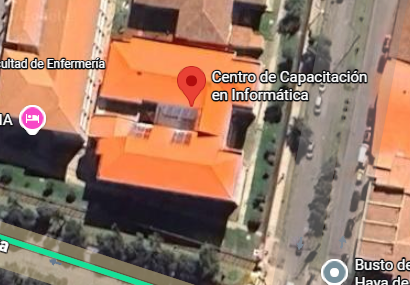
\includegraphics[width=0.7\textwidth]{GoogleMapsInformatica.png}
    \caption{Ubicación de la Facultad de Ingeniería Eléctrica, Electrónica, Informática y Mecánica de la UNSAAC. Av. De la Cultura, Nro. 733, Cusco -- Perú.}
    \label{fig:ubicacion-informatica-unsaac}
\end{figure}

\section{Planos de red, racks y telecomunicaciones}
En esta sección se presentan los planos arquitectónicos base y
las láminas de intervención y mantenimiento correspondientes a
los diferentes niveles del pabellón de Informática de la UNSAAC,
así como la organización de los gabinetes de telecomunicaciones,
patch panels y racks. Los planos detallan la ubicación de los
puntos de red, el trazado de canalizaciones, la distribución de
la infraestructura de telecomunicaciones y la disposición de los
equipos en las salas técnicas y armarios de telecomunicaciones
(MDF e IDF).

% =========================================================
% TERCER PISO
% =========================================================

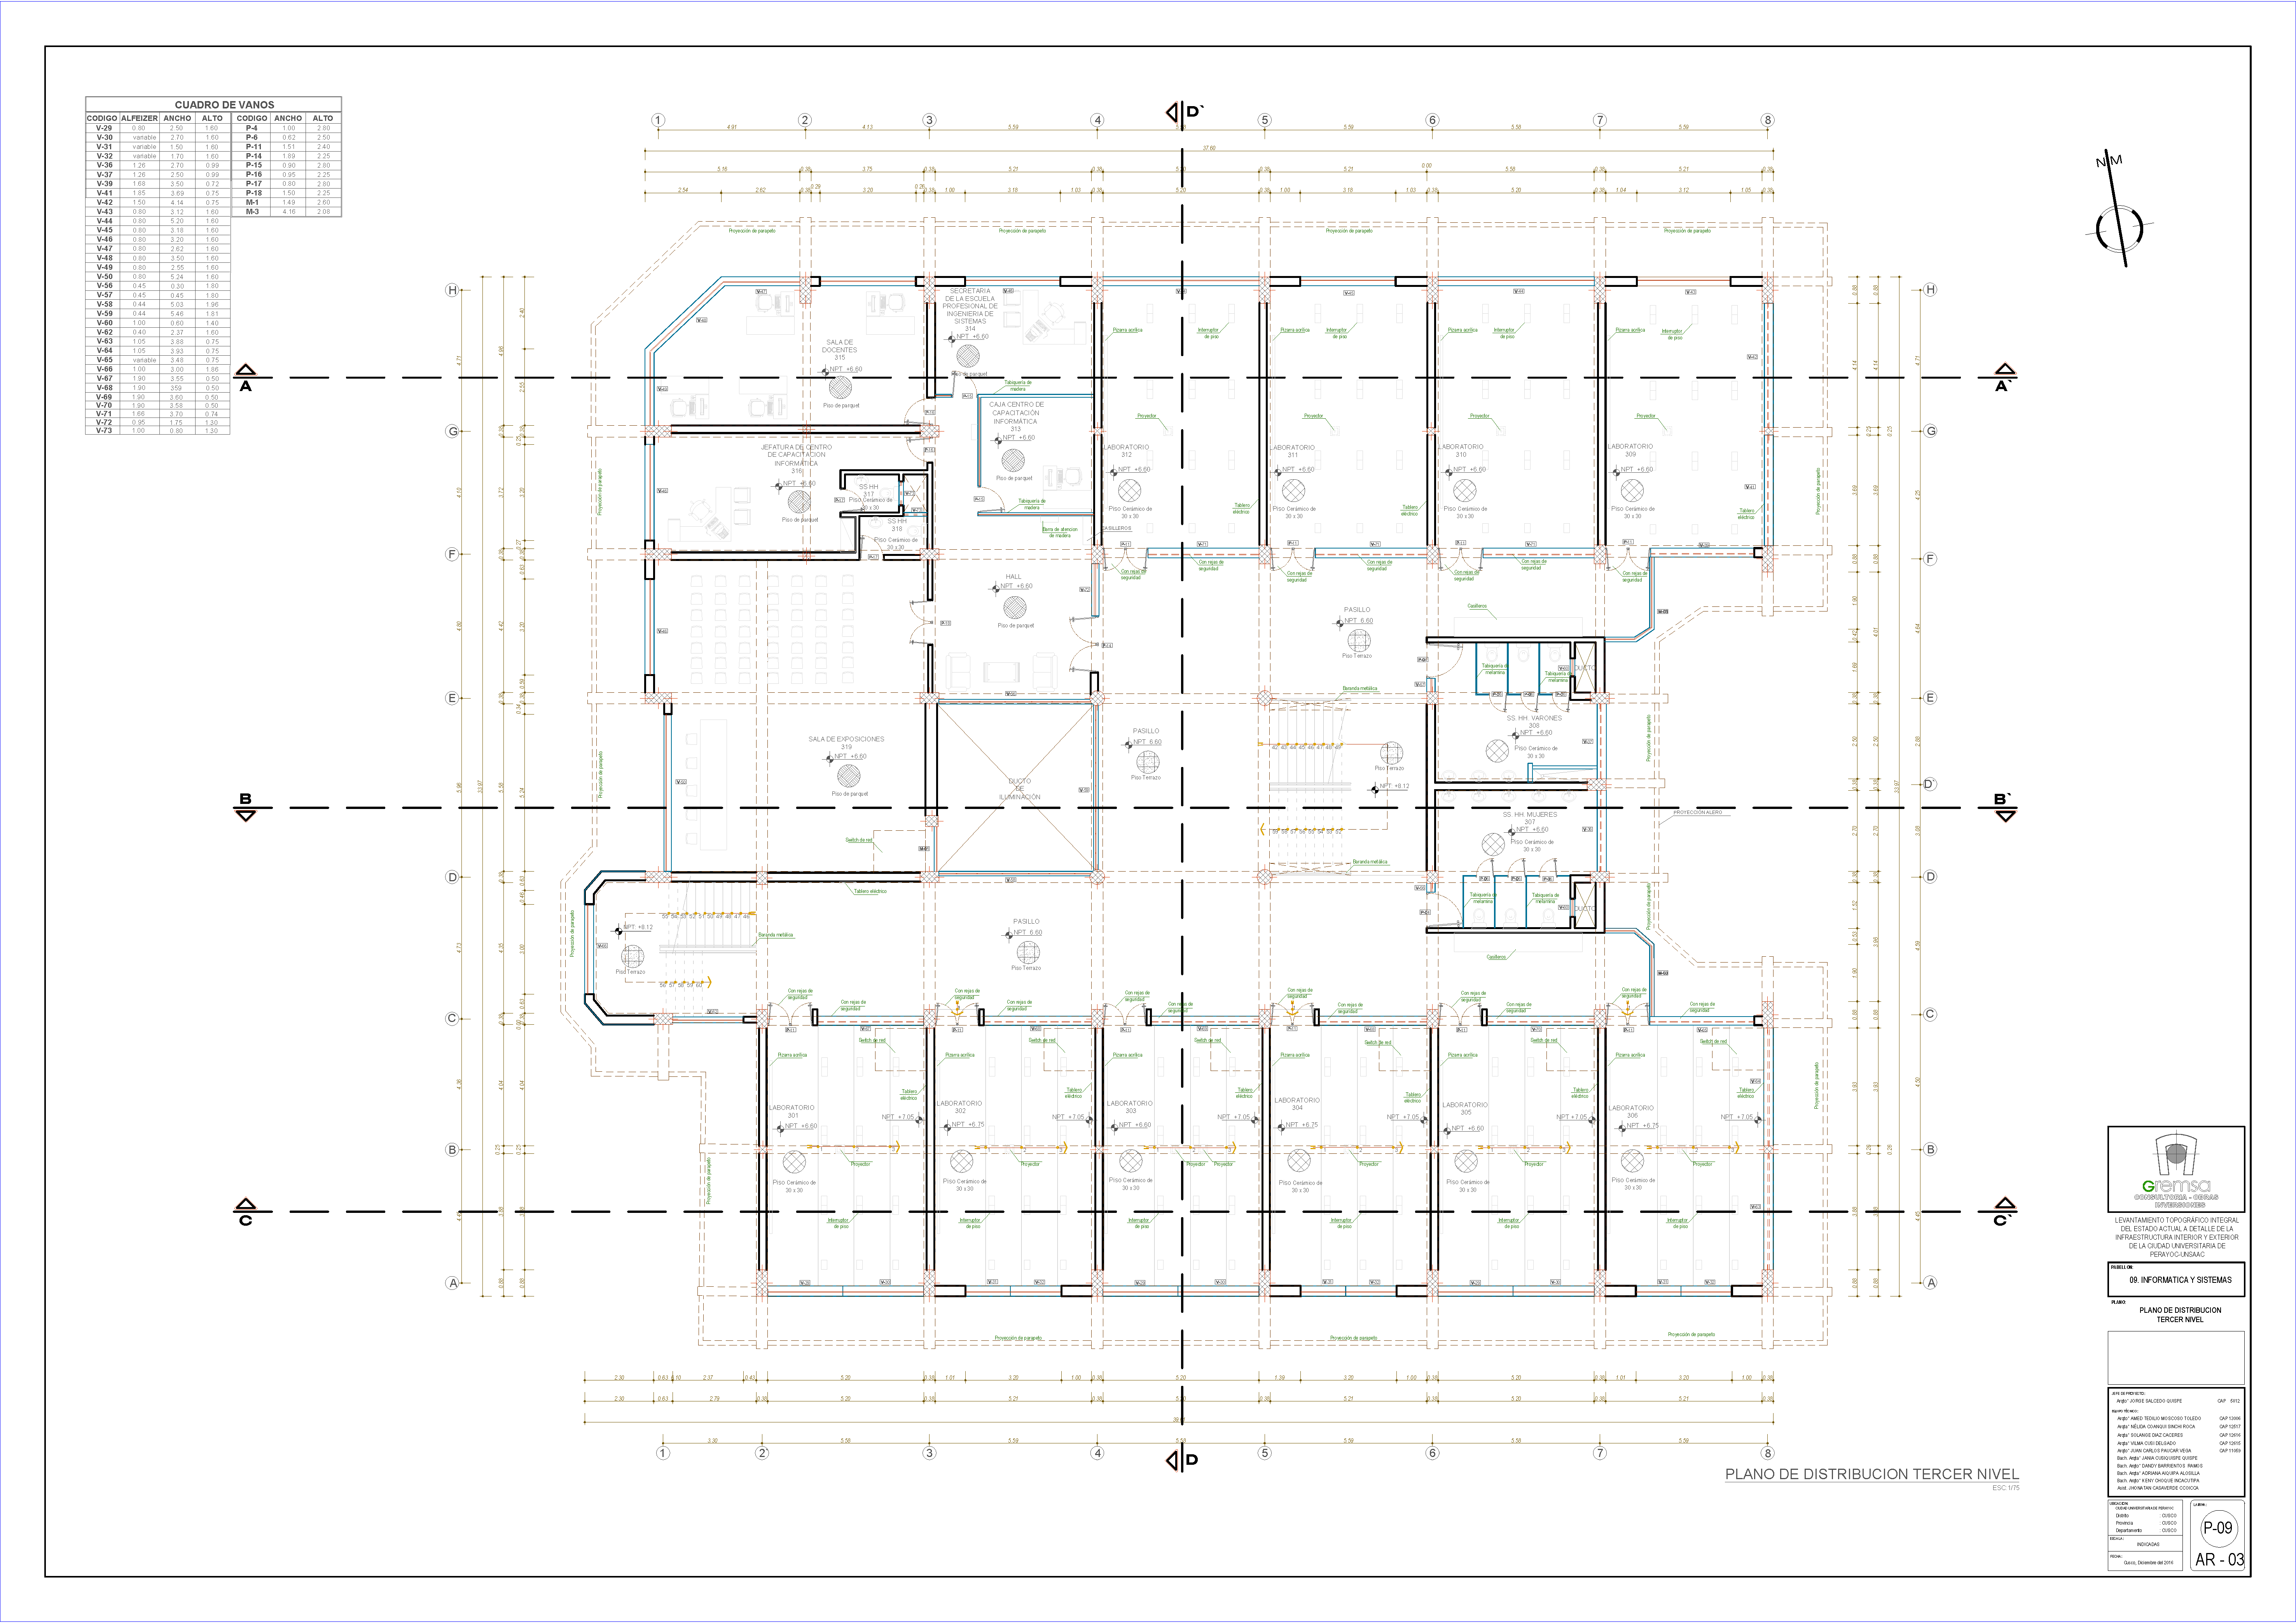
\includepdf[
    pages=1,
    landscape=true,
    scale=0.85,
    pagecommand={
        \section*{Tercer piso -- Plano base (Informatica 3er piso)}
        \thispagestyle{plain}
    }
]{Planos/INFORMATICA_3erPISO.pdf}

% =========================================================
% CUARTO PISO
% =========================================================

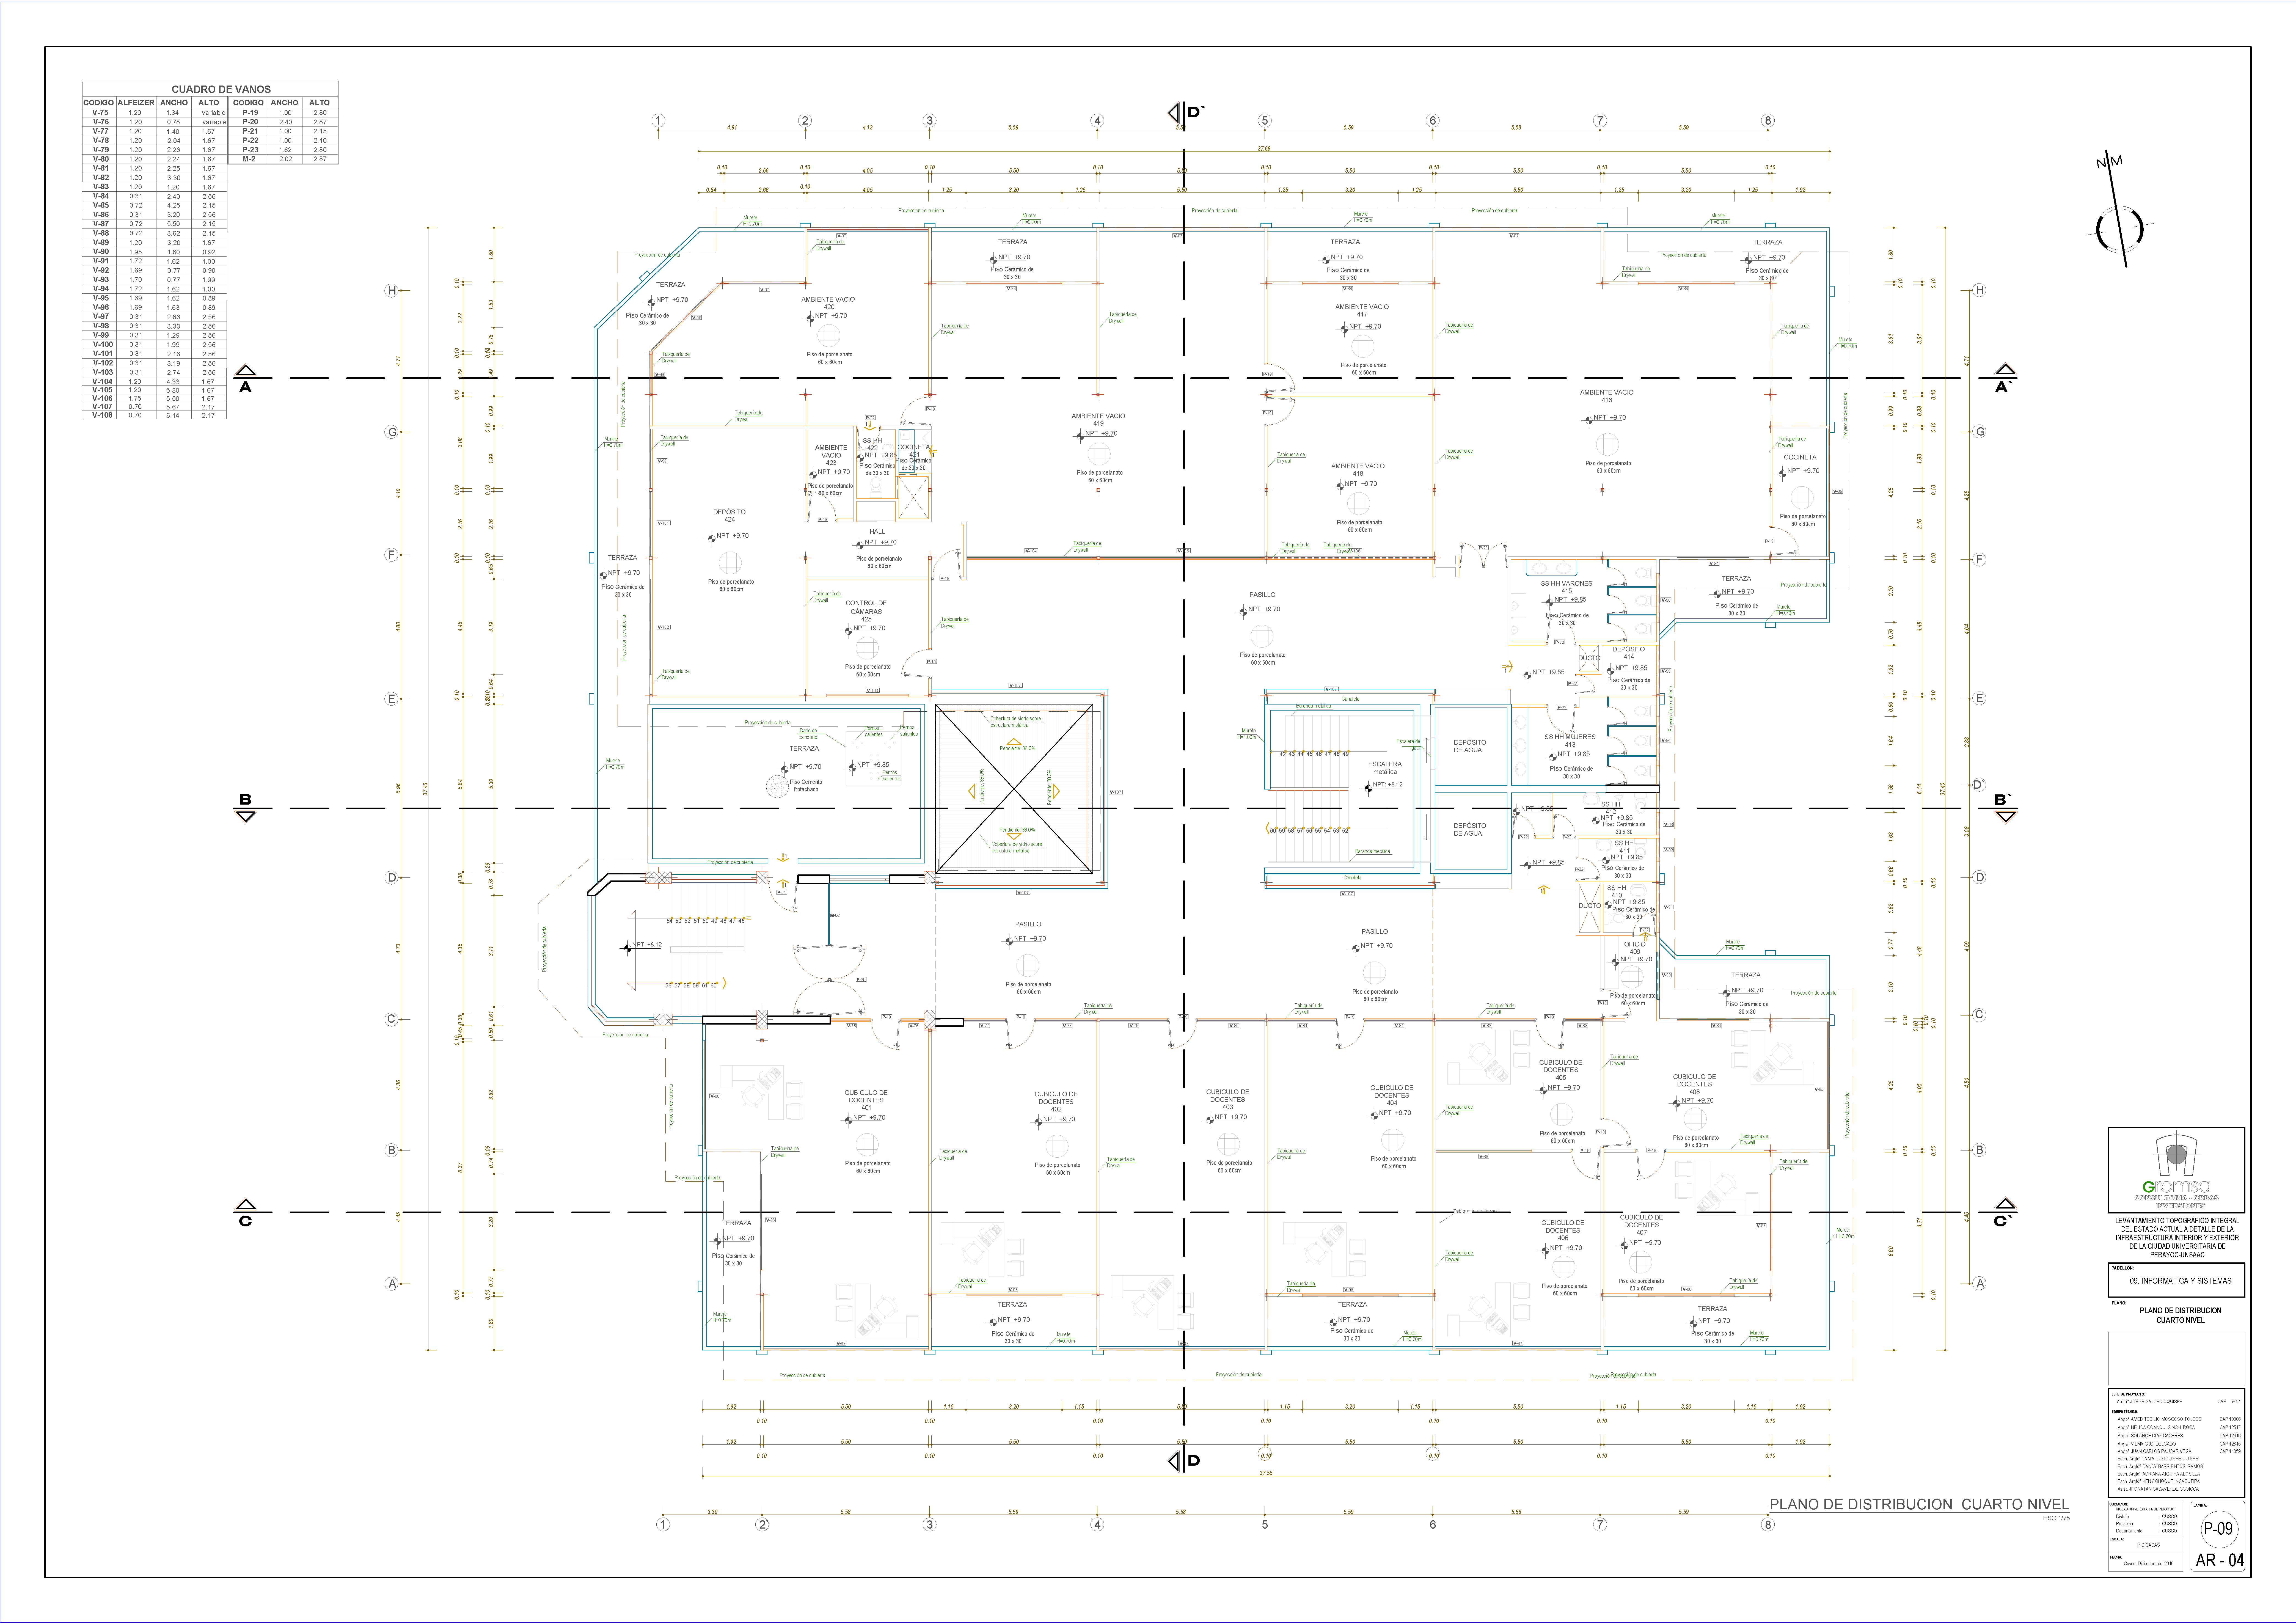
\includepdf[
    pages=1,
    landscape=true,
    scale=0.85,
    pagecommand={
        \section*{Cuarto piso -- Plano base (Informatica 4to piso)}
        \thispagestyle{plain}
    }
]{Planos/INFORMATICA_4toPISO.pdf}

% =========================================================
% TECHO
% =========================================================

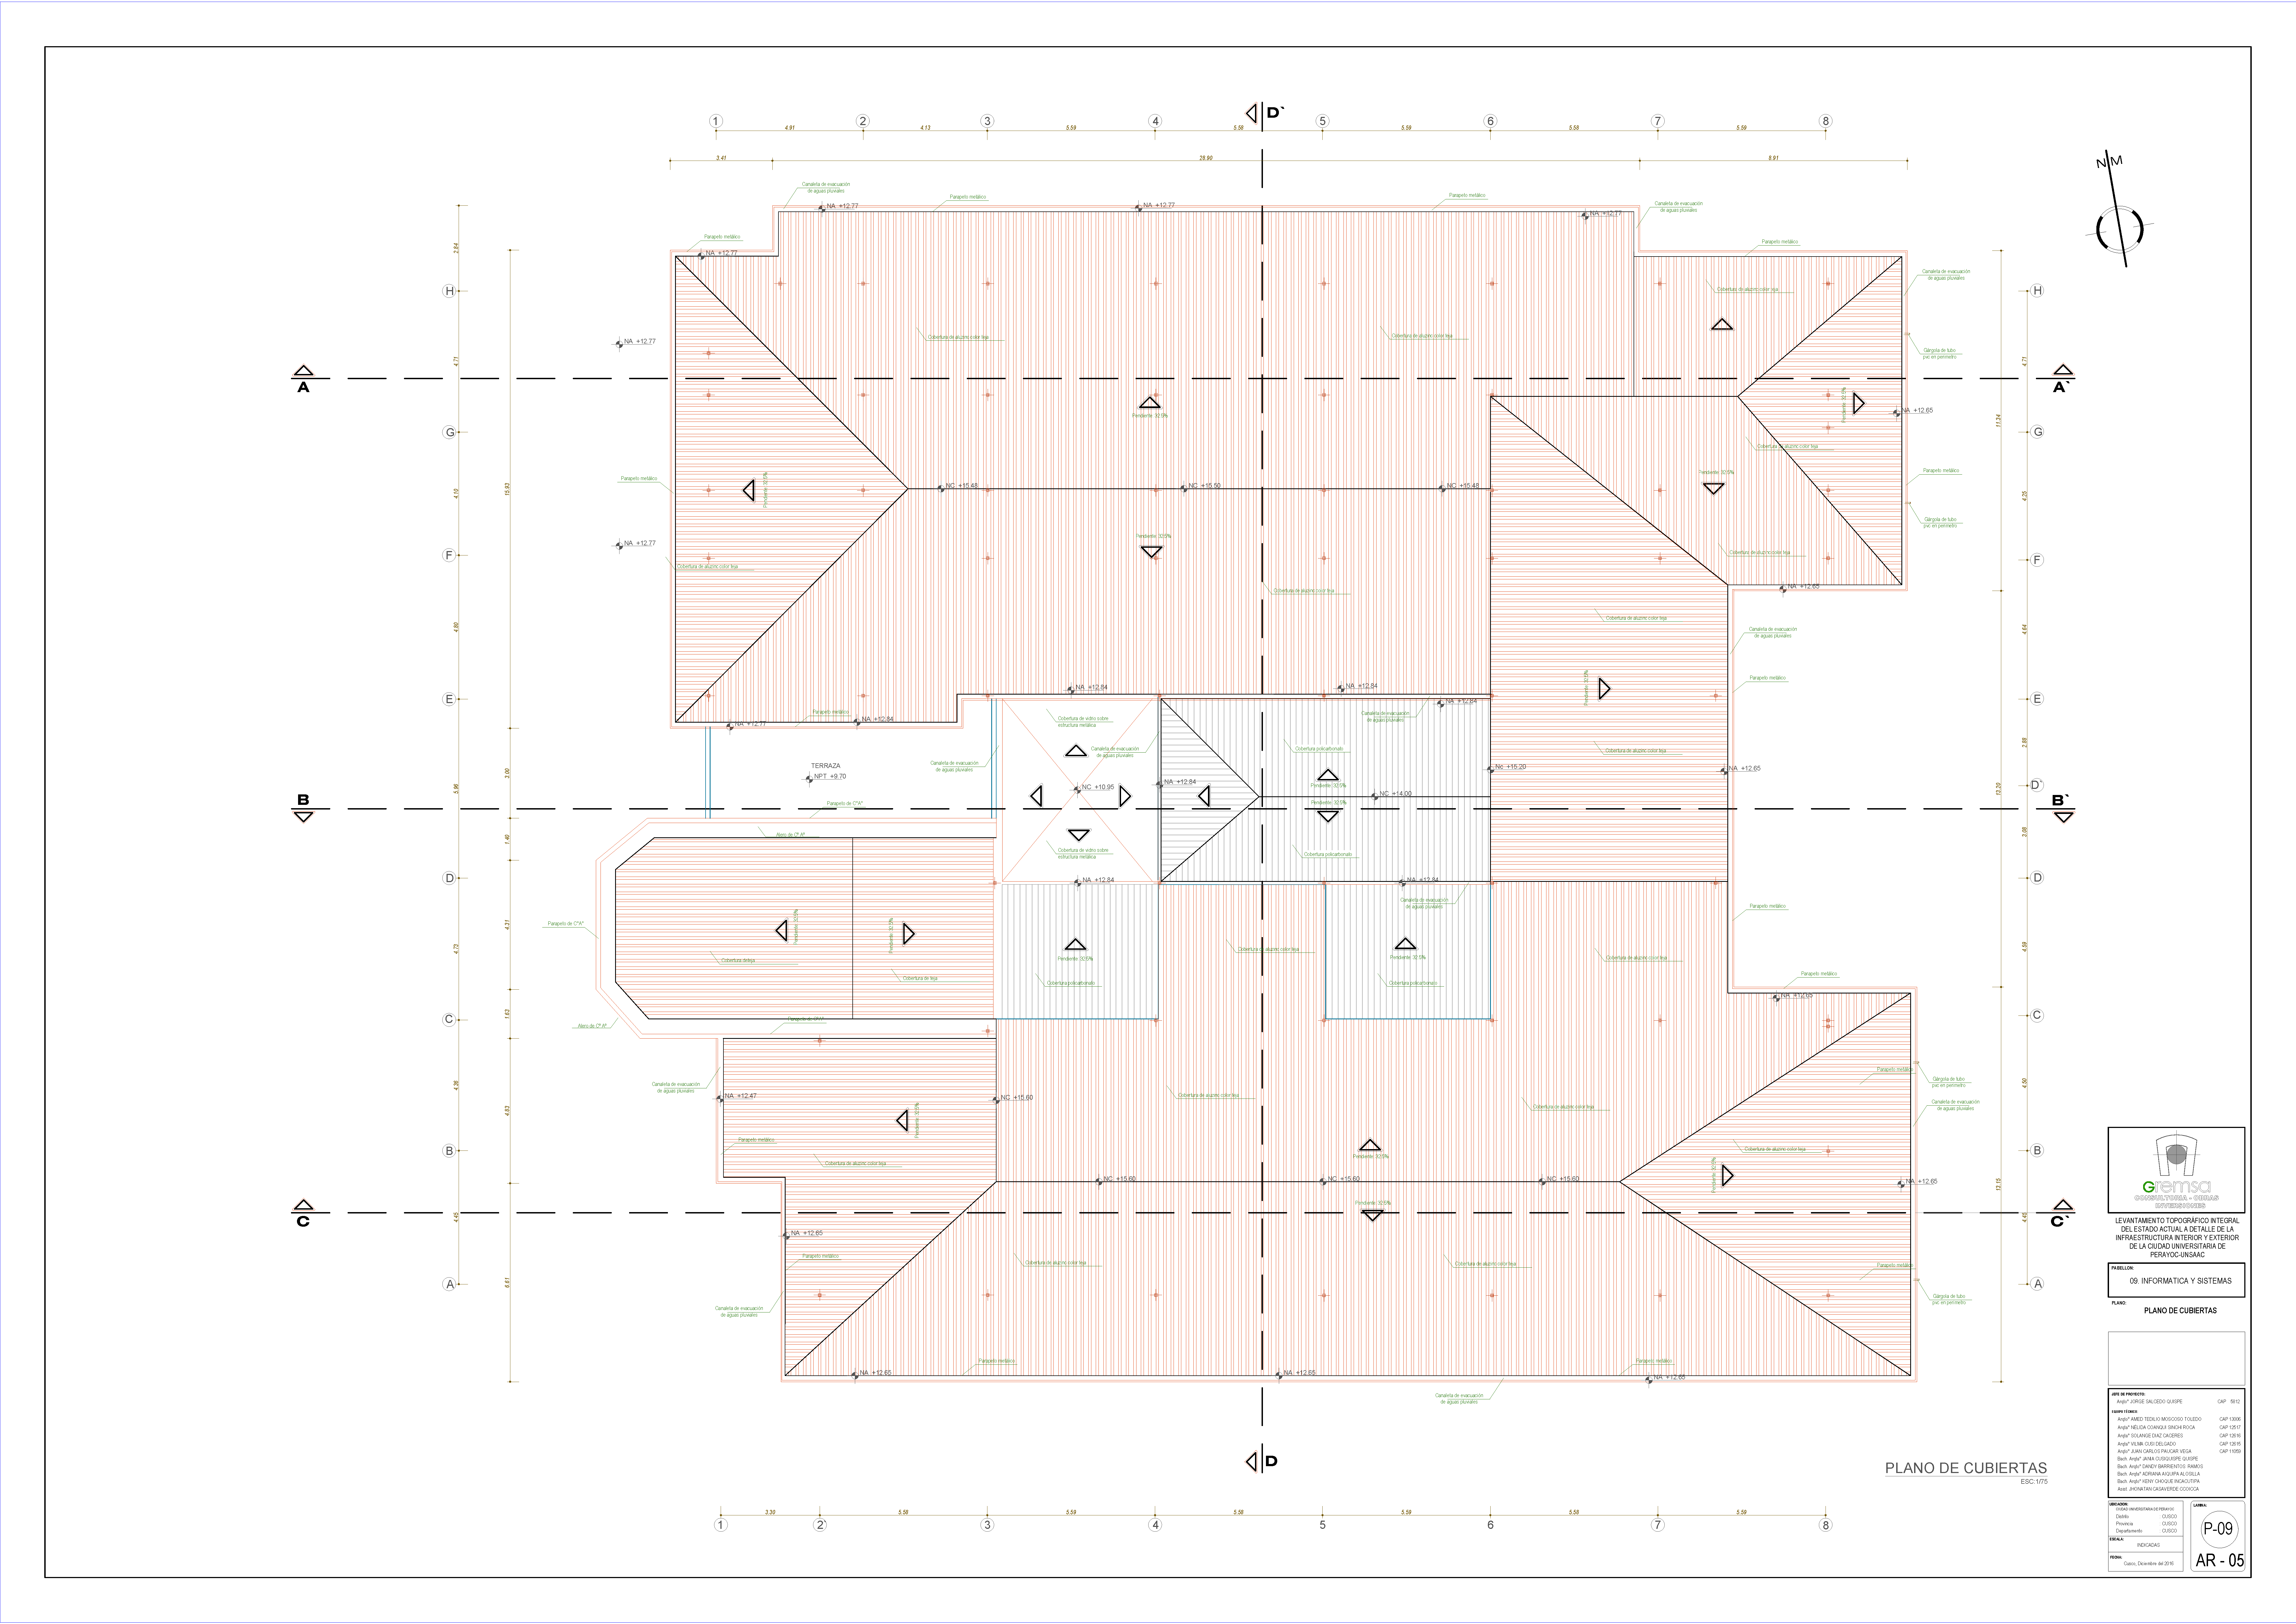
\includepdf[
    pages=1,
    landscape=true,
    scale=0.85,
    pagecommand={
        \section*{Techo -- Plano base (Informatica techo)}
        \thispagestyle{plain}
    }
]{Planos/INFORMATICA_TECHO.pdf}

% =========================================================
% TERCER PISO - Modificado
% =========================================================
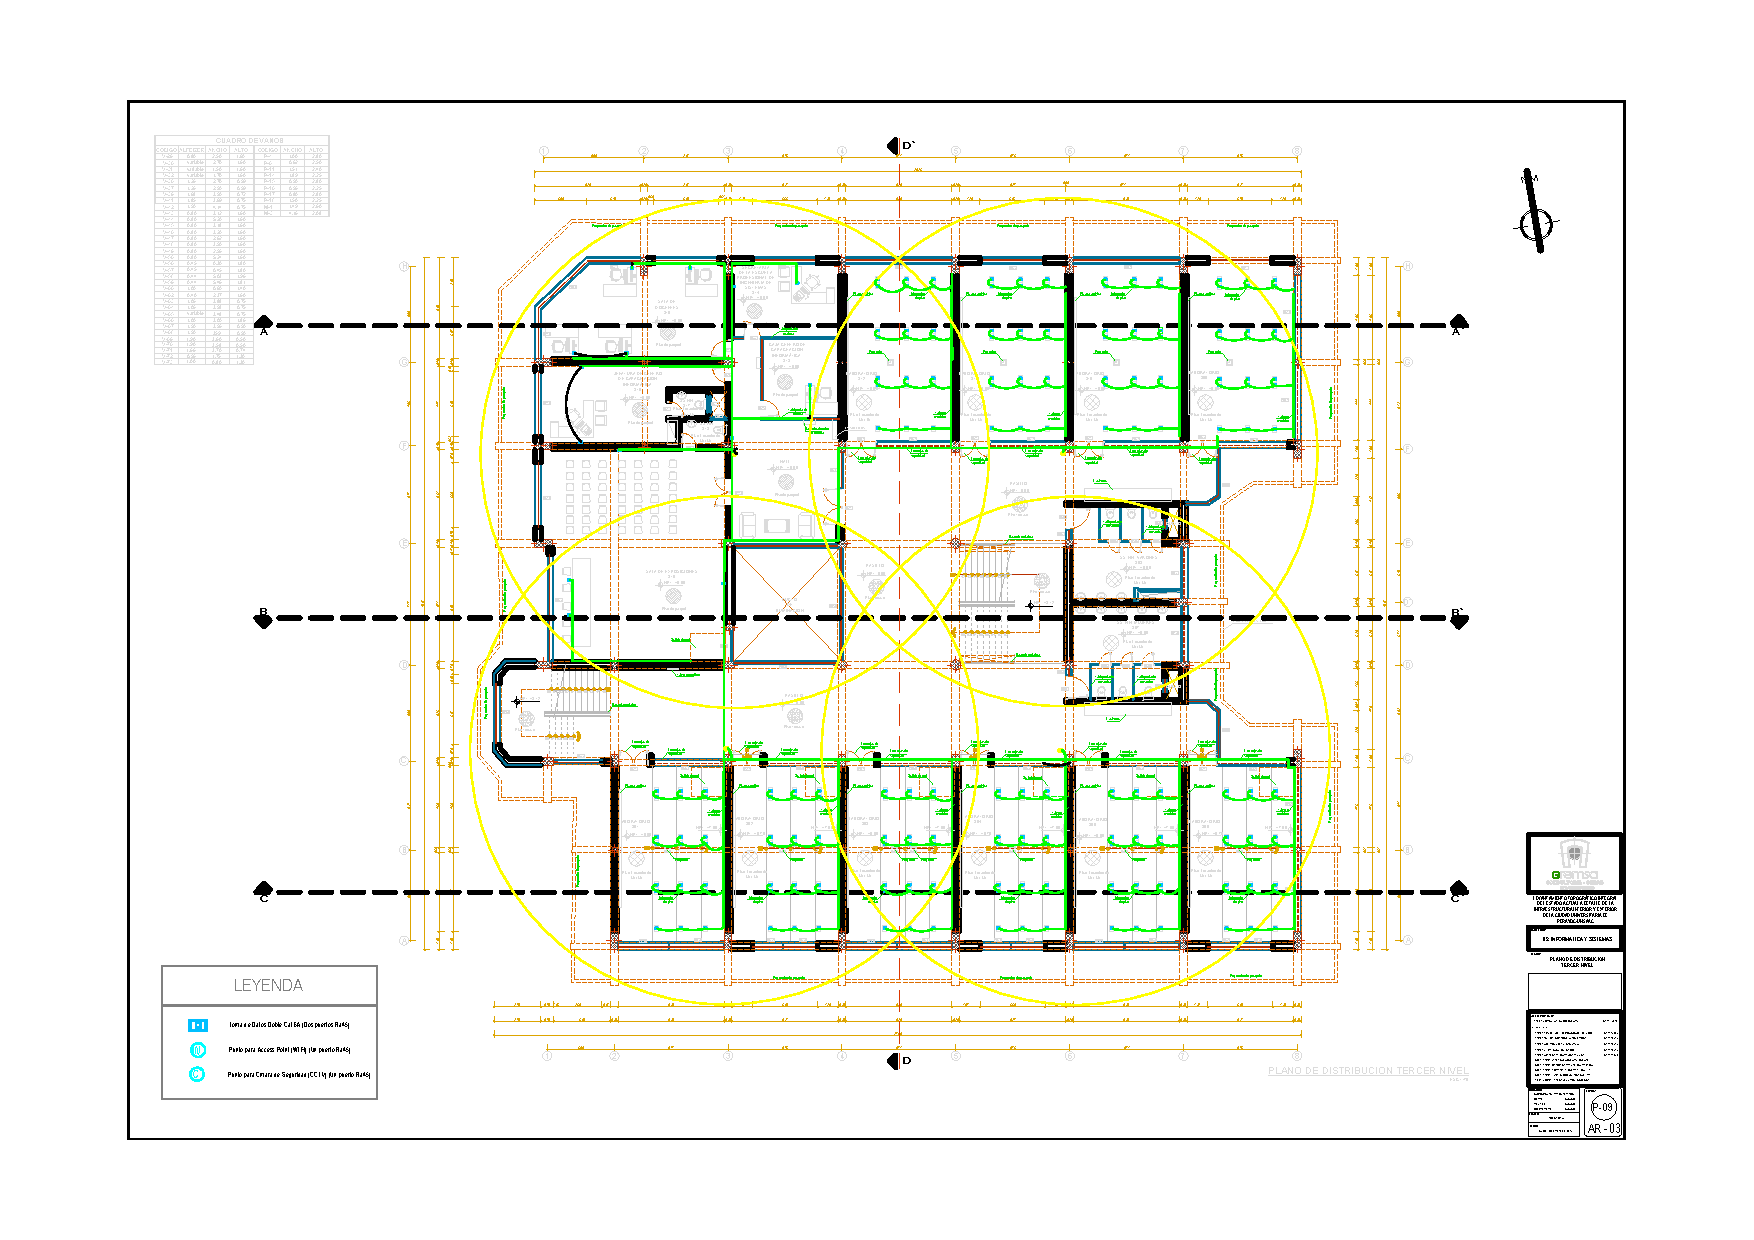
\includepdf[
    pages=1,
    landscape=true,
    scale=0.85,
    pagecommand={
        \section*{Tercer piso -- Plano Modificado (Informatica 3er piso)}
        \thispagestyle{plain}
    }
]{Planos/INFORMATICA_3erPISO_MODIFICADO.pdf}

% =========================================================
% CUARTO PISO - Modificado
% =========================================================
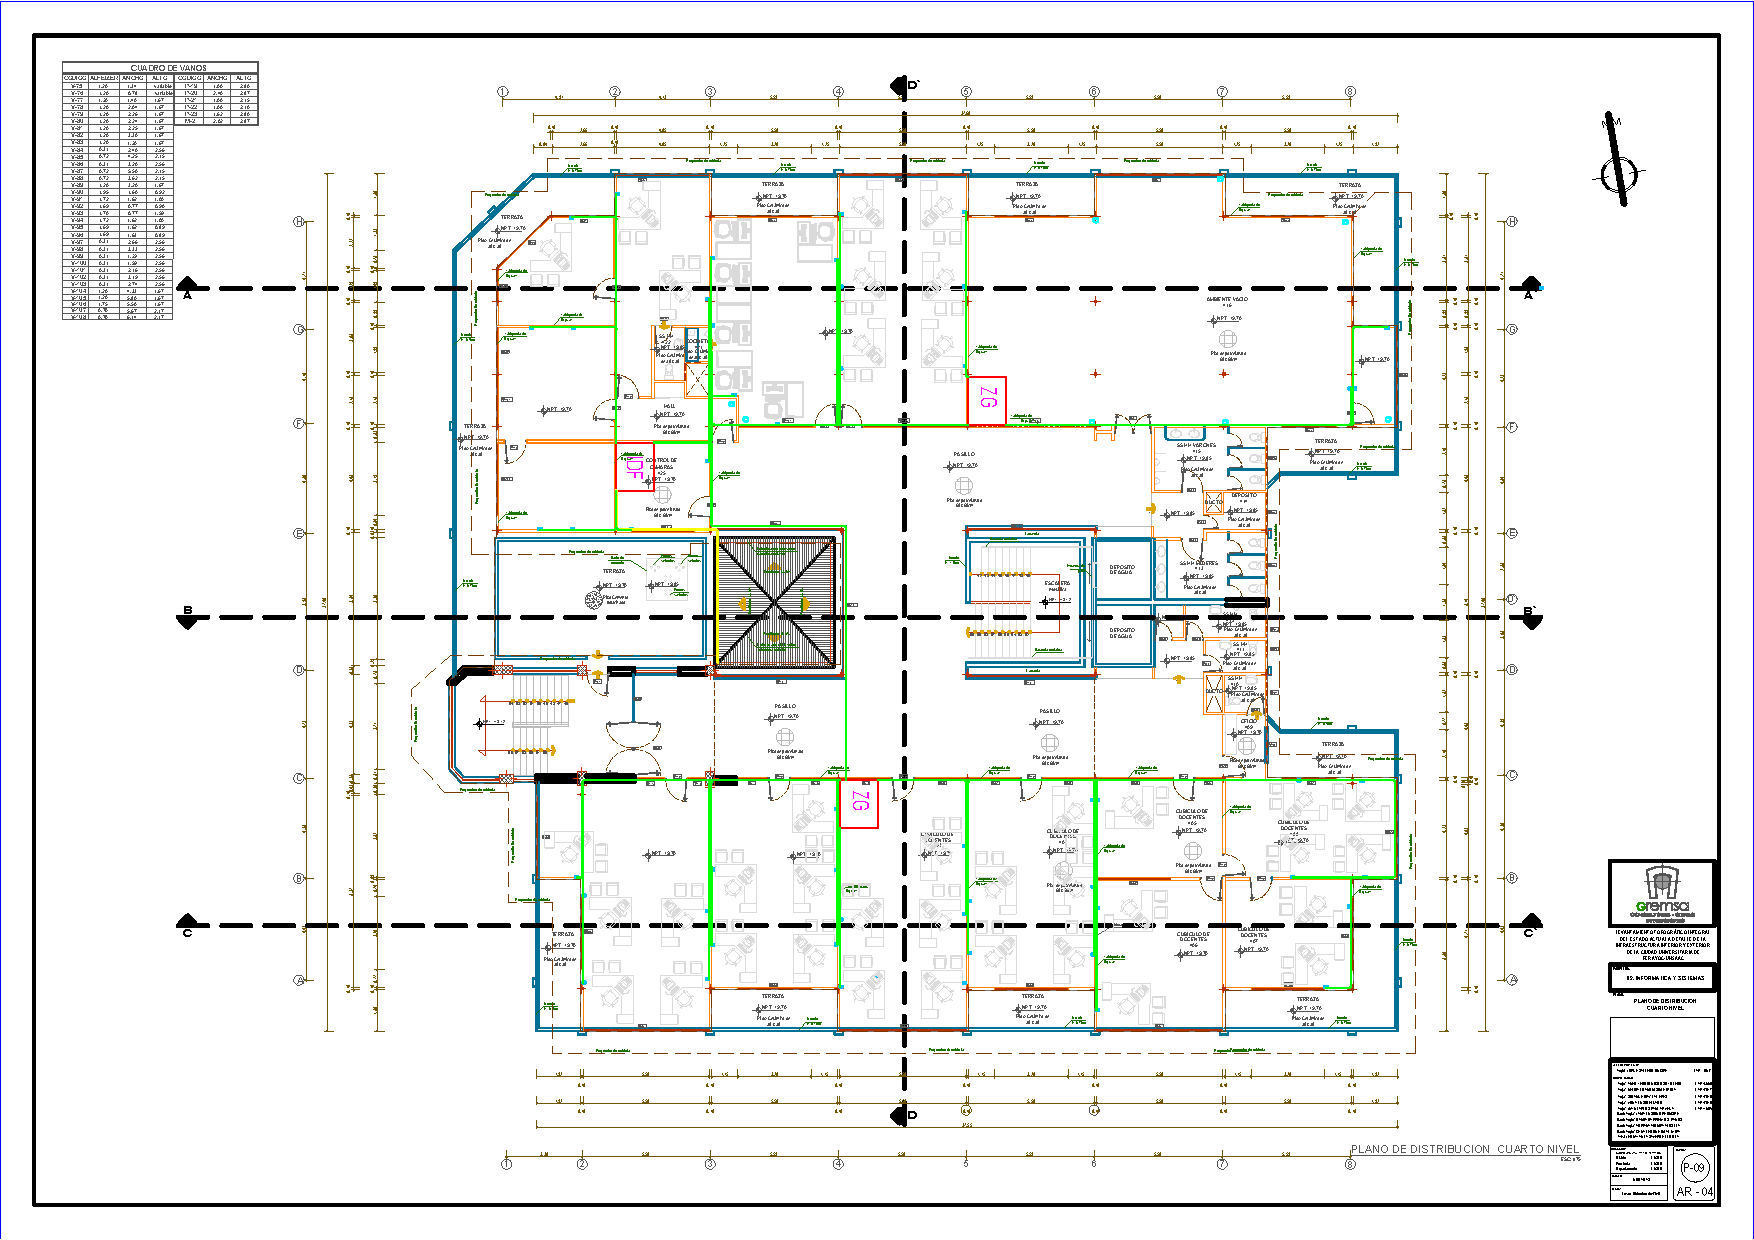
\includepdf[
    pages=1,
    landscape=true,
    scale=0.85,
    pagecommand={
        \section*{Cuarto piso -- Plano Modificado (Informatica 4to piso)}
        \thispagestyle{plain}
    }
]{Planos/INFORMATICA_4toPISO_MODIFICADO.pdf}



\section{Plano de backbone}
Interconexión de armarios principales y secundarios.

\section{Detalles constructivos de ductos, bandejas y registros}
Ductería, bandejas, registros, puesta a tierra.

\section{Diagrama de puesta a tierra}
\chapter{Especificaciones Técnicas}

\section{Tipo y categoría de cables}

Para garantizar el rendimiento requerido en los \totalPisos{} niveles del pabellón de la Escuela Profesional de Ingeniería Informática y de Sistemas de la UNSAAC, se especifica el siguiente esquema de cableado:

\begin{itemize}
    \item \textbf{Cableado Horizontal (Datos, Telefonía IP y CCTV):} Se utilizará cable de par trenzado de cuatro pares del tipo \textbf{F/UTP (Foiled/Unshielded Twisted Pair) Categoría 6A} LSZH (Low Smoke Zero Halogen), marca \textbf{Panduit} modelo \texttt{PUFL6X04WH}. El blindaje general foil protege contra la diafonía exógena (Alien Crosstalk) y las interferencias electromagnéticas (EMI) típicas de los entornos de laboratorios informáticos y equipos eléctricos del edificio. Soporta velocidades de hasta 10 Gbps a frecuencias de 500 MHz, cumpliendo con el estándar IEEE 802.3an (10GBASE-T).
    \item \textbf{Cableado Vertical o Backbone:} Interconexión del Distribuidor Principal de Cableado (MDF) situado en el segundo piso con los Distribuidores de Piso (IDF) del primer, tercer y cuarto piso mediante \textbf{Fibra Óptica Multimodo OM4} de 4 hilos, con chaqueta LSZH, marca \textbf{CommScope} serie \texttt{TeraSPEED}, optimizada para transmisión láser de 10/40/100 Gbps. Se instalarán tres enlaces independientes: MDF (2do piso) a IDF (1er piso), MDF (2do piso) a IDF (3er piso) y MDF (2do piso) a IDF (4to piso), con longitudes estimadas de 20, 20 y 40 metros respectivamente.
    \item \textbf{Cableado para CCTV (Cámaras IP):} Se utilizará cable \textbf{F/UTP Cat 6A} LSZH (mismo tipo que el cableado horizontal) para las cámaras IP de videovigilancia, alimentadas mediante PoE+ desde los switches de acceso. Los puntos de cámara compartirán el mismo esquema de cableado y certificación que los puntos de datos.
    \item \textbf{Patch Cords:} Cables de parcheo F/UTP Cat 6A blindados de 2.1 m y 1.0 m, marca \textbf{Panduit} modelo \texttt{STP6X2MBU} y \texttt{STP6X1MBU}, con conectores blindados RJ-45 moldeados y alivio de tensión integrado. Se suministrarán dos patch cords por cada punto de red instalado (uno para el lado de usuario y otro en el rack).
\end{itemize}

\subsection*{Definición y clasificación de tomas y puertos de red}

Para efectos de control métrico y técnico de este expediente, se establecen las siguientes definiciones de manera unificada:
\begin{itemize}
    \item \textbf{Puerto físico (RJ-45):} Interfaz terminal hembra de 8 hilos blindada que aloja un conector RJ-45.
    \item \textbf{Punto de red (o enlace horizontal):} El canal completo que va desde el jack RJ-45 en el área de trabajo del usuario, discurre por la canalización horizontal y finaliza en el patch panel modular correspondiente en el rack. Cada punto de red equivale exactamente a un puerto activo en el switch.
    \item \textbf{Punto simple:} Toma de red compuesta por un único jack RJ-45 montado en un faceplate de 1 o 2 puertos. Se utiliza para dispositivos dedicados de un solo puerto como APs, cámaras de videovigilancia, proyectores o pizarras digitales.
    \item \textbf{Punto doble:} Toma de red compuesta por dos jacks RJ-45 independientes montados sobre el mismo faceplate de 2 puertos, conectados mediante dos cables F/UTP Cat 6A independientes al patch panel. Se emplea en puestos de trabajo (estaciones de docentes, administrativos y laboratorios) para permitir la conexión paralela de voz (teléfono IP) y datos (PC) sin conmutación local.
    \item \textbf{Punto de reserva:} Enlace de cableado horizontal completo instalado físicamente pero no conectorizado al switch de forma activa, reservado para expansiones o redundancia operativa.
\end{itemize}


\section{Normas de instalación, etiquetado y terminación}

Toda la infraestructura instalada debe ceñirse estrictamente a los estándares internacionales de telecomunicaciones. El aseguramiento de la calidad en la transmisión de datos a 10 Gbps depende no solo de la calidad de los materiales, sino fundamentalmente de la estricta adherencia a los procedimientos técnicos de instalación:

\begin{itemize}
    \item \textbf{Estándares de Diseño e Instalación:} ANSI/TIA-568.0-D (Cableado Genérico para Telecomunicaciones en las Instalaciones del Cliente) y ANSI/TIA-568.1-D (Estándar de Infraestructura de Telecomunicaciones para Edificios Comerciales). Adicionalmente, se cumple con el \textbf{Reglamento Nacional de Edificaciones (RNE)} del Perú, norma EM.010 (Redes e Infraestructura de Telecomunicaciones) y el \textbf{Código Nacional de Electricidad - Utilización (CNE)} para canalizaciones y seguridad eléctrica.
    \item \textbf{Esquema de Terminación:} Se implementará el patrón de conexión \textbf{T568B} de manera uniforme en todos los módulos RJ-45 (jacks), patch panels y patch cords de la obra.
    \item \textbf{Radio de Curvatura Mínimo:} Durante el tendido, se respetará un radio de curvatura mínimo de \textbf{4 veces el diámetro exterior del cable} (aproximadamente 32 mm para cable Cat 6A de 8 mm de diámetro). En ningún caso se excederá este límite, ya que deformaciones en la geometría de los pares trenzados provocan pérdida de retorno y degradación de la señal a 500 MHz.
    \item \textbf{Tensión Máxima de Tracción:} La fuerza de tiro durante el tendido no superará las \textbf{25 libras-fuerza (lbf)} equivalentes a 111 Newtons. Se utilizarán lubricantes apropiados para cableado estructurado en tramos de alta fricción y se evitarán tirones bruscos que puedan estirar el cable y alterar sus propiedades eléctricas.
    \item \textbf{Destrenzado Máximo:} Al momento de la terminación en los conectores (jacks y patch panels), el destrenzado de los pares no excederá los \textbf{13 mm (0.5 pulgadas)} para mantener la inmunidad al ruido (NEXT y FEXT). Valores superiores degradan irreversiblemente el desempeño del enlace.
    \item \textbf{Administración y Etiquetado:} Bajo la norma \textbf{ANSI/TIA-606-C}. Cada punto de red, cable, patch panel y gabinete poseerá una etiqueta impresa térmicamente con un código alfanumérico estructurado siguiendo el formato \textit{Piso - Cuarto de Telecomunicaciones - Rack - Panel - Puerto} (\textit{Ejemplo: 02P-MDF-A1-01} para el Segundo Piso, MDF, Rack A, Panel 1, Puerto 01). Las tomas de usuario contarán con iconos de color para diferenciar redes de datos (azul), telefonía IP (verde) y cámaras de seguridad (rojo).
\end{itemize}

\subsection*{Control de Alien Crosstalk (AXT)}

Dado que el cableado F/UTP Cat 6A opera a frecuencias de hasta 500 MHz, es crítico controlar la diafonía exógena (Alien Crosstalk) entre cables adyacentes, especialmente en los mazos densos que salen de los gabinetes MDF e IDF hacia los laboratorios y aulas:

\begin{itemize}
    \item \textbf{Sujeción:} Se prohíbe terminantemente el uso de cintillos plásticos (zip ties) apretados que deformen la geometría del cable. Se utilizará exclusivamente \textbf{velcro} (cinta enrollable) de forma holgada para agrupar los cables, permitiendo el movimiento natural y evitando puntos de presión que alteren la impedancia del cable.
    \item \textbf{Factor de Llenado:} Se limitará la ocupación de las canaletas al \textbf{40\%} de la sección transversal, conforme a la norma ANSI/TIA-569-D. Esto permite que los cables se acomoden aleatoriamente (random lay), reduciendo naturalmente la alineación de pares y cancelando el ruido entre cables vecinos.
    \item \textbf{Separación de Servicios:} Se mantendrá una separación física mínima de \textbf{200 mm (8 pulgadas)} entre el cableado de datos F/UTP Cat 6A y cualquier línea eléctrica de potencia (220V) que corra en paralelo. En áreas de espacio reducido donde esta separación no sea viable, se instalarán barreras físicas metálicas conectadas a tierra.
    \item \textbf{Cruces Perpendiculares:} Cualquier intersección necesaria entre la ruta de datos y los circuitos eléctricos se ejecutará obligatoriamente en un ángulo de \textbf{90 grados} para anular la inducción magnética.
\end{itemize}

\section{Estándares de racks, gabinetes y salas de telecomunicaciones}

La infraestructura de soporte físico se regirá bajo el estándar EIA/ECA-310-E (dimensiones de 19 pulgadas) y ANSI/TIA-569-D (espacios de telecomunicaciones). Se priorizará el uso de gabinetes cerrados (enclosures) sobre racks abiertos para garantizar la seguridad física, la protección contra polvo y humedad, y el control de acceso:

\begin{itemize}
    \item \textbf{Distribuidor de Piso (IDF - 1er Piso):} Gabinete de piso/pared de \textbf{24U}, ubicado en el cuarto de telecomunicaciones acondicionado bajo la escalera principal del primer piso. Permite alimentar las aulas y oficinas administrativas de dicho nivel sin exceder los límites de longitud horizontal del cableado.
    \item \textbf{Distribuidor Principal (MDF - 2do Piso):} Gabinete de piso autocualificado de \textbf{19 pulgadas} de ancho útil y una altura de \textbf{42U}. Profundidad mínima de 1000 mm para alojar equipos de gran profundidad y gestionar holgadamente el cableado Cat 6A. Cumplirá con el estándar EIA-310-E, con puertas microperforadas (frontal y trasera) para optimizar el flujo de aire, cerradura de seguridad con llave y paneles laterales desmontables. Alojará los servidores locales, switches troncales, patch panels del segundo piso y el panel de fibra óptica principal.
    \item \textbf{Distribuidor de Piso (IDF - 3er Piso):} Gabinete de piso/pared de \textbf{24U}, ubicado estratégicamente en un cuarto de telecomunicaciones dedicado en el tercer piso para no superar el límite de 90 metros de canalización horizontal hacia los laboratorios de cómputo.
    \item \textbf{Distribuidor de Piso (IDF - 4to Piso):} Gabinete de piso/pared de \textbf{24U}, ubicado para alimentar los cubículos de docentes, auditorio, laboratorio de investigación y control de cámaras del cuarto piso.
    \item \textbf{Ordenadores de Cable:} Se instalarán organizadores horizontales de 1U con ducto ranurado frontal y tapa desmontable entre cada patch panel, y organizadores verticales dentro de los gabinetes para asegurar un radio de curvatura correcto en los cables de parcheo y mantener el orden.
    \item \textbf{Anclaje Antisísmico:} Considerando la ubicación del proyecto en Cusco (zona sísmica), todos los gabinetes se fijarán al piso mediante pernos de expansión tipo Hilti de 3/8" o 1/2". En el caso de gabinetes adosados a pared, se verificará que el muro sea de concreto o ladrillo macizo para soportar el torque de carga. En el cuarto piso, al ser muros de drywall, se aplicará un refuerzo estructural con planchas de madera contrachapada y anclaje superior de seguridad a la losa de techo.
\end{itemize}

\subsection*{Criterios de diseño de salas de telecomunicaciones}

Cada cuarto de telecomunicaciones (MDF e IDF) deberá cumplir con los siguientes requisitos mínimos:

\begin{itemize}
    \item \textbf{Áreas de Trabajo (Clearance):} Espacio libre mínimo de \textbf{1.0 metro} tanto en la parte frontal como posterior del gabinete para permitir la apertura total de puertas, el ingreso de aire frío para ventilación y la maniobra técnica segura durante la certificación y el parcheo.
    \item \textbf{Ventilación y Climatización:} Los recintos designados requieren ventilación asistida (extractores o aire acondicionado) para disipar el calor generado por los equipos activos (switches PoE+ que pueden disipar hasta 300W cada uno) y las baterías de los UPS, evitando la degradación de la vida útil de los componentes electrónicos.
    \item \textbf{Iluminación:} Nivel de iluminación mínimo de 500 lux en el plano vertical frontal de los gabinetes para facilitar las labores de parcheo, mantenimiento y certificación.
    \item \textbf{Capacidad Portante del Piso:} Se estima que un gabinete completamente equipado (switches + UPS + baterías + cableado) puede alcanzar un peso dinámico de 150 a 250 kg. Las losas de concreto deben ser aptas para soportar esta carga puntual.
    \item \textbf{Tomas Eléctricas Dedicadas:} Cada cuarto de telecomunicaciones contará con circuitos eléctricos independientes de 20A o 30A con tierra aislada, dedicados exclusivamente a los equipos de red, minimizando el riesgo de sobrecargas por conexión de equipos no autorizados.
\end{itemize}

\subsection*{Equipos Pasivos}

\begin{itemize}
    \item \textbf{Patch Panels:} Módulos modulares descargados de 24 puertos Cat 6A angulares, marca \textbf{CommScope} modelo \texttt{760237040}, para optimizar el espacio y evitar el estrés mecánico en los patch cords. Se instalarán un total de 15 paneles distribuidos para atender de forma ordenada la densidad de puntos: 2 paneles en el IDF del 1er piso, 3 en el MDF (2do piso), 6 en el IDF del 3er piso y 4 en el IDF del 4to piso (dando un total de 360 puertos disponibles para los \totalPuntos{} puntos activos).
    \item \textbf{Jacks y Conectores:} Módulos RJ-45 Mini-Com Cat 6A blindados, marca \textbf{Panduit} modelo \texttt{CJS6X88TGY}, con tecnología de terminación por desplazamiento de aislante (IDC) y contacto de 50 micras de oro.
    \item \textbf{Faceplates y Cajas de Montaje:} Placas faceplate de 2 puertos color blanco, marca \textbf{Panduit} modelo \texttt{CFPL2EIWH}, con etiquetado iconográfico integrado para datos (azul), voz (verde) y CCTV (rojo). Se instalarán sobre cajas superficiales de PVC de 1 módulo en paredes y canaletas.
    \item \textbf{Patch Cords:} Cables de parcheo F/UTP Cat 6A blindados, marca \textbf{Panduit} modelo \texttt{STP6X2MBU} (2.1 m) y \texttt{STP6X1MBU} (1.0 m), con conectores blindados RJ-45 moldeados y alivio de tensión. Se suministrarán dos unidades por cada punto de red (uno para el lado del usuario y otro para el lado del patch panel) totalizando \totalPuntos{} unidades de cada longitud.
    \item \textbf{Organizadores de Cable:} Organizadores horizontales de 1U con ducto ranurado frontal y tapa desmontable, marca \textbf{Tripp Lite} modelo \texttt{NR2600}, instalados entre cada patch panel. Organizadores verticales dentro de cada gabinete para el guiado de cables de parcheo.
    \item \textbf{Canalizaciones:} Escalerillas portacables de tipo malla electrozincada en pasadizos principales (\metrosEscalerilla{} metros estimados), canaletas de PVC de doble vía con división física para datos y energía en oficinas y laboratorios (\metrosCanaleta{} metros), y tubería corrugada de 1 pulgada para la protección del backbone de fibra óptica entre pisos (\metrosTuboConduit{} metros).
    \item \textbf{Sistema de Puesta a Tierra:} Barra de Puesta a Tierra Principal de Telecomunicaciones (TMGB) en el MDF del segundo piso, marca \textbf{Panduit} modelo \texttt{TMGB-060}, conectada directamente al pozo a tierra general del edificio mediante conductor de cobre desnudo calibre \textbf{2 AWG} (35 mm$^2$) en el menor recorrido posible y sin empalmes. Barras secundarias (TGB) marca \textbf{Panduit} modelo \texttt{TGB-040} en los IDF del primer, tercer y cuarto piso, interconectadas a la TMGB mediante conductores de cobre aislado verde 6 AWG.
\end{itemize}

\subsection*{Equipos Activos}

\begin{itemize}
    \item \textbf{Switches de Acceso:} Switches gestionables de Capa 2/3 con soporte \textbf{PoE+ (Power over Ethernet - IEEE 802.3at)} marca \textbf{Cisco} serie \textbf{Catalyst 9200}, modelos \texttt{C9200-48P-E} (\totalSwitchesCuarentaYOcho{} unidades) y \texttt{C9200-24P-E} (\totalSwitchesVeinticuatro{} unidad), con puertos de bajada a 1 Gbps Base-T y uplinks de 10 Gbps SFP+ para el backbone de fibra óptica. Se distribuirán: 1x C9200-48P-E en el IDF del 1er piso, 1x C9200-48P-E y 1x C9200-24P-E en el MDF (2do piso), 3x C9200-48P-E en el IDF del 3er piso y 2x C9200-48P-E en el IDF del 4to piso.
    \item \textbf{Transceptores SFP+:} Módulos SFP+ multimodo 10 GBase-SR, marca \textbf{Cisco} modelo \texttt{SFP-10G-SR}, para los enlaces de fibra entre el MDF del segundo piso y los IDF del primer, tercer y cuarto piso (6 unidades en total: 2 transceptores por enlace).
    \item \textbf{Puntos de Acceso Inalámbrico (WiFi 6):} Access Points de interior doble banda (2.4 GHz / 5 GHz) con soporte \textbf{WiFi 6 (802.11ax)}, marca \textbf{Cisco} modelo \texttt{C9120AXI}, alimentados mediante PoE+. Se instalarán estratégicamente en pasadizos y ambientes comunes de los cuatro niveles (\totalAP{} unidades en total, distribuidos a razón de 4 APs por piso) para brindar cobertura inalámbrica en laboratorios, auditorio, sala de reuniones, círculos de estudio, biblioteca y áreas administrativas.
    \item \textbf{Cámaras IP (CCTV):} Cámaras IP fijas de interior con resolución mínima de 2 MP (1920x1080), PoE+, marca \textbf{Dahua} o \textbf{Hikvision}, conectadas a los switches de acceso PoE+. Se proyecta un total de \totalCamaras{} cámaras (3 unidades por nivel) integradas con el NVR (Network Video Recorder) de 16 canales que se ubicará en el gabinete MDF del segundo piso para la grabación y gestión centralizada de video.
    \item \textbf{UPS:} Sistemas de alimentación ininterrumpida en línea de doble conversión, marca \textbf{Tripp Lite} modelo \texttt{SU3000RTX} (3kVA), un equipo por cada gabinete (IDF 1er piso + MDF 2do piso + IDF 3er piso + IDF 4to piso = \totalUPS{} unidades en total), con autonomía mínima de 15 minutos a plena carga para salvaguardar la operatividad de los switches, APs y cámaras.
    \item \textbf{PDU:} Unidades de Distribución de Energía rackeables, marca \textbf{Tripp Lite} modelo \texttt{PDU1230}, con entrada monofásica y múltiples salidas NEMA 5-15R/5-20R, una por cada gabinete (\totalPDU{} unidades en total).
\end{itemize}

\section{Canalizaciones, registros y detalles constructivos}

El sistema de canalizaciones constituye la infraestructura de soporte físico que alberga y protege el cableado estructurado. Se divide en canalización principal, canalización secundaria y sistema de registros:

\subsection*{Canalización Principal (Escalerillas Tipo Malla)}

\begin{itemize}
    \item \textbf{Tipo:} Escalerilla portacables de malla electrozincada (tipo rejilla), fabricada en acero al carbono con recubrimiento electrozincado, cumpliendo con la norma ANSI/TIA-569-D y NEMA VE 1.
    \item \textbf{Dimensiones:} Ancho mínimo de 300 mm y profundidad de 50 mm, con separación entre alambres de 50 mm x 100 mm.
    \item \textbf{Soportería:} Instalada cada 1.5 metros sobre soportes tipo L o mensualas metálicas fijadas a losas o paredes mediante pernos de expansión. En tramos horizontales en pasillos principales, se fijará al techo o bajo el falso techo.
    \item \textbf{Rutas:} Discurrirá por los pasillos principales de distribución de cada nivel (primer, segundo, tercero y cuarto piso), conectando los gabinetes MDF/IDF con las zonas de distribución secundaria.
    \item \textbf{Tapas:} En tramos donde la escalerilla cruce zonas accesibles al público, se instalará tapa metálica desmontable para protección mecánica del cableado.
\end{itemize}

\subsection*{Canalización Secundaria (Canaletas PVC y Tuberías)}

\begin{itemize}
    \item \textbf{Canaletas PVC:} Canaletas de PVC rígido autoextinguible (libre de halógenos), de doble compartimiento con divisor físico central para segregación datos/energía. Dimensiones mínimas de 40 mm x 20 mm (2 vías). Se instalarán adosadas a pared en oficinas, laboratorios y cubículos, desde la escalerilla principal hasta cada punto de red.
    \item \textbf{Tubería Conduit:} Para el backbone de fibra óptica entre pisos se utilizará tubería conduit metálica (EMT) de 1 pulgada de diámetro, con accesorios de unión y curvas de radio largo que garanticen el radio de curvatura mínimo de la fibra OM4 (10 veces el diámetro exterior).
    \item \textbf{Factor de Llenado:} En ningún caso la ocupación de cables superará el \textbf{40\%} del área transversal de la canaleta o tubería, conforme a la norma ANSI/TIA-569-D.
    \item \textbf{Separación de Servicios:} Se mantendrá una separación mínima de 200 mm entre canalizaciones de datos y circuitos eléctricos de 220V. En espacios reducidos se usarán canaletas con divisor metálico conectado a tierra.
\end{itemize}

\subsection*{Registros de Paso y Cajas de Derivación}

\begin{itemize}
    \item \textbf{Registros de Paso:} Se instalarán cajas de registro metálicas o de PVC cada 15 metros lineales de canalización, en cada cambio de dirección superior a 30 grados y en los puntos de derivación hacia ambientes específicos. Dimensiones mínimas de 100 mm x 100 mm x 50 mm.
    \item \textbf{Cajas de Paso en Pisos:} Para los tendidos verticales entre niveles (montantes), se instalarán buzones de paso metálicos en cada losa, con dimensiones mínimas de 200 mm x 200 mm, provistos de sellos cortafuego intumescentes para mantener la integridad de la losa contra incendios.
    \item \textbf{Sellado Cortafuego:} Todo pase de cableado entre pisos o a través de muros cortafuego deberá ser sellado con masilla intumescente certificada, manteniendo la clasificación de resistencia al fuego de la estructura (mínimo 2 horas RF-120).
\end{itemize}

\subsection*{Detalles Constructivos}

\begin{itemize}
    \item \textbf{Soportería de Bandejas:} Las escalerillas se soportarán sobre estructuras metálicas tipo L cada 1.5 m, fijadas a losa o pared con pernos de expansión de 3/8". En tramos paralelos a tuberías eléctricas, se interpondrá una barrera metálica conectada a tierra.
    \item \textbf{Curvas y Derivaciones:} Se utilizarán curvas prefabricadas de radio largo (mínimo 300 mm) para garantizar el radio de curvatura del cable Cat 6A. No se aceptarán curvas realizadas en obra mediante doblado de canaletas.
    \item \textbf{Fijación de Canaletas:} Las canaletas PVC se fijarán a la pared cada 40 cm mediante tacos y tornillos de expansión, con tapas de registro cada 2 metros para facilitar el mantenimiento.
    \item \textbf{Amarre de Cables:} Los cables se fijarán a las escalerillas mediante velcro cada 1 metro, sin apretar para no deformar la geometría del par trenzado. Se prohíbe el uso de cintillos plásticos.
\end{itemize}

\section{Requisitos eléctricos y de puesta a tierra}

\subsection*{Sistema de Puesta a Tierra para Telecomunicaciones}

En cumplimiento estricto con las normas \textbf{ANSI/TIA-607-D} y \textbf{ANSI/TIA-607-C}, se implementará un sistema de puesta a tierra dedicado para telecomunicaciones que garantice la protección de los equipos activos y la estabilidad de la transmisión de datos:

\begin{itemize}
    \item \textbf{Barra Principal (TMGB):} Ubicada en el MDF del segundo piso, marca \textbf{Panduit} modelo \texttt{TMGB-060}, conectada directamente al pozo a tierra general del edificio mediante conductor de cobre desnudo calibre \textbf{2 AWG} (35 mm$^2$) en el menor recorrido posible y sin empalmes. Esta barra servirá como punto de referencia de tierra para todo el sistema de telecomunicaciones de los \totalPisos{} niveles.
    \item \textbf{Barras Secundarias (TGB):} Barras secundarias (TGB) marca \textbf{Panduit} modelo \texttt{TGB-040} en los IDF del primer, tercer y cuarto piso, interconectadas a la TMGB mediante conductores de cobre aislado color verde de calibre \textbf{6 AWG} (13.3 mm$^2$) por el interior de la canalización del backbone.
    \item \textbf{Vinculación (Bonding):} Todas las estructuras metálicas pasivas se interconectarán a las barras TGB/TMGB:
        \begin{itemize}
            \item Chasis de gabinetes y racks.
            \item Bandejas portacables metálicas (escalerillas tipo malla).
            \item Blindaje de patch panels y cables F/UTP (mediante la barra de tierra del patch panel).
            \item Canaletas metálicas y tuberías EMT del backbone.
            \item PDU y UPS (mediante conductor de tierra del equipo).
        \end{itemize}
    \item \textbf{Conductor de Enlace Equipotencial:} Se tenderá un conductor de cobre aislado verde de calibre 6 AWG a lo largo de las escalerillas portacables, conectado a cada tramo de bandeja y a cada gabinete, garantizando la continuidad eléctrica de todo el sistema de soporte.
    \item \textbf{Resistencia de Puesta a Tierra:} La resistencia del sistema de puesta a tierra, medida con un telurómetro, no deberá superar los \textbf{5 ohmios} en la TMGB, conforme a la norma ANSI/TIA-607-D y el CNE (Código Nacional de Electricidad - Utilización).
\end{itemize}

\subsection*{Alimentación Eléctrica Estabilizada}

\begin{itemize}
    \item \textbf{Circuitos Dedicados:} Cada cuarto de telecomunicaciones (MDF e IDF) contará con circuitos eléctricos exclusivos de 20A o 30A, con tomas NEMA 5-20R o L5-30R con tierra aislada, independientes de los circuitos de iluminación y tomacorrientes generales.
    \item \textbf{Sistema UPS:} Los equipos activos de cada gabinete se alimentarán mediante UPS en línea de doble conversión marca \textbf{Tripp Lite} modelo \texttt{SU3000RTX} (3kVA), con autonomía mínima de 15 minutos a plena carga. Se instalarán \totalUPS{} unidades en total (uno por cada gabinete de comunicaciones).
    \item \textbf{Generador de Respaldo:} Se propone e implementa un generador diésel de emergencia de \textbf{50 kVA} con interruptor de transferencia automática (ATS) marca Cummins, para alimentar de forma ininterrumpida los circuitos dedicados de los cuatro cuartos de telecomunicaciones y el sistema de climatización del MDF en caso de fallas de la red eléctrica comercial.
\end{itemize}

\subsection*{Diagrama de Puesta a Tierra}

Se incluirá en los planos un diagrama unifilar del sistema de puesta a tierra de telecomunicaciones que muestre:

\begin{itemize}
    \item Ubicación de la TMGB en el MDF (2do piso) con su conexión al pozo a tierra del edificio.
    \item Ubicación de las TGB en los IDF (1er, 3er y 4to piso).
    \item Trayectoria y calibre de los conductores de enlace (bonding) entre barras.
    \item Identificación de todos los elementos metálicos a conectar (racks, bandejas, canaletas, patch panels).
    \item Detalle de conexión del blindaje de los cables F/UTP a la barra de tierra del patch panel.
    \item Especificación de la resistencia máxima admisible (5 ohmios) y método de medición.
\end{itemize}

\section{Procedimientos de certificación}

Una vez finalizado el tendido y terminación del total de \textbf{\totalPuntos{} puntos de red}, se procederá a la validación técnica total del sistema:

\subsection*{Alcance y Metodología}

\begin{itemize}
    \item \textbf{Cobertura:} Se someterá a prueba el 100\% de los puntos de red de cobre instalados en los \totalPisos{} niveles del pabellón.
    \item \textbf{Configuración de Prueba:} Las pruebas se realizarán bajo la configuración de \textbf{Enlace Permanente (Permanent Link)}, evaluando el tramo desde el Patch Panel en el gabinete hasta la toma (Jack RJ-45) en el área de trabajo. No se utilizará la configuración de Canal (Channel) para la certificación de instalación, ya que esta depende de los patch cords del usuario final.
    \item \textbf{Instrumentación:} Se utilizará un certificador de cableado de campo de Nivel IV o superior (\textbf{Fluke Networks DSX-8000} calibrado), con certificado de calibración vigente emitido por el fabricante o laboratorio autorizado con una antigüedad no mayor a 12 meses.
\end{itemize}

\subsection*{Parámetros de Evaluación}

El procedimiento de Autotest verificará los siguientes parámetros críticos para la operación a 500 MHz (10GBASE-T) según la norma ANSI/TIA-568.2-D:

\begin{itemize}
    \item \textbf{Mapa de Cableado (Wire Map):} Verificación de continuidad pin a pin, cortocircuitos, pares abiertos, pares cruzados y pares divididos (split pairs). Confirmación de la correcta terminación T568B y continuidad del blindaje (shield) general del cable F/UTP.
    \item \textbf{Longitud (Length):} Validación de que el enlace permanente no exceda los 90 metros. Cualquier enlace superior será considerado FALLA automática.
    \item \textbf{Pérdida de Inserción (Insertion Loss):} Medición de la atenuación de la señal a lo largo del cable.
    \item \textbf{Pérdida de Retorno (Return Loss):} Medición de la energía reflejada por diferencias de impedancia (curvas excesivas o malas terminaciones). Parámetro crítico para 10 Gbps.
    \item \textbf{Diafonía NEXT (Near-End Crosstalk):} Interferencia de un par sobre otro en el extremo cercano.
    \item \textbf{PS NEXT (Power Sum NEXT):} Efecto combinado de tres pares interfiriendo sobre el cuarto par. Crítico en Cat 6A para operación 10GBASE-T sobre 4 pares simultáneos.
    \item \textbf{ACR-N y ACR-F:} Relación Atenuación-Diafonía en extremos cercano y lejano. Indicadores de la calidad del canal de transmisión.
    \item \textbf{Delay Skew:} Diferencia de tiempo de propagación entre pares. No debe exceder los 50 ns para garantizar la integridad de la transmisión 10GBASE-T.
\end{itemize}

*(Para detalles referentes a la ejecución en obra, muestreo por el supervisor, protocolos de corrección de fallas y formatos del dossier de calidad, consúltese el Capítulo 6 del presente expediente).*

\subsection*{Pruebas de Fibra Óptica (Backbone)}

La certificación de la fibra óptica multimodo OM4 se realizará bajo los parámetros del estándar ANSI/TIA-568.3-D:
\begin{itemize}
    \item \textbf{Certificación de Nivel 1 (Tier 1):} Medición de la pérdida de inserción (atenuación) y la longitud mediante un equipo LSPM (Fuente de Luz y Medidor de Potencia), evaluando ambas direcciones y en las longitudes de onda de 850 nm y 1300 nm para cada uno de los hilos de fibra OM4 de los tres enlaces de backbone.
    \item \textbf{Límites de Desempeño:} La atenuación total de cada enlace no superará el presupuesto de pérdida calculado (típicamente $\le 2.0\text{ dB}$ para enlaces de fibra óptica cortos de hasta 40 metros, incluyendo acopladores y empalmes).
\end{itemize}

\section{Criterios de compatibilidad electromagnética}

Para garantizar la inmunidad del sistema de cableado estructurado a las interferencias electromagnéticas presentes en el entorno del pabellón, se aplicarán los siguientes criterios:

\begin{itemize}
    \item \textbf{Clasificación del Entorno:} El entorno electromagnético del pabellón se clasifica como \textbf{MICE 1} (Entorno de Oficina/Comercial) según la norma ISO/IEC 11801, lo que permite el uso de cableado F/UTP sin requerir apantallamiento adicional siempre que se respeten las distancias de separación.
    \item \textbf{Fuentes de Interferencia Identificadas:} Iluminación fluorescente/LED en falsos techos, tableros eléctricos de distribución en zonas comunes (tercer piso), motores eléctricos de sistemas de ventilación y cableado eléctrico de 220V en laboratorios.
    \item \textbf{Mitigación:} Aplicación estricta de las distancias de separación ANSI/TIA-569-D (200 mm de paralelismo con circuitos eléctricos, cruces a 90 grados), uso de cable blindado F/UTP y conexión del blindaje a tierra en ambos extremos mediante patch panels con barra de tierra integrada.
\end{itemize}

\chapter{Presupuesto}

\section{Nota de actualización de alcance}

El presente capítulo actualiza el presupuesto original del Expediente Técnico, que
contemplaba únicamente los niveles 2.\textsuperscript{do}, 3.\textsuperscript{er} y
4.\textsuperscript{to} (255 puntos proyectados, 270 con holgura). El alcance del
proyecto se amplía para incluir el \textbf{Primer Piso}, incorporando un cuarto
gabinete de telecomunicaciones (\textbf{IDF-01}), consistente con el esquema de
4 racks (IDF-01, MDF-02, IDF-03, IDF-04) ya representado en la Figura 2.2 de
Organización de Racks del expediente.

Los metrados de \textbf{Primer y Segundo Piso} han sido remedidos directamente sobre
el archivo CAD (conteo de símbolos por capa y longitud real de polilíneas de
canaleta), reemplazando las estimaciones genéricas del documento original para esos
dos niveles. Los metrados de \textbf{Tercer y Cuarto Piso} se mantienen según el
Expediente Técnico original, en tanto no se cuente con la remedición
correspondiente de esos niveles.

\section{Presupuesto general de la obra}

\begin{table}[H]
\centering
\caption{Resumen Ejecutivo de Presupuesto General (Alcance: 4 pisos)}
\begin{tabular}{|l|l|r|}
\hline
\textbf{Ítem} & \textbf{Descripción de Partida} & \textbf{Total (USD)} \\ \hline
01 & Equipamiento Pasivo y Materiales de Conectividad & 32,850.00 \\ \hline
02 & Equipamiento Activo de Red & 43,670.00 \\ \hline
03 & Canalizaciones y Obras Civiles Menores & 7,850.00 \\ \hline
04 & Mano de Obra (Instalación, Tendido y Peinado) & 14,250.00 \\ \hline
05 & Certificación, Pruebas y Dossier de Calidad & 2,890.00 \\ \hline
06 & Ingeniería de Detalle, Planos Técnicos y Documentación & 1,570.00 \\ \hline
\multicolumn{2}{|r|}{\textbf{Costo Directo Total}} & \textbf{103,080.00} \\ \hline
\multicolumn{2}{|r|}{Gastos Generales y Utilidades (15\%)} & 15,462.00 \\ \hline
\multicolumn{2}{|r|}{Subtotal} & 118,542.00 \\ \hline
\multicolumn{2}{|r|}{Impuestos (IGV / IVA 18\%)} & 21,337.56 \\ \hline
\multicolumn{2}{|r|}{\textbf{PRESUPUESTO TOTAL DEL PROYECTO}} & \textbf{139,879.56} \\ \hline
\end{tabular}
\end{table}

El presupuesto contempla la instalación de \textbf{285 puntos de red} (266
proyectados según metrado actualizado + holgura de crecimiento), distribuidos en
\textbf{cuatro} niveles, cableado horizontal F/UTP Categoría 6A, backbone de fibra
óptica OM4, un gabinete MDF y tres gabinetes IDF (uno por piso 1, 3 y 4),
canalizaciones principales y secundarias, sistema de puesta a tierra, certificación
del 100\% de enlaces y elaboración de planos técnicos.

\section{Metrados de materiales}

\subsection*{Primer Piso (remedido sobre CAD --- datos reales)}

\begin{itemize}
    \item \textbf{Tomas de Datos Doble Cat 6A (faceplates):} 8 puntos.
    \item \textbf{Puntos para Access Point (WiFi):} 4 puntos.
    \item \textbf{Subtotal Primer Piso: 12 puntos.}
    \item \textbf{Canaleta Secundaria (derivación):} 102.28 m (medido, polilínea capa ``Canaletas Secundarias'').
    \item \textbf{Canaleta Principal (troncal):} 25.91 m (medido, polilínea capa ``Canaleta Principal'').
    \item \textbf{Gabinete:} 1 IDF-01 (nuevo, a definir capacidad --- se presupuesta como 24U).
\end{itemize}

\subsection*{Segundo Piso (remedido sobre CAD --- datos reales)}

\begin{itemize}
    \item \textbf{Tomas de Datos Doble Cat 6A (faceplates):} 39 puntos.
    \item \textbf{Puntos para Access Point (WiFi):} 4 puntos.
    \item \textbf{Puntos para Cámara de Seguridad (CCTV):} 4 puntos.
    \item \textbf{Subtotal Segundo Piso: 47 puntos.}
    \item \textbf{Canaleta Secundaria (derivación):} 143.67 m (medido).
    \item \textbf{Canaleta Principal (troncal):} 28.68 m (medido).
    \item \textbf{Gabinetes:} 1 MDF-02 (principal) + 2 ZG (gabinetes de zona en laboratorios).
\end{itemize}

\subsection*{Tercer Piso (según Expediente Técnico original --- pendiente de remedición)}

\begin{itemize}
    \item Laboratorios de Cómputo, Sala Multiusos, Secretaría/Jefatura, Caja de Recaudación.
    \item \textbf{Subtotal Tercer Piso: 115 puntos} (cifra del expediente original).
    \item \textbf{Gabinete:} 1 IDF-03, 24U.
\end{itemize}

\subsection*{Cuarto Piso (según Expediente Técnico original --- pendiente de remedición)}

\begin{itemize}
    \item Cubículos de Docentes, Auditorio, Control de Cámaras, Laboratorio de Investigación, Círculos de Estudio, Dirección/Secretaría de Escuela.
    \item \textbf{Subtotal Cuarto Piso: 92 puntos} (cifra del expediente original).
    \item \textbf{Gabinete:} 1 IDF-04, 24U.
\end{itemize}

\subsection*{Resumen Total Actualizado}

\begin{itemize}
    \item \textbf{Total de puntos de red proyectados:} 12 + 47 + 115 + 92 = \textbf{266 puntos}.
    \item \textbf{Total presupuestado con holgura:} \textbf{285 puntos} (holgura aprox.\ 7\%, consistente con el criterio del expediente original).
    \item \textbf{Canaleta Principal total:} 25.91 m (1er piso, real) + 28.68 m (2do piso, real) + 125.41 m (3er y 4to piso, estimado del expediente original) $\approx$ \textbf{180 m}.
    \item \textbf{Canaleta Secundaria total:} 102.28 m (1er piso, real) + 143.67 m (2do piso, real) + estimado remanente para 3er/4to piso $\approx$ \textbf{240 m} (cifra agregada original, pendiente de desagregar por remedición).
    \item \textbf{Puntos de Acceso Inalámbrico:} 8 APs (4 en 1er piso + 4 en 2do piso, coincide con el total de 8 APs previsto en el expediente original para todo el edificio).
    \item \textbf{Cámaras IP de Vigilancia:} 4 confirmadas en 2do piso; el expediente original preveía 16 en total para todo el edificio (saldo de 12 en pisos 3 y 4, pendiente de confirmar contra plano real).
    \item \textbf{Gabinetes:} 4 en total --- MDF-02 (2do piso, 42U), IDF-01 (1er piso, 24U, \textbf{nuevo}), IDF-03 (3er piso, 24U), IDF-04 (4to piso, 24U).
\end{itemize}

\section{Presupuesto detallado por partidas}

\begin{table}[H]
\centering
\caption{Partidas de Equipos Pasivos}
\resizebox{\textwidth}{!}{%
\begin{tabular}{|c|p{5.5cm}|c|l|c|r|r|r|}
\hline
\textbf{Item} & \textbf{Descripción Técnica} & \textbf{Marca} & \textbf{Modelo} & \textbf{Und} & \textbf{Cant} & \textbf{P.U.(\$)} & \textbf{Total(\$)} \\ \hline
1.1 & Cable F/UTP Cat6A LSZH 305m & Panduit & PUFL6X04WH & Caja & 52 & 310.00 & 16,120.00 \\ \hline
1.2 & Patch Panel Modular 24P Vacío & CommScope & 760237040 & Und & 14 & 85.00 & 1,190.00 \\ \hline
1.3 & Jack RJ45 Cat6A Blindado MiniCom & Panduit & CJS6X88TGY & Und & 285 & 14.00 & 3,990.00 \\ \hline
1.4 & Patch Cord F/UTP Cat6A 2.1m azul & Panduit & CO6X7BU & Und & 285 & 12.00 & 3,420.00 \\ \hline
1.5 & Patch Cord F/UTP Cat6A 1.0m azul & Panduit & CO6X3BU & Und & 285 & 9.00 & 2,565.00 \\ \hline
1.6 & Kit Fibra Óptica OM4 4 hilos + conectores (enlace adicional MDF--IDF-01) & CommScope & TeraSPEED & Global & 1 & 550.00 & 550.00 \\ \hline
1.7 & Gabinete de Piso 42U 19\,'' (MDF 2do Piso) & Tripp Lite & SR42UB & Und & 1 & 980.00 & 980.00 \\ \hline
1.8 & Gabinete de Pared/Piso 24U 19\,'' (IDF 1er Piso, \textbf{nuevo}) & Tripp Lite & SRW24US & Und & 1 & 435.00 & 435.00 \\ \hline
1.9 & Gabinete de Pared/Piso 24U 19\,'' (IDF 3er Piso) & Tripp Lite & SRW24US & Und & 1 & 435.00 & 435.00 \\ \hline
1.10 & Gabinete de Pared/Piso 24U 19\,'' (IDF 4to Piso) & Tripp Lite & SRW24US & Und & 1 & 435.00 & 435.00 \\ \hline
1.11 & Faceplate 2 puertos blanco con iconos & Panduit & CFPL2EIWH & Und & 285 & 3.50 & 997.50 \\ \hline
1.12 & Caja superficial PVC 1 módulo & Panduit & CBX2EIWH & Und & 285 & 2.00 & 570.00 \\ \hline
1.13 & Organizador horizontal 1U rack & Tripp Lite & NR2600 & Und & 14 & 35.00 & 490.00 \\ \hline
1.14 & Kit puesta a tierra (TMGB + 3 TGB + conductor 6 AWG) & Panduit & TMGB-060/TGB-040 & Global & 1 & 700.00 & 700.00 \\ \hline
\end{tabular}}%
\end{table}

\begin{table}[H]
\centering
\caption{Partidas de Equipos Activos}
\resizebox{\textwidth}{!}{%
\begin{tabular}{|c|p{5.5cm}|c|l|c|r|r|r|}
\hline
\textbf{Item} & \textbf{Descripción Técnica} & \textbf{Marca} & \textbf{Modelo} & \textbf{Und} & \textbf{Cant} & \textbf{P.U.(\$)} & \textbf{Total(\$)} \\ \hline
2.1 & Switch Catalyst 9200 48P PoE+ & Cisco & C9200-48P-E & Und & 7 & 4,200.00 & 29,400.00 \\ \hline
2.2 & Switch Catalyst 9200 24P PoE+ (IDF-01, \textbf{nuevo}) & Cisco & C9200-24P-E & Und & 1 & 2,800.00 & 2,800.00 \\ \hline
2.3 & Transceptor SFP+ 10G SR MMF & Cisco & SFP-10G-SR & Und & 8 & 300.00 & 2,400.00 \\ \hline
2.4 & UPS Online 3kVA Rackeable (uno por gabinete) & Tripp Lite & SU3000RTX & Und & 4 & 450.00 & 1,800.00 \\ \hline
2.5 & Access Point WiFi 6 Interior & Cisco & C9120AXI & Und & 8 & 580.00 & 4,640.00 \\ \hline
2.6 & Cámara IP Fija Interior 2MP PoE+ & Dahua/Hikvision & -- & Und & 16 & 180.00 & 2,880.00 \\ \hline
2.7 & NVR 16 canales PoE+ con HDD 4TB & Dahua/Hikvision & -- & Und & 1 & 800.00 & 800.00 \\ \hline
\end{tabular}}%
\end{table}

\begin{table}[H]
\centering
\caption{Partidas de Canalizaciones y Obras Civiles}
\resizebox{\textwidth}{!}{%
\begin{tabular}{|c|p{6cm}|c|r|r|r|}
\hline
\textbf{Item} & \textbf{Descripción Técnica} & \textbf{Und} & \textbf{Cant} & \textbf{P.U.(\$)} & \textbf{Total(\$)} \\ \hline
3.1 & Escalerilla tipo malla electrozincada 300mm (troncal, incluye 54.6m medidos 1er/2do + estimado 3er/4to) & m & 180 & 15.00 & 2,700.00 \\ \hline
3.2 & Soportería metálica tipo L y accesorios para escalerilla & Glb & 1 & 900.00 & 900.00 \\ \hline
3.3 & Canaleta PVC doble vía 40$\times$20mm con divisor (secundaria, incluye 245.9m medidos 1er/2do + estimado 3er/4to) & m & 245 & 5.00 & 1,225.00 \\ \hline
3.4 & Tubería conduit EMT 1\,'' para backbone fibra (incluye tramo adicional MDF--IDF-01) & m & 90 & 5.00 & 450.00 \\ \hline
3.5 & Cajas de registro metálicas y buzones de paso & Und & 28 & 24.00 & 672.00 \\ \hline
3.6 & Sellos cortafuego intumescentes para pases de losa & Und & 6 & 58.00 & 350.00 \\ \hline
3.7 & Insumos de fijación (tacos, pernos, soportes, anclajes) & Glb & 1 & 550.00 & 550.00 \\ \hline
3.8 & Accesorios de canalización (curvas, uniones, derivaciones) & Glb & 1 & 480.00 & 480.00 \\ \hline
\end{tabular}}%
\end{table}

\begin{table}[H]
\centering
\caption{Partidas de Mano de Obra}
\resizebox{\textwidth}{!}{%
\begin{tabular}{|c|p{6cm}|c|r|r|r|}
\hline
\textbf{Item} & \textbf{Descripción de Actividad} & \textbf{Und} & \textbf{Cant} & \textbf{P.U.(\$)} & \textbf{Total(\$)} \\ \hline
4.1 & Tendido de cable UTP Cat 6A (inc.\ peinado y ordenamiento) & Pto & 285 & 15.00 & 4,275.00 \\ \hline
4.2 & Instalación de canalización secundaria (canaleta/tubería) & Pto & 285 & 10.00 & 2,850.00 \\ \hline
4.3 & Instalación de escalerilla tipo malla y soportería & m & 180 & 8.00 & 1,440.00 \\ \hline
4.4 & Terminación de jacks (2 extremos) y montaje de faceplates & Pto & 285 & 8.00 & 2,280.00 \\ \hline
4.5 & Montaje, ordenamiento y peinado de gabinetes (4 und) & Glb & 4 & 350.00 & 1,400.00 \\ \hline
4.6 & Etiquetado técnico bajo norma TIA-606-C & Pto & 285 & 2.50 & 712.50 \\ \hline
4.7 & Instalación de sistema de puesta a tierra y bonding & Glb & 1 & 850.00 & 850.00 \\ \hline
4.8 & Instalación de fibra óptica backbone (tendido y conectorización, incluye enlace adicional a IDF-01) & Glb & 1 & 700.00 & 700.00 \\ \hline
\end{tabular}}%
\end{table}

\begin{table}[H]
\centering
\caption{Partidas de Certificación, Pruebas y Dossier de Calidad}
\resizebox{\textwidth}{!}{%
\begin{tabular}{|c|p{6cm}|c|r|r|r|}
\hline
\textbf{Item} & \textbf{Descripción de Actividad} & \textbf{Und} & \textbf{Cant} & \textbf{P.U.(\$)} & \textbf{Total(\$)} \\ \hline
5.1 & Certificación de enlace Cat 6A con Fluke DSX-8000 & Pto & 285 & 5.50 & 1,567.50 \\ \hline
5.2 & Reporte digital LinkWare y Dossier de Certificación & Glb & 1 & 400.00 & 400.00 \\ \hline
5.3 & Certificación de fibra óptica OM4 Nivel 1 (LSPM) & Glb & 1 & 400.00 & 400.00 \\ \hline
5.4 & Elaboración de planos As-Built post-instalación & Glb & 1 & 520.00 & 520.00 \\ \hline
\end{tabular}}%
\end{table}

\begin{table}[H]
\centering
\caption{Partidas de Ingeniería de Detalle, Planos Técnicos y Documentación}
\resizebox{\textwidth}{!}{%
\begin{tabular}{|c|p{6cm}|c|r|r|r|}
\hline
\textbf{Item} & \textbf{Descripción del Entregable} & \textbf{Und} & \textbf{Cant} & \textbf{P.U.(\$)} & \textbf{Total(\$)} \\ \hline
6.1 & Elaboración de planos de racks y salas de telecomunicaciones (4 gabinetes) & Glb & 1 & 350.00 & 350.00 \\ \hline
6.2 & Elaboración de planos de backbone y rutas verticales (incluye enlace a IDF-01) & Glb & 1 & 280.00 & 280.00 \\ \hline
6.3 & Elaboración de detalles constructivos de ductos, bandejas y registros & Glb & 1 & 320.00 & 320.00 \\ \hline
6.4 & Elaboración de diagrama de puesta a tierra & Glb & 1 & 250.00 & 250.00 \\ \hline
6.5 & Elaboración de planos de ubicación general y planta (4 pisos) & Glb & 1 & 370.00 & 370.00 \\ \hline
\end{tabular}}%
\end{table}

\clearpage

\section{Análisis de Precios Unitarios (APU)}

\subsection*{APU: Instalación de Punto de Red Cat 6A F/UTP (Costo Unitario Referencial)}

\begin{itemize}
    \item \textbf{Materiales (\$24.00):} Cable proporcional por punto (\$18.50), jack RJ45 (\$2.60), faceplate (\$1.30), caja superficial (\$0.75), patch cords proporcional (\$0.85), insumos de etiquetado (\$0.10).
    \item \textbf{Mano de Obra (\$25.50):} Técnico especialista en cableado y ayudante.
    \item \textbf{Equipos y Herramientas (\$4.50):} Herramientas de impacto, andamiaje, consumibles.
    \item \textbf{Costo Unitario Total por Punto:} \textbf{\$54.00 USD}
\end{itemize}

\subsection*{APU: Certificación Física de Enlace Cat 6A (Costo Unitario Referencial)}

\begin{itemize}
    \item \textbf{Mano de Obra (\$4.00):} Técnico certificado operando el instrumento de medición.
    \item \textbf{Equipos (\$6.00):} Depreciación y calibración del equipo Fluke DSX-8000. Generación de reportes de software.
    \item \textbf{Costo Unitario Total por Certificación:} \textbf{\$10.00 USD}
\end{itemize}

\section{Fórmulas polinómicas}

$$K = a\frac{M_r}{M_o} + b\frac{J_r}{J_o} + c\frac{E_r}{E_o} + d\frac{G_r}{G_o}$$

\begin{itemize}
    \item $a = 0.40$ (Materiales de Cobre/Cables y Electrónicos Importados).
    \item $b = 0.35$ (Mano de Obra / Jornal de Especialistas de Redes).
    \item $c = 0.10$ (Equipamientos Importados / Índice de maquinaria y herramientas).
    \item $d = 0.15$ (Gastos Generales e Índice General de Precios al Consumidor).
\end{itemize}
Los subíndices $o$ representan los precios base a la fecha de la firma del contrato y los subíndices $r$ corresponden a los precios reajustados al mes de valorización. $a + b + c + d = 1.00$.

\chapter{Cronograma}

\section{Cronograma de ejecución de actividades}

El plan de trabajo se ha diseñado para optimizar los tiempos de intervención en los laboratorios y aulas, priorizando los ambientes críticos del Tercer Nivel (Alta Densidad).

\begin{table}[H]
\centering
\caption{Cronograma de actividades para el proyecto de cableado estructurado}
\begin{tabular}{|c|l|c|p{6.5cm}|}
\hline
\textbf{Fase} & \textbf{Actividad Principal} & \textbf{Duración Est.} & \textbf{Descripción Técnica} \\ \hline
I & Obras Preliminares y Replanteo & 3 Días & Trazo de rutas en los 4 niveles, marcado de ubicación de puntos en pared/piso y movilización de materiales a almacén en obra. \\ \hline
II & Instalación de Canalizaciones & 10 Días & Montaje de canaletas, tuberías PVC y cajas de paso desde los montantes hasta el área de usuario. Se iniciará por el Nivel 3 (Laboratorios). \\ \hline
III & Tendido de Cableado Horizontal & 8 Días & Instalación de bobinas Cat 6A U/UTP. Se realiza el peinado de mazos y etiquetado provisional en extremos. \\ \hline
IV & Conectorización y Terminación & 7 Días & Terminación de Jacks RJ45 en lado usuario y remate en Patch Panels (Gabinetes IDF/MDF). \\ \hline
V & Certificación y Etiquetado Final & 4 Días & Pruebas con equipo certificador (Fluke), colocación de etiquetas definitivas bajo norma TIA-606-C y limpieza de obra. \\ \hline
VI & Entrega de Dossier (Cierre) & 3 Días & Elaboración de planos As-Built y entrega de informe de certificación. \\ \hline
\end{tabular}
\end{table}

Nota: Algunas actividades como la Canalización (II) y el Tendido de Cable (III) se realizarán con un traslape (superposición) de tiempos para agilizar el avance.

\section{Cronograma de compras y desembolsos}

Este cronograma financiero asegura la disponibilidad de los insumos críticos (especialmente el cobre, que es sensible a variaciones de precio) antes del inicio de las labores fuertes.

\begin{table}[H]
\centering
\caption{Plan de desembolsos y cronograma de pagos del proyecto}
\begin{tabular}{|l|c|c|p{6.5cm}|}
\hline
\textbf{Hito del Proyecto} & \textbf{Momento} & \textbf{\% Desembolso} & \textbf{Concepto / Justificación} \\ \hline
Adelanto Inicial & Día 0 & 60\% & \textbf{Compra de Materiales Importados:} Adquisición del 100\% de bobinas Cat 6A, Jacks, Patch Panels y Canaletas para asegurar stock y congelar precios (mitigación de riesgo inflacionario). \\ \hline
Valorización & Día 15 & 25\% & \textbf{Avance de Obra:} Pago de planillas de personal (Mano de Obra) e insumos menores consumidos durante la canalización y tendido. \\ \hline
Liquidación & Día 30 & 15\% & \textbf{Cierre y Conformidad:} Pago final contra entrega de Protocolos de Certificación, Planos As-Built y operatividad al 100\%. \\ \hline
\end{tabular}
\end{table}

\section{Diagrama de Gantt de instalación}

A continuación se presenta la distribución temporal de las tareas durante las 4 semanas de ejecución proyectada.

\subsection*{Estrategia de intervención por niveles}

Para cumplir con este Gantt, se propone el siguiente orden de ataque:

\begin{enumerate}
    \item \textbf{Prioridad 1 (Semana 1-2): Nivel 3.} Al tener la mayor densidad (135 puntos) y ser laboratorios de cómputo, es la ruta crítica. Se debe liberar primero para no entorpecer clases.
    \item \textbf{Prioridad 2 (Semana 2-3): Nivel 2.} Nivel administrativo y biblioteca.
    \item \textbf{Prioridad 3 (Semana 3): Nivel 1 y Nivel 4.} Se ejecutan en paralelo al cierre del nivel 2, ya que tienen menor densidad.
\end{enumerate}

\chapter{Plan de Pruebas y Certificación}

\section{Procedimientos de prueba}

El aseguramiento de la calidad de la infraestructura de red se ejecutará mediante un protocolo estricto dividido en tres fases: Inspección Visual, Configuración Instrumental y Certificación Electrónica.

\subsection*{Fase 1: Inspección Visual Preliminar}

Antes de conectar el equipo certificador, se realizará una validación física para asegurar que la instalación cumple con las buenas prácticas de manufactura y los estándares ANSI/TIA-568.2-D y ANSI/TIA-569-D.

\begin{itemize}
    \item \textbf{Integridad del Cable:} Verificación de que la chaqueta del cable no presente cortes, abrasiones, quemaduras o deformaciones causadas por una tracción excesiva durante el tendido.
    \item \textbf{Radio de Curvatura:} Confirmación de que ningún mazo de cables exceda el radio de curvatura mínimo (4 veces el diámetro del cable) en las esquinas, subidas a gabinetes o ingresos a cajas de paso.
    \item \textbf{Terminaciones:} Inspección de los Jacks RJ45 en el Patch Panel y en el Área de Trabajo para asegurar que el destrenzado de los pares no supere los 13 mm (0.5 pulgadas) y que el código de colores T568B se haya respetado.
    \item \textbf{Identificación:} Validación de que todos los puntos (Faceplates y Paneles) cuenten con sus etiquetas provisionales o definitivas según la norma ANSI/TIA-606-C.
\end{itemize}

\subsection*{Fase 2: Configuración del Equipo de Certificación}

Se utilizará un analizador de cableado de Nivel IV (ej. Fluke Networks DSX-8000 o equivalente) con calibración vigente.

\begin{itemize}
    \item \textbf{Configuración de Prueba:} Enlace Permanente (Permanent Link).
    \begin{itemize}
        \item \textbf{Justificación:} Se excluyen los patch cords de prueba para medir únicamente la infraestructura fija instalada (del Patch Panel al Jack de usuario), que es la responsabilidad del instalador.
    \end{itemize}
    \item \textbf{Tipo de Cable:} F/UTP Cat 6A LSZH (con blindaje general foil).
    \item \textbf{NVP (Nominal Velocity of Propagation):} Se ajustará el valor NVP según la ficha técnica del fabricante del cable suministrado (típicamente entre 65\% y 72\%) para asegurar una medición precisa de la longitud.
    \item \textbf{Estándar Límite:} TIA Cat 6A Perm. Link (+PoE), para validar no solo datos sino también la capacidad de soportar alimentación eléctrica (PoE) sin sobrecalentamiento.
\end{itemize}

\subsection*{Fase 3: Ejecución de Pruebas de Desempeño (Autotest)}

Se ejecutará la secuencia de Autotest en el 100\% de los \textbf{\totalPuntos{} puntos de red} distribuidos en los \totalPisos{} niveles, evaluando los siguientes parámetros críticos para la operación a 500 MHz:

\begin{enumerate}
    \item \textbf{Mapa de Cableado (Wire Map):} Verifica continuidad pin a pin, cortocircuitos, pares abiertos, pares cruzados y pares divididos (split pairs).
    \item \textbf{Longitud (Length):} Confirma que el enlace no supere los 90 metros.
    \item \textbf{Pérdida de Inserción (Insertion Loss):} Mide la atenuación de la señal a medida que viaja por el cable.
    \item \textbf{Pérdida de Retorno (Return Loss):} Mide la energía reflejada causada por diferencias de impedancia (crítico para 10 Gbps).
    \item \textbf{Diafonía (NEXT - Near End Crosstalk):} Mide la interferencia de un par sobre otro en el extremo cercano.
    \item \textbf{Suma de Potencia de Diafonía (PS NEXT):} Crítico en Cat 6A, mide el efecto combinado de tres pares interfiriendo sobre el cuarto par.
    \item \textbf{ACR-N y ACR-F:} Relación Atenuación-Diafonía en extremos cercano y lejano.
\end{enumerate}

\subsection*{Protocolo de Corrección de Fallas}

En caso de que un punto obtenga el resultado FALLA (FAIL) o PASA (Marginal)*:

\begin{enumerate}
    \item \textbf{Diagnóstico:} Utilizar la función de diagnóstico del equipo (ej. HDTDX/HDTDR) para localizar la distancia exacta de la falla (si es en el conector o a mitad del cable).
    \item \textbf{Acción Correctiva:}
    \begin{itemize}
        \item Falla en extremos: Re-terminar el conector (Jack/Panel) manteniendo el trenzado hasta el punto de contacto.
        \item Falla en cable: Si se detecta daño físico en el trayecto, el cable deberá ser reemplazado en su totalidad (no se aceptan empalmes).
    \end{itemize}
    \item \textbf{Re-certificación:} Una vez corregido, el punto debe ser probado nuevamente y guardado solo cuando el resultado sea ``PASA'' sólido.
\end{enumerate}

\section{Protocolos de certificación}

Para asegurar la conformidad del sistema de cableado estructurado con los requisitos de desempeño para 10GBASE-T, se establecen los siguientes protocolos mandatarios que regirán la aceptación de la obra.

\subsection*{Estándar de Referencia Principal}

El protocolo de prueba se configurará estrictamente bajo los parámetros de la norma ANSI/TIA-568.2-D para la Categoría 6A.

\begin{itemize}
    \item \textbf{Rango de Frecuencia:} Las pruebas de barrido se realizarán desde 1 MHz hasta 500 MHz.
    \item \textbf{Aplicación Soportada:} El protocolo debe validar matemáticamente la capacidad del canal para soportar el estándar IEEE 802.3an (10 Gigabit Ethernet).
\end{itemize}

\subsection*{Topología de Prueba: Enlace Permanente (Permanent Link)}

Se define el Enlace Permanente como la parte fija de la red instalada, excluyendo los patch cords de usuario y de equipos. Este será el único protocolo válido para la certificación de la instalación.

\begin{itemize}
    \item \textbf{Punto de Inicio:} Adaptador de prueba conectado directamente al Patch Panel en el Gabinete (IDF/MDF).
    \item \textbf{Punto Final:} Adaptador de prueba conectado a la toma de telecomunicaciones (Jack RJ45) en el Área de Trabajo.
    \item \textbf{Límite Físico:} La longitud máxima del enlace permanente no debe exceder los 90 metros. Cualquier enlace superior a esta distancia será considerado ``FALLA'' automáticamente por el protocolo.
\end{itemize}

\subsection*{Criterios de Aceptación y Margen de Seguridad}

\begin{itemize}
    \item \textbf{Resultado ``PASA'' (PASS):} Solo se aceptarán enlaces que obtengan este resultado de manera inequívoca.
    \item \textbf{Resultado ``PASA'' (Marginal Pass)*:} Aquellos enlaces cuyo desempeño esté dentro del margen de error del equipo de medición serán considerados condicionales. El protocolo del proyecto exige que estos puntos sean revisados, re-terminados y vueltos a probar para buscar un ``PASA'' sólido, garantizando la longevidad de la instalación.
    \item \textbf{Resultado ``FALLA'' (FAIL):} Implica la reconstrucción obligatoria del enlace (cambio de cable o conectores) sin costo adicional para la entidad.
\end{itemize}

\subsection*{Protocolo de Calibración de Equipos}

El equipo de certificación (Scanner) deberá contar con:

\begin{itemize}
    \item \textbf{Certificado de Calibración:} Emitido por el fabricante o laboratorio autorizado con una antigüedad no mayor a 12 meses.
    \item \textbf{Ajuste de Referencia:} Se deberá establecer una nueva referencia (``Set Reference'') diariamente al inicio de la jornada o cada vez que se cambien los adaptadores de enlace permanente, para eliminar la resistencia interna de los cables de prueba del equipo.
\end{itemize}

\section{Reportes de certificación esperados}

La aceptación final del proyecto estará condicionada a la entrega de un Dossier de Calidad que documente el desempeño de cada uno de los \textbf{\totalPuntos{}} puntos de red instalados en los \totalPisos{} niveles del pabellón. Los reportes deberán cumplir con las siguientes características formales:

\subsection*{Formato de Entrega (Inalterabilidad)}

\begin{itemize}
    \item \textbf{Formato Digital:} Los resultados se entregarán en formato PDF nativo generado directamente por el software de gestión del equipo certificador (ej. LinkWare PC). No se aceptarán resultados exportados a hojas de cálculo (Excel) o formatos de texto editables, para garantizar la integridad y veracidad de los datos.
    \item \textbf{Organización:} El archivo digital estará organizado lógicamente por carpetas correspondientes a cada nivel y gabinete (IDF), facilitando la búsqueda futura de información.
\end{itemize}

\subsection*{Contenido del Reporte Detallado (Por Nodo)}

Se generará una hoja de reporte individual para cada enlace probado, la cual deberá contener visual y numéricamente:

\begin{enumerate}
    \item \textbf{Identificación:} ID del punto (Etiqueta) acorde al estándar ANSI/TIA-606-C (ej. 302-D1).
    \item \textbf{Resumen Pasa/Falla:} Resultado global claro en el encabezado.
    \item \textbf{Gráficas de Frecuencia:} Gráficos detallados de NEXT, Return Loss y Atenuación en el dominio de la frecuencia (1-500 MHz), mostrando la línea límite del estándar y la curva de desempeño medido.
    \item \textbf{Mapa de Cableado:} Representación gráfica de la continuidad de los 8 conductores y la pantalla (si aplica), confirmando la secuencia T568B.
    \item \textbf{Longitud:} Distancia exacta del enlace en metros.
    \item \textbf{Headroom (Margen):} Indicador del margen de seguridad (en dB) por encima del estándar. Un margen alto indica una instalación de excelente calidad.
\end{enumerate}

\subsection*{Información de Trazabilidad y Calibración}

Cada hoja de reporte debe incluir automáticamente los metadatos de la prueba para fines de auditoría:

\begin{itemize}
    \item \textbf{Fecha y Hora:} Momento exacto de la certificación.
    \item \textbf{Instrumento:} Modelo y Número de Serie del equipo certificador utilizado.
    \item \textbf{Calibración:} Fecha de la última calibración del equipo (vigente).
    \item \textbf{Operador:} Nombre del técnico responsable que ejecutó la prueba.
\end{itemize}

\subsection*{Reporte Sumario}

Adicionalmente, se entregará un listado resumen que condense en una tabla los \textbf{\totalPuntos{}} IDs de los puntos, la longitud de cada uno y el estado final (``PASA''), sirviendo como inventario rápido de la infraestructura entregada.

\section{Protocolos de aceptación}

La recepción final de la infraestructura de cableado estructurado y la conformidad del servicio estarán sujetas al cumplimiento estricto del siguiente protocolo de validación, el cual garantiza que la inversión realizada cumple con los estándares para soportar tráfico de 10 Gbps.

\subsection*{Criterios Técnicos de Aceptación (Validación Instrumental)}

La red será aceptada únicamente si el 100\% de los puntos instalados (\textbf{\totalPuntos{} nodos}) cuentan con un certificado de prueba con resultado ``PASA'' (PASS) bajo el estándar TIA-568.2-D Categoría 6A.

Para la aceptación técnica, se revisarán detalladamente los márgenes de desempeño en los siguientes parámetros críticos reportados por el equipo certificador:

\begin{enumerate}
    \item \textbf{NEXT (Near-End Crosstalk):} Se verificará que la diafonía (interferencia) en el extremo cercano se mantenga por encima de la línea límite del estándar a lo largo de todo el barrido de frecuencia (1-500 MHz). Valores marginales o fallas indicarán una mala terminación en el Jack o Patch Panel.
    \item \textbf{PSNEXT (Power Sum NEXT):} Dado que la red operará con transmisiones simultáneas en los 4 pares (necesario para 10 Gigabit Ethernet), la aceptación depende de que la suma de potencias de diafonía no exceda los límites permitidos.
    \item \textbf{Pérdida de Retorno (Return Loss):} Este parámetro es condición sine qua non para la aceptación. Se rechazará cualquier enlace donde la pérdida de retorno sea inferior al estándar, ya que esto provocaría retransmisiones de paquetes y lentitud en la red, a pesar de tener ``buen cable''.
    \item \textbf{Mapa de Cableado y Continuidad:} No se aceptará ningún punto con errores de polaridad, pares invertidos o blindaje discontinuo.
\end{enumerate}

\subsection*{Procedimiento de Verificación en Campo (Muestreo)}

Como parte del acto de recepción de obra, el Supervisor designado por la Facultad podrá solicitar una verificación aleatoria in situ:

\begin{enumerate}
    \item \textbf{Muestra:} Se seleccionará al azar una muestra representativa (10\% de 681 puntos, es decir, 69 nodos) distribuidos entre los \totalPisos{} niveles, con énfasis en el Nivel 3 (mayor densidad de laboratorios).
    \item \textbf{Contra-prueba:} El contratista deberá repetir la prueba de certificación en presencia del Supervisor utilizando el mismo equipo calibrado.
    \item \textbf{Criterio de Rechazo del Lote:} Si durante el muestreo se detecta más de un 5\% de fallas o discrepancias respecto al informe entregado, se rechazará el lote completo y se exigirá una nueva certificación del 100\% de la red a costo del contratista.
\end{enumerate}

\subsection*{Requisitos Documentarios para el Cierre}

La firma del Acta de Recepción Definitiva procederá una vez entregados y aprobados los siguientes documentos:

\begin{itemize}
    \item \textbf{Dossier de Certificación:} Archivo digital nativo y PDF con los \totalPuntos{} reportes individuales ``PASA'' de cobre F/UTP Cat 6A, más los 2 reportes de fibra óptica OM4 del backbone.
    \item \textbf{Planos As-Built (Como construido):} Planos actualizados en AutoCAD/PDF reflejando la ubicación exacta final de cada punto y la ruta real de las canalizaciones, con su codificación correspondiente (según TIA-606-C).
    \item \textbf{Certificado de Garantía:} Documento emitido por el instalador garantizando la mano de obra y los componentes pasivos por un periodo determinado (ej. 12 o 24 meses).
\end{itemize}

\chapter{Plan de Seguridad y Salud}

\section{Normas de seguridad eléctrica y física}

La ejecución del proyecto de cableado estructurado en el Pabellón de Ingeniería Informática implica riesgos inherentes, tanto por trabajos en altura como por la interacción con sistemas eléctricos. Por ello, se establece el cumplimiento obligatorio de las siguientes normativas para salvaguardar la integridad del personal técnico, la comunidad universitaria y los activos de la red.

\subsection*{Seguridad Eléctrica (NFPA 70 / NEC)}

El cumplimiento del Código Eléctrico Nacional (NFPA 70) y el Código Nacional de Electricidad del Perú es mandatorio para prevenir riesgos de electrocución y conatos de incendio.

\begin{itemize}
    \item \textbf{Desenergización y Bloqueo (Lockout/Tagout):} Antes de intervenir en cualquier gabinete o ducto compartido, se deberá verificar la ausencia de tensión. Está prohibido manipular cableado de datos si este se encuentra mezclado con cables eléctricos activos sin el aislamiento adecuado.
    \item \textbf{Puesta a Tierra (ANSI/TIA-607-D):} Todo componente metálico (gabinetes, bandejas, racks) deberá estar firmemente conectado a la barra de tierra.
    \begin{itemize}
        \item \textbf{Importancia Crítica:} Una mala puesta a tierra no solo daña los equipos activos (Switches) por descargas estáticas, sino que puede convertir un gabinete en un conductor letal si un cable eléctrico vivo toca el chasis accidentalmente.
    \end{itemize}
    \item \textbf{Separación de Fuentes:} Se mantendrá la distancia mínima reglamentaria entre el cableado de datos y el de energía para evitar inducción y calentamiento, reduciendo el riesgo de incendio por arco eléctrico.
\end{itemize}

\subsection*{Seguridad Física y Equipos de Protección Personal (EPP)}

Dado que el trabajo implica el uso de herramientas de potencia, escaleras y manipulación de fibra/cobre, se exige el uso permanente de EPPs certificados:

\begin{itemize}
    \item \textbf{Protección de Cabeza y Ojos:} Casco de seguridad (Norma ANSI Z89.1) y lentes de policarbonato anti-impacto.
    \begin{itemize}
        \item \textbf{Importancia:} Vital durante la perforación de muros y techos para evitar lesiones oculares por esquirlas de concreto o restos de fibra óptica (que son invisibles y peligrosos si entran al torrente sanguíneo o los ojos).
    \end{itemize}
    \item \textbf{Protección de Manos y Pies:} Guantes de seguridad para trabajos mecánicos (evitar cortes con las latas de los gabinetes o hilos de tracción) y calzado dieléctrico con punta reforzada.
    \item \textbf{Trabajos en Altura:} Para la instalación de canaletas o cableado en techos (especialmente en pasillos y laboratorios), cualquier labor por encima de 1.80 metros requerirá el uso de escaleras certificadas de fibra de vidrio (no conductoras) y arnés de seguridad si la situación lo amerita.
\end{itemize}

\subsection*{Importancia de la Normativa de Seguridad}

La adhesión estricta a estas normas trasciende el cumplimiento legal; es un pilar operativo del proyecto por tres razones fundamentales:

\begin{enumerate}
    \item \textbf{Protección de la Vida Humana:} El objetivo principal es ``Cero Accidentes''. Un choque eléctrico o una caída pueden ser fatales.
    \item \textbf{Protección de la Inversión:} Los equipos de certificación (Fluke) y los Switches 10G son extremadamente sensibles. La seguridad eléctrica (tierra y aislamiento) evita que estos equipos de miles de dólares se quemen al conectarlos.
    \item \textbf{Continuidad Académica:} Al ser un pabellón en uso o próximo a usarse, un accidente laboral podría paralizar la obra o clausurar el edificio, afectando las actividades de la Facultad. La seguridad garantiza que el cronograma se cumpla sin interrupciones por incidentes.
\end{enumerate}

\section{Procedimientos para trabajos en altura y canalizaciones}

Con el fin de mitigar los riesgos asociados a la instalación física de la infraestructura en los cuatro niveles del pabellón, se aplicarán los siguientes protocolos operativos estandarizados.

\subsection*{Protocolo para Trabajo en Altura}

Se considera trabajo en altura a toda labor que se realice a partir de 1.80 metros sobre el nivel del suelo (ej. instalación de cámaras CCTV, Access Points en techo o paso de cableado por bandejas superiores).

\begin{enumerate}
    \item \textbf{Inspección Previa:} Antes de ascender, el técnico debe verificar que la escalera o andamio se encuentre en perfectas condiciones (zapatas antideslizantes intactas, peldaños sin grietas y mecanismos de bloqueo funcionales).
    \item \textbf{Uso de Escaleras:}
    \begin{itemize}
        \item Se utilizarán exclusivamente escaleras de fibra de vidrio (dieléctricas) tipo tijera o extensibles. Queda prohibido el uso de escaleras metálicas o de madera improvisadas.
        \item \textbf{Regla de los 3 Puntos:} El personal deberá mantener siempre al menos tres puntos de contacto (dos manos y un pie, o dos pies y una mano) durante el ascenso y descenso.
    \end{itemize}
    \item \textbf{Sistema de Protección Contra Caídas:} Para trabajos sostenidos en zonas de riesgo (bordes de losa o techos exteriores para antenas), será obligatorio el uso de arnés de cuerpo entero con línea de vida anclada a un punto estructural resistente (resistencia mínima de 5000 libras).
\end{enumerate}

\subsection*{Protocolo para Instalación de Canalizaciones (Perforación y Fijación)}

La instalación de tuberías PVC y canaletas requiere el uso de herramientas de potencia y fijación mecánica, lo cual genera riesgos de proyección de partículas y ruido.

\begin{enumerate}
    \item \textbf{Detección de Interferencias:} Antes de realizar cualquier perforación en muros o columnas, se utilizará un escáner de pared (detector de metales/voltaje) para asegurar que no existan tuberías de agua o ductos eléctricos empotrados, evitando cortocircuitos o inundaciones.
    \item \textbf{Manejo de Herramientas de Poder:}
    \begin{itemize}
        \item Los taladros y rotomartillos deberán contar con empuñaduras auxiliares para evitar torceduras de muñeca en caso de bloqueo de la broca.
        \item Es mandatorio el uso de gafas de seguridad herméticas (Goggles) y protección respiratoria (mascarilla N95) para evitar la inhalación de polvo de concreto o ladrillo.
    \end{itemize}
    \item \textbf{Cortes Limpios:} El corte de canaletas y tuberías se realizará en una mesa de trabajo designada, utilizando guantes anticorte nivel 5. Nunca se realizarán cortes apoyando el material sobre el cuerpo o piernas.
\end{enumerate}

\subsection*{Delimitación del Área de Trabajo}

Considerando que la intervención se realiza en un entorno universitario:

\begin{itemize}
    \item Se instalarán cintas de seguridad amarilla (``PELIGRO - HOMBRES TRABAJANDO'') y conos para aislar el radio de acción de las herramientas y escaleras.
    \item Se prohibirá estrictamente el tránsito de estudiantes o personal administrativo debajo de la zona donde se estén realizando trabajos en altura para prevenir accidentes por caída de herramientas o materiales.
\end{itemize}

\section{Plan de prevención de riesgos}

Este plan consolida las estrategias operativas destinadas a eliminar o minimizar la probabilidad de accidentes y daños materiales durante la ejecución del proyecto. Se estructura en dos ejes de acción: control de seguridad durante la instalación y protocolos de protección a la infraestructura existente.

\subsection*{Medidas de seguridad eléctrica y física durante la instalación}

Para garantizar la aplicación efectiva de las normas descritas en los puntos anteriores, se implementará el siguiente ciclo de control diario:

\begin{enumerate}
    \item \textbf{Charla de Seguridad de 5 Minutos (Inicio de Jornada):}
    \begin{itemize}
        \item Antes de iniciar labores, el Supervisor de Obra reunirá al personal para identificar los riesgos específicos del día (ej. ``Hoy trabajaremos en el techo del laboratorio 305'').
        \item Se verificará el estado anímico y físico del personal.
    \end{itemize}
    \item \textbf{Check-List de Herramientas y EPP:}
    \begin{itemize}
        \item Revisión obligatoria del aislamiento de herramientas manuales (destornilladores, alicates).
        \item Verificación de la integridad de las escaleras de fibra de vidrio y arneses. Herramienta dañada será retirada inmediatamente de la obra.
    \end{itemize}
    \item \textbf{Señalización y Bloqueo (LOTO):}
    \begin{itemize}
        \item En caso de intervenir cerca de tableros eléctricos, se aplicará el procedimiento de Bloqueo y Etiquetado (Lockout/Tagout) para asegurar que nadie energice un circuito accidentalmente mientras se trabaja.
        \item Delimitación física del área de trabajo con conos y cintas para evitar que estudiantes o docentes tropiecen con herramientas o materiales.
    \end{itemize}
\end{enumerate}

\subsection*{Procedimientos para evitar daño en sistemas existentes}

\begin{enumerate}
    \item \textbf{Protección contra Polvo y Residuos (Laboratorios):}
    \begin{itemize}
        \item \textbf{Cobertura:} Antes de perforar paredes o techos en los laboratorios (Nivel 3), se cubrirán todos los equipos de cómputo, monitores y mobiliario con plásticos protectores de alto calibre para evitar el ingreso de polvillo de concreto a los componentes electrónicos.
        \item \textbf{Aspirado en la Fuente:} Se utilizarán taladros con recolectores de polvo o aspiradoras industriales simultáneas a la perforación para minimizar la nube de polvo.
    \end{itemize}
    \item \textbf{Cuidado de la Red Eléctrica y de Datos Actual:}
    \begin{itemize}
        \item \textbf{Escaneo de Muros:} Uso obligatorio de detectores de metales/voltaje antes de fijar canaletas para evitar perforar tuberías de agua o cables eléctricos empotrados.
        \item \textbf{Gestión de Cableado Antiguo:} Si se requiere retirar cableado obsoleto, se realizará un ``trazado'' previo para asegurar que no se desconecte ningún servicio activo por error. No se cortará ningún cable sin la autorización expresa del encargado de laboratorio.
    \end{itemize}
    \item \textbf{Restauración de Acabados:}
    \begin{itemize}
        \item Cualquier daño accidental a la pintura o mampostería causado por la instalación de canaletas será reparado y resanado para dejar el ambiente en iguales o mejores condiciones que las encontradas.
        \item Al finalizar el día, se retirarán todos los escombros y recortes de cable, dejando las aulas y pasillos limpios y seguros para el tránsito académico.
    \end{itemize}
\end{enumerate}

\chapter{Estudios Complementarios}

\section{Estudio de canalizaciones existentes}

Previo al inicio de la instalación, se ha realizado un análisis de la infraestructura de vías y espacios de telecomunicaciones existente en el Pabellón de Ingeniería Informática y de Sistemas. El objetivo de este estudio es determinar la viabilidad técnica de reutilizar ductos empotrados o bandejas actuales, garantizando el cumplimiento del estándar ANSI/TIA-569-D.

\subsection*{Metodología de Evaluación}

El estudio se fundamenta en la contrastación de los planos arquitectónicos ``As-Built'' (2016) proporcionados por la Facultad versus la inspección visual in situ de las rutas críticas. Se evaluaron tres factores determinantes:

\begin{enumerate}
    \item \textbf{Factor de Llenado (Fill Ratio):} Verificación de que la ocupación de cables no supere el 40\% de la sección transversal del ducto.
    \item \textbf{Integridad Física:} Estado de conservación de bandejas, soportes y tuberías empotradas.
    \item \textbf{Radio de Curvatura:} Validación de curvas en ductos existentes para asegurar que permitan el paso de cable Categoría 6A sin estrangulamiento.
\end{enumerate}

\subsection*{Diagnóstico de la Infraestructura Actual}

Del relevamiento técnico en los cuatro niveles, se desprenden las siguientes observaciones:

\begin{itemize}
    \item \textbf{Ductería Empotrada (Paredes):}
    \begin{itemize}
        \item \textbf{Estado:} La mayoría de las tuberías empotradas originales (destinadas a telefonía analógica o red Cat 5e antigua) presentan diámetros reducidos (3/4'' o 1/2'').
        \item \textbf{Compatibilidad Cat 6A:} El cable F/UTP Cat 6A posee un diámetro exterior nominal de 7.2 mm a 8.0 mm. Los ductos existentes de 1/2'' son insuficientes para alojar dos cables de datos (necesarios para puntos dobles) respetando el factor de llenado del 40\%.
        \item \textbf{Conclusión:} Se descarta la reutilización masiva de la ductería empotrada para los nuevos puntos de red, justificando la partida de canalización secundaria adosada (canaletas externas) considerada en el presupuesto.
    \end{itemize}
    \item \textbf{Rutas Verticales (Montantes):}
    \begin{itemize}
        \item Se identificaron los pases entre losas (buzones) que conectan el Nivel 1 con el Nivel 4.
        \item \textbf{Observación:} Se requiere la instalación de ordenadores verticales o escalerillas adicionales en los ductos montantes, ya que los existentes presentan congestión por cableado eléctrico y de redes antiguas, lo cual contraviene las normas de separación de servicios.
    \end{itemize}
    \item \textbf{Bandejas Portacables en Pasillos (Horizontal Principal):}
    \begin{itemize}
        \item En los pasillos principales de distribución (especialmente Nivel 2 y 3), se verificará la capacidad de carga de las bandejas existentes. Debido al peso lineal superior del cobre Cat 6A, se recomienda reforzar la soportación cada 1.5 metros si se opta por utilizar tramos existentes.
    \end{itemize}
\end{itemize}

\subsection*{Dictamen Técnico}

Basado en el estudio, se dictamina que la infraestructura de canalización empotrada existente NO es apta para soportar el nuevo sistema de cableado estructurado de alto rendimiento, debido principalmente a limitaciones de diámetro y radio de curvatura.

Por lo tanto, el proyecto procederá con la implementación de un sistema independiente de canalización sobrepuesta (canaletas de PVC autoextinguible con accesorios de radio controlado), garantizando así la integridad de la transmisión a 10 Gbps sin depender de las limitaciones arquitectónicas del edificio construido en 2016.

\section{Análisis de interferencias electromagnéticas}

Dada la naturaleza de la transmisión de alta velocidad (10GBASE-T) que opera a frecuencias de hasta 500 MHz, el sistema es susceptible a la degradación por Interferencia Electromagnética (EMI) y Radiofrecuencia (RFI). Este estudio identifica las fuentes de ruido en el Pabellón y establece los protocolos de mitigación necesarios para proteger el cableado F/UTP Categoría 6A.

\subsection*{Identificación de Fuentes de Ruido en el Edificio}

Tras la inspección de los planos arquitectónicos y eléctricos de los cuatro niveles, se han categorizado las siguientes fuentes potenciales de perturbación electromagnética que coexisten con la ruta del cableado estructurado:

\begin{enumerate}
    \item \textbf{Iluminación Fluorescente/LED:} Balastos y drivers antiguos ubicados en los falsos techos de aulas y pasillos.
    \item \textbf{Tableros Eléctricos de Distribución:} Ubicados estratégicamente en zonas comunes y laboratorios (Nivel 3).
    \item \textbf{Motores Eléctricos:} Sistemas de bombeo o ventilación forzada (si los hubiere) y posibles interferencias de equipos de laboratorio.
    \item \textbf{Cableado Eléctrico de Baja Tensión (220V):} Circuitos de tomacorrientes que alimentan las computadoras en los laboratorios de alta densidad.
\end{enumerate}

Además del ruido externo, el principal desafío técnico para el cableado de alta densidad es el Alien Crosstalk (AXT) o Diafonía Exógena.

\begin{itemize}
    \item \textbf{Definición:} Es la interferencia electromagnética que un cable induce sobre otro cable adyacente dentro del mismo mazo o canaleta.
    \item \textbf{Atenuación del Riesgo por F/UTP:} Aunque en los tramos principales (salida del gabinete hacia los laboratorios del Nivel 3) se formarán mazos de alta densidad, la adopción de cable apantallado F/UTP Cat 6A neutraliza en gran parte este efecto. El blindaje general foil de aluminio actúa como una jaula de Faraday, bloqueando las señales exógenas y garantizando la transmisión a 10 Gbps, siempre y cuando se asegure la continuidad de la puesta a tierra en los patch panels.
\end{itemize}

\subsection*{Estrategia de Mitigación y Cumplimiento Normativo}

Para neutralizar estos riesgos sin recurrir a costosos cables blindados, el diseño implementa estrictamente las distancias de separación dictadas por la norma ANSI/TIA-569-D:

\begin{enumerate}
    \item \textbf{Segregación de Servicios:}
    \begin{itemize}
        \item Se mantendrá una separación física mínima de 200 mm (8 pulgadas) entre el cableado de datos Cat 6A y cualquier línea eléctrica de potencia no blindada (220V) que corra en paralelo.
        \item En áreas de espacio reducido donde la separación de 200 mm no sea viable, se instalarán barreras físicas (divisores metálicos o canaletas de compartimientos separados) conectadas a tierra.
    \end{itemize}
    \item \textbf{Cruces Perpendiculares:}
    \begin{itemize}
        \item Cualquier intersección necesaria entre la ruta de datos y los circuitos eléctricos se ejecutará obligatoriamente en un ángulo de 90 grados para anular la inducción magnética.
    \end{itemize}
    \item \textbf{Control del Alien Crosstalk (AXT):}
    \begin{itemize}
        \item \textbf{Gestión de Mazos:} Se prohíbe el uso de cintillos plásticos apretados (zip ties) que deformen la geometría del cable. Se utilizará exclusivamente sujeción con Velcro de forma holgada.
        \item \textbf{Factor de Llenado:} Se limitará la ocupación de las canaletas al 40\% para permitir que los cables se acomoden aleatoriamente (``random lay''), lo cual reduce naturalmente la alineación de pares y cancela el ruido entre cables vecinos.
    \end{itemize}
\end{enumerate}

\subsection*{Conclusión del Análisis}

El entorno electromagnético del Pabellón de Ingeniería Informática se clasifica como MICE 1 (Entorno de Oficina/Comercial). Bajo esta clasificación, y aplicando rigurosamente las distancias de separación y las técnicas de puesta a tierra del blindaje, el cableado F/UTP Categoría 6A propuesto operará con márgenes de seguridad y desempeño óptimos.

\section{Evaluación de infraestructura para racks y UPS}

Para asegurar la operatividad y mantenibilidad de los Centros de Cableado (IDF/MDF) proyectados en los cuatro niveles, se ha realizado una evaluación de las condiciones físicas y ambientales de los espacios designados, verificando su conformidad con los estándares ANSI/TIA-569-D (Espacios de Telecomunicaciones) y las cargas eléctricas estimadas.

\subsection*{Análisis de Espacios y Dimensionamiento (Footprint)}

Se ha verificado la ubicación propuesta para los Gabinetes Cerrados de 19'' (Enclosures) en los planos de planta, validando los siguientes criterios de habitabilidad:

\begin{itemize}
    \item \textbf{Profundidad Efectiva:} Considerando que los equipos activos y el cableado Cat 6A requieren gabinetes de 1000 mm a 1100 mm de profundidad, se confirmó que los espacios seleccionados permiten esta instalación sin obstruir el tránsito en pasillos o salidas de emergencia.
    \item \textbf{Áreas de Trabajo (Clearance):} Se ha validado que existe un espacio libre mínimo de 1.0 metros tanto en la parte frontal como posterior del gabinete proyectado. Este espacio es mandatorio para permitir:
    \begin{itemize}
        \item La apertura total de las puertas para mantenimiento.
        \item El ingreso de aire frío para la ventilación de los equipos.
        \item La maniobra técnica segura durante la certificación y parcheo.
    \end{itemize}
\end{itemize}

\subsection*{Evaluación Estructural y Sísmica}

Considerando la ubicación del proyecto en Cusco (Zona Sísmica), se establecen los siguientes requisitos de infraestructura civil para el anclaje de los racks:

\begin{enumerate}
    \item \textbf{Capacidad Portante del Piso:} Se estima que un gabinete completamente equipado (Switches + UPS + Baterías) puede alcanzar un peso dinámico de 150 kg a 250 kg. Se ha verificado visualmente que las losas de concreto de los ambientes técnicos (especialmente en el Nivel 2 y 3) no presentan grietas estructurales y son aptas para soportar esta carga puntual.
    \item \textbf{Anclaje Antisísmico en Muros Convencionales y Drywall:} La infraestructura existente permite la fijación de los gabinetes de piso (MDF e IDF) al piso mediante pernos de expansión (tipo Hilti o similar) de 3/8'' o 1/2''. En el caso del cuarto nivel (Nivel 4), debido a que los tabiques son de drywall, se establece que el rack de 24U se instalará fijándolo directamente a los parantes de acero galvanizado (studs) mediante tornillos autoperforantes de alta resistencia, interponiendo una plancha de madera contrachapada (plywood) de 3/4" como respaldo estructural para distribuir las fuerzas de torque. Adicionalmente, se anclará el rack de forma aérea a la losa de concreto del techo mediante espárragos roscados de 3/8" para prevenir cualquier cabeceo o deformación sísmica.
\end{enumerate}

\subsection*{Previsión para Sistemas de Energía (UPS)}

Aunque la provisión de UPS es una etapa posterior, el estudio de cargas eléctricas define los requerimientos mínimos que la instalación eléctrica del edificio debe cumplir para recibirlos:

\begin{enumerate}
    \item \textbf{Estimación de Carga Térmica y Eléctrica:}
    \begin{itemize}
        \item \textbf{IDF Típico (Niveles 1, 4):} Se proyecta una carga de consumo de 1.5 kVA, requiriendo una toma eléctrica dedicada tipo NEMA 5-15R o L5-20R con tierra aislada.
        \item \textbf{MDF/IDF Denso (Niveles 2, 3):} Debido a la alta densidad de switches PoE para los laboratorios y APs, se estima una carga de 3 kVA. La infraestructura eléctrica debe contar con circuitos independientes de 20A o 30A para evitar disparos de llaves térmicas al encender los equipos.
    \end{itemize}
    \item \textbf{Ventilación:} Se ha constatado que los recintos designados requieren ventilación asistida (extractores o aire acondicionado) para disipar el calor generado por los equipos activos y las baterías de los futuros UPS, evitando la degradación de la vida útil de los componentes electrónicos.
\end{enumerate}

\chapter{Documentación Legal y Administrativa}

\section{Licencias y autorizaciones}

Para garantizar el inicio oportuno de las actividades y evitar paralizaciones por incumplimiento normativo, se gestionarán y presentarán los siguientes permisos antes y durante la ejecución del proyecto:

\subsection*{Autorizaciones Institucionales (UNSAAC)}

Dado que el proyecto se desarrolla dentro del Campus Universitario de Perayoc, se tramitarán los siguientes permisos internos ante la Dirección de la Escuela Profesional y la Oficina de Infraestructura:

\begin{enumerate}
    \item \textbf{Permiso de Acceso y Permanencia:} Autorización nominal para el ingreso del personal técnico, herramientas y materiales al pabellón, incluyendo permisos especiales para trabajos en horarios extendidos o fines de semana si el cronograma lo requiere.
    \item \textbf{Autorización de Intervención Física:} Permiso emitido por la Unidad de Mantenimiento/Infraestructura para realizar perforaciones, fijación de canaletas y uso de los ductos montantes existentes en los \totalPisos{} niveles del edificio, incluyendo el paso de los cables del Nivel 1 hacia el MDF del Nivel 2.
    \item \textbf{Coordinación con T.I.:} Acta de conformidad con el Centro de Cómputo o responsable de TI de la Facultad para acceder a los cuartos de telecomunicaciones (IDF/MDF) existentes y realizar las conexiones al backbone de fibra óptica.
\end{enumerate}

\subsection*{Licencias de Seguridad y Laborales (Normativa Peruana)}

En cumplimiento de la Ley N.º 29783 (Ley de Seguridad y Salud en el Trabajo), es requisito indispensable para el inicio de obra presentar:

\begin{enumerate}
    \item \textbf{SCTR (Seguro Complementario de Trabajo de Riesgo):} Pólizas vigentes de Salud y Pensión para todo el personal técnico y operativo que ingresará a la obra, con cobertura para trabajos de riesgo (electricidad y altura).
    \item \textbf{Registro de Inducción y Entrega de EPP:} Documentación firmada que acredite que los trabajadores han recibido la charla de inducción de seguridad específica para el sitio y cuentan con los Equipos de Protección Personal normados.
    \item \textbf{IPERC y ATS:} Matriz de Identificación de Peligros y Evaluación de Riesgos (IPERC) y los Análisis de Trabajo Seguro (ATS) diarios, firmados por el prevencionista de riesgos.
\end{enumerate}

\subsection*{Consideraciones Municipales y Ambientales}

\begin{itemize}
    \item \textbf{Licencia de Obra:} De acuerdo con los alcances del proyecto definidos en la Memoria Descriptiva, los trabajos se clasifican como ``Acondicionamiento y Refacción'' de instalaciones interiores. Al no modificar la estructura, fachada, ni el volumen del edificio, no se requiere tramitar una Licencia de Edificación Mayor ante la Municipalidad, bastando con las autorizaciones internas de la Universidad.
    \item \textbf{Gestión de Residuos:} Se contará con la autorización para el retiro y disposición final de residuos de construcción (escombros de perforación) y residuos de aparatos eléctricos y electrónicos (RAEE) -como cables antiguos retirados- a través de una Empresa Operadora de Residuos Sólidos (EO-RS) autorizada, cumpliendo con la normativa ambiental vigente.
\end{itemize}

\section{Permisos de uso de infraestructura}

La ejecución del proyecto requiere la ocupación temporal y permanente de espacios físicos dentro del Pabellón de Ingeniería Informática y de Sistemas. Para ello, se establece el siguiente protocolo de uso de infraestructura acordado con la Dirección de la Escuela y la Unidad de Infraestructura de la UNSAAC:

\subsection*{Uso de Espacios Técnicos (Cuartos de Telecomunicaciones)}

Se formaliza la autorización para la habilitación exclusiva de los espacios identificados en los planos de diseño como MDF (Main Distribution Frame) del Nivel 2 e IDF (Intermediate Distribution Frame) de los Niveles 3 y 4.

\begin{itemize}
    \item \textbf{Derecho de Uso:} El contratista está facultado para instalar gabinetes, anclajes antisísmicos y organizadores verticales en las áreas designadas para el MDF del Nivel 2 y los IDF-03 e IDF-04.
    \item \textbf{Restricción de Acceso:} Durante la fase de implementación, estos espacios quedarán bajo custodia del contratista. Una vez entregada la obra, se entregarán las llaves y códigos de acceso a la Jefatura de Laboratorios o al Centro de Cómputo de la Facultad.
\end{itemize}

\subsection*{Intervención en Rutas Compartidas (Montantes y Pasillos)}

Se autoriza la intervención en las zonas comunes para el tendido del cableado estructurado, bajo las siguientes condiciones de convivencia con otros servicios:

\begin{enumerate}
    \item \textbf{Montantes Verticales (Shafts):} Permiso para utilizar los ductos verticales existentes que conectan los pisos 1 al 4.
    \begin{itemize}
        \item \textbf{Condición:} Se respetará rigurosamente el espacio ocupado por las instalaciones eléctricas existentes, instalando separadores físicos o tubería conduit independiente para garantizar la inmunidad al ruido electromagnético.
    \end{itemize}
    \item \textbf{Falsos Techos y Pasadizos:} Autorización para el desmontaje temporal de baldosas en los pasillos de circulación para la fijación de soportes y canaletas. El contratista se compromete a restituir cualquier baldosa dañada durante el proceso.
\end{enumerate}

\subsection*{Protocolo de Intervención en Áreas Académicas (Aulas y Laboratorios)}

Dado que los trabajos se realizarán en ambientes de enseñanza en los \totalPisos{} niveles (Aulas 101\,--\,107 del Nivel 1, Aulas 201\,--\,208 del Nivel 2, Laboratorios 301\,--\,312 del Nivel 3, Cubículos y Auditorio del Nivel 4), el permiso de uso está condicionado al cronograma académico:

\begin{itemize}
    \item \textbf{Ventanas de Trabajo:} Las perforaciones ruidosas y el tendido de cable en aulas se realizarán prioritariamente en horarios de baja afluencia (tardes, fines de semana o periodos vacacionales) para no interrumpir el dictado de clases.
    \item \textbf{Liberación de Ambientes:} El contratista deberá solicitar la disponibilidad del aula con 48 horas de anticipación y entregarla limpia y operativa antes del inicio de la primera clase del día siguiente.
\end{itemize}

\section{Documentos de propiedad o administración}

Para garantizar la seguridad jurídica del proyecto y la correcta asignación de responsabilidades sobre la infraestructura intervenida, se integrarán al expediente los siguientes documentos administrativos que acreditan la titularidad y la gestión del inmueble:

\subsection*{Acreditación de Titularidad y Saneamiento Físico-Legal}

Se hace constar que el área de intervención (Pabellón de la Escuela Profesional de Ingeniería Informática y de Sistemas) se encuentra dentro del predio matriz de la Ciudad Universitaria de Perayoc, propiedad inscrita y saneada a favor de la Universidad Nacional de San Antonio Abad del Cusco (UNSAAC).

\begin{itemize}
    \item \textbf{Base Legal:} La intervención se ampara en los documentos de gestión patrimonial de la Universidad, lo que faculta a la Oficina de Infraestructura a autorizar mejoras y mantenimientos dentro de sus instalaciones sin requerir permisos de terceros propietarios.
\end{itemize}

\subsection*{Actos Administrativos de Aprobación (Resoluciones)}

La ejecución financiera y técnica del proyecto deberá estar respaldada por los actos administrativos correspondientes emitidos por el Consejo de Facultad o la autoridad competente:

\begin{enumerate}
    \item \textbf{Resolución de Aprobación de Expediente Técnico:} Documento oficial que aprueba el presente diseño, presupuesto y cronograma, autorizando el gasto o la inversión.
    \item \textbf{Resolución de Designación de Supervisión:} Documento que nombra formalmente al Inspector o Supervisor de obra por parte de la Facultad, quien tendrá la autoridad para firmar las valorizaciones y el acta de recepción final.
\end{enumerate}

\subsection*{Acta de Entrega de Terreno}

Antes del ``Día 0'' del cronograma, se requiere la suscripción del Acta de Entrega de Terreno.

\begin{itemize}
    \item \textbf{Propósito:} Mediante este documento legal, la administración del edificio (Decanato/Dirección de Escuela) entrega temporalmente la posesión de los ambientes (aulas, laboratorios y cuartos técnicos) al Ejecutor.
    \item \textbf{Efecto:} A partir de la firma de esta acta, la responsabilidad por la seguridad, limpieza y custodia de los bienes dentro de las áreas de trabajo recae exclusivamente sobre el Ejecutor hasta la recepción final de la obra.
\end{itemize}

\section{Contratos y acuerdos}

Para asegurar la sostenibilidad del proyecto y formalizar la relación entre el Ejecutor y la Facultad de Ingeniería Informática y de Sistemas, se establecen los siguientes instrumentos contractuales y entregables técnicos:

\subsection*{Autorizaciones de obra interna en la edificación}

Se suscribe el Acuerdo de Intervención en Planta Interna, mediante el cual la Universidad autoriza al Ejecutor a realizar modificaciones no estructurales en los cuatro niveles del pabellón.

\begin{itemize}
    \item \textbf{Alcance del Acuerdo:} Permite la fijación de canaletas adosadas, perforación de muros divisorios y desmontaje temporal de falsos techos.
    \item \textbf{Cláusula de Responsabilidad Civil:} El Ejecutor asume plena responsabilidad contractual por cualquier daño incidental causado a la infraestructura (ej. rotura de vidrios, daño a mobiliario o afectación de acabados), comprometiéndose a la restitución inmediata del bien a su estado original sin costo para la Universidad.
\end{itemize}

\subsection*{Permisos de uso de infraestructura existente}

Se formaliza el Contrato de Co-ubicación y Uso de Vías, el cual regula el aprovechamiento de los recursos físicos actuales del edificio.

\begin{itemize}
    \item \textbf{Ductos y Montantes:} Se concede el derecho de paso por los ductos verticales (shafts) existentes, bajo la condición de que el nuevo cableado Cat 6A se instale debidamente peinado y etiquetado, respetando el factor de llenado máximo del 40\% según norma TIA-569-D.
    \item \textbf{Energía y Tierras:} Se autoriza la conexión a los tableros eléctricos designados y a la malla de tierra del edificio para la protección de los gabinetes, previo visto bueno de la Oficina de Mantenimiento Eléctrico de la UNSAAC.
\end{itemize}

\subsection*{Manual de operación y mantenimiento de la red instalada}

Como parte fundamental del cierre contractual, el Ejecutor entregará el Manual Técnico de la Red, un documento guía diseñado para el administrador de la red (Network Admin) de la Facultad. Este manual contendrá:

\begin{enumerate}
    \item \textbf{Documentación de Ingeniería (As-Built):}
    \begin{itemize}
        \item Planos finales en AutoCAD con la ubicación exacta de los \textbf{\totalPuntos{}} puntos y la ruta de canalización real en los \totalPisos{} niveles.
        \item Esquema lógico de distribución de los Racks (Front-View) indicando qué panel atiende a qué laboratorio.
    \end{itemize}
    \item \textbf{Guía de Mantenimiento Preventivo:}
    \begin{itemize}
        \item Procedimientos para la limpieza correcta de conectores y patch cords.
        \item Recomendaciones para la gestión de cambios (MACs - Moves, Adds, Changes) para mantener la garantía vigente.
        \item Instrucciones para la lectura e interpretación del etiquetado TIA-606-C implementado.
    \end{itemize}
    \item \textbf{Protocolo de Solución de Problemas (Troubleshooting):}
    \begin{itemize}
        \item Árbol de decisión para diagnosticar fallas comunes (ej. ``Usuario sin red en Lab 301'').
        \item Datos de contacto del soporte técnico del instalador para atención de garantías.
    \end{itemize}
\end{enumerate}

\chapter{Anexos}

El presente capítulo agrupa la documentación complementaria que respalda
la operación, mantenimiento y trazabilidad de la red instalada.

\section{Manual de operación y mantenimiento}

El manual de operación y mantenimiento constituye la guía de referencia
para la administración de la red a lo largo de su vida útil. Contempla
los siguientes contenidos:

\begin{itemize}
\item \textbf{Descripción de la red:} topología en estrella jerárquica,
ubicación del MDF y los IDF, y esquema de distribución por niveles.
\item \textbf{Procedimientos de operación:} encendido y apagado
ordenado de equipos activos, gestión de los UPS y verificación de
estados de conexión.
\item \textbf{Mantenimiento preventivo:} inspección periódica de
gabinetes, limpieza de filtros de ventilación, revisión del sistema de
puesta a tierra (resistencia $\leq$5\,\textohm) y verificación del
etiquetado.
\item \textbf{Mantenimiento correctivo:} protocolo de diagnóstico ante
fallas de enlace, uso del certificador y re-terminación de puntos
defectuosos.
\item \textbf{Registro de administración:} actualización de la base de
datos de puntos bajo la norma ANSI/TIA-606-C ante cualquier
modificación.
\end{itemize}

\section{Diagramas de red lógica y física}

Se incluyen los diagramas que representan la arquitectura de la red
tanto en su dimensión física (rutas, gabinetes y puntos) como lógica
(segmentación y flujo de datos entre el MDF y los IDF).

% =============================================================
% >>> IMAGEN: DIAGRAMA DE RED FÍSICA Y LÓGICA <<<
% Insertar aquí el/los diagrama(s) de red. Sugerencia:
% \begin{figure}[H]
%   \centering
%   \includegraphics[width=\textwidth]{DiagramaRedLogica.png}
%   \caption{Diagrama lógico de la red del pabellón de Informática.}
% \end{figure}
% =============================================================

\subsection{Fichas técnicas de equipos y materiales}

A continuación se presentan las fichas técnicas de los principales equipos y
materiales especificados en el proyecto, con su respectiva referencia visual. Las
imágenes se encuentran en la carpeta \texttt{Componentes/} del repositorio del
proyecto; solo debe ajustarse el nombre de archivo en cada
\texttt{\textbackslash includegraphics}.

% ------------------------------------------------------------------
% Plantilla reutilizable: descripción a la izquierda, imagen a la derecha.
% Copiar este bloque por cada equipo y cambiar los campos marcados.
% ------------------------------------------------------------------

\subsubsection*{Cableado y conectividad}

\begin{table}[H]
\centering
\renewcommand{\arraystretch}{1.3}
\begin{tabular}{p{9cm} p{4.5cm}}
\textbf{Cable F/UTP Cat 6A LSZH} \newline
\textit{Marca: Panduit --- Modelo: PUFL6X04WH --- Caja 305m} \newline
Cable de cobre para cableado horizontal, foliado (F/UTP), cubierta LSZH libre de halógenos. Certificación de canal Categoría 6A hasta 500 MHz. &
\centering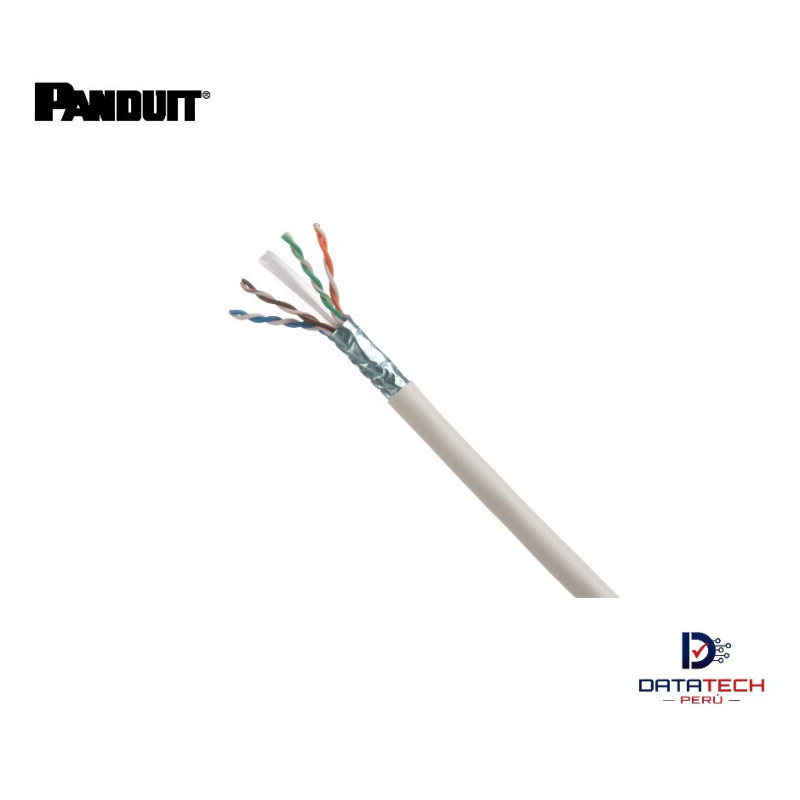
\includegraphics[width=4cm]{Componentes/01_cable_cat6a.jpg} \\
\end{tabular}
\end{table}

\begin{table}[H]
\centering
\renewcommand{\arraystretch}{1.3}
\begin{tabular}{p{9cm} p{4.5cm}}
\textbf{Patch Panel Modular 24P} \newline
\textit{Marca: CommScope --- Modelo: 760237040} \newline
Panel de conexión de 24 puertos, vacío/modular, para instalación en gabinetes MDF e IDF. &
\centering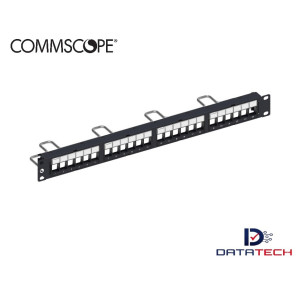
\includegraphics[width=4cm]{Componentes/02_patchpanel_24p.jpg} \\
\end{tabular}
\end{table}

\begin{table}[H]
\centering
\renewcommand{\arraystretch}{1.3}
\begin{tabular}{p{9cm} p{4.5cm}}
\textbf{Jack RJ45 Cat 6A Blindado MiniCom} \newline
\textit{Marca: Panduit --- Modelo: CJS6X88TGY} \newline
Módulo de conexión blindado, terminación por desplazamiento de aislante (IDC), contacto de 50 micras de oro. &
\centering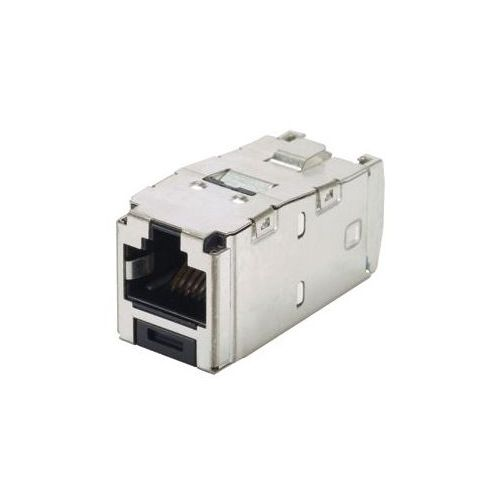
\includegraphics[width=4cm]{Componentes/03_jack_cat6a.jpg} \\
\end{tabular}
\end{table}

\begin{table}[H]
\centering
\renewcommand{\arraystretch}{1.3}
\begin{tabular}{p{9cm} p{4.5cm}}
\textbf{Patch Cord F/UTP Cat 6A 2.1m} \newline
\textit{Marca: Panduit --- Modelo: CO6X7BU} \newline
Cable de parcheo blindado, conectores RJ-45 moldeados con alivio de tensión. Uso: lado de usuario. &
\centering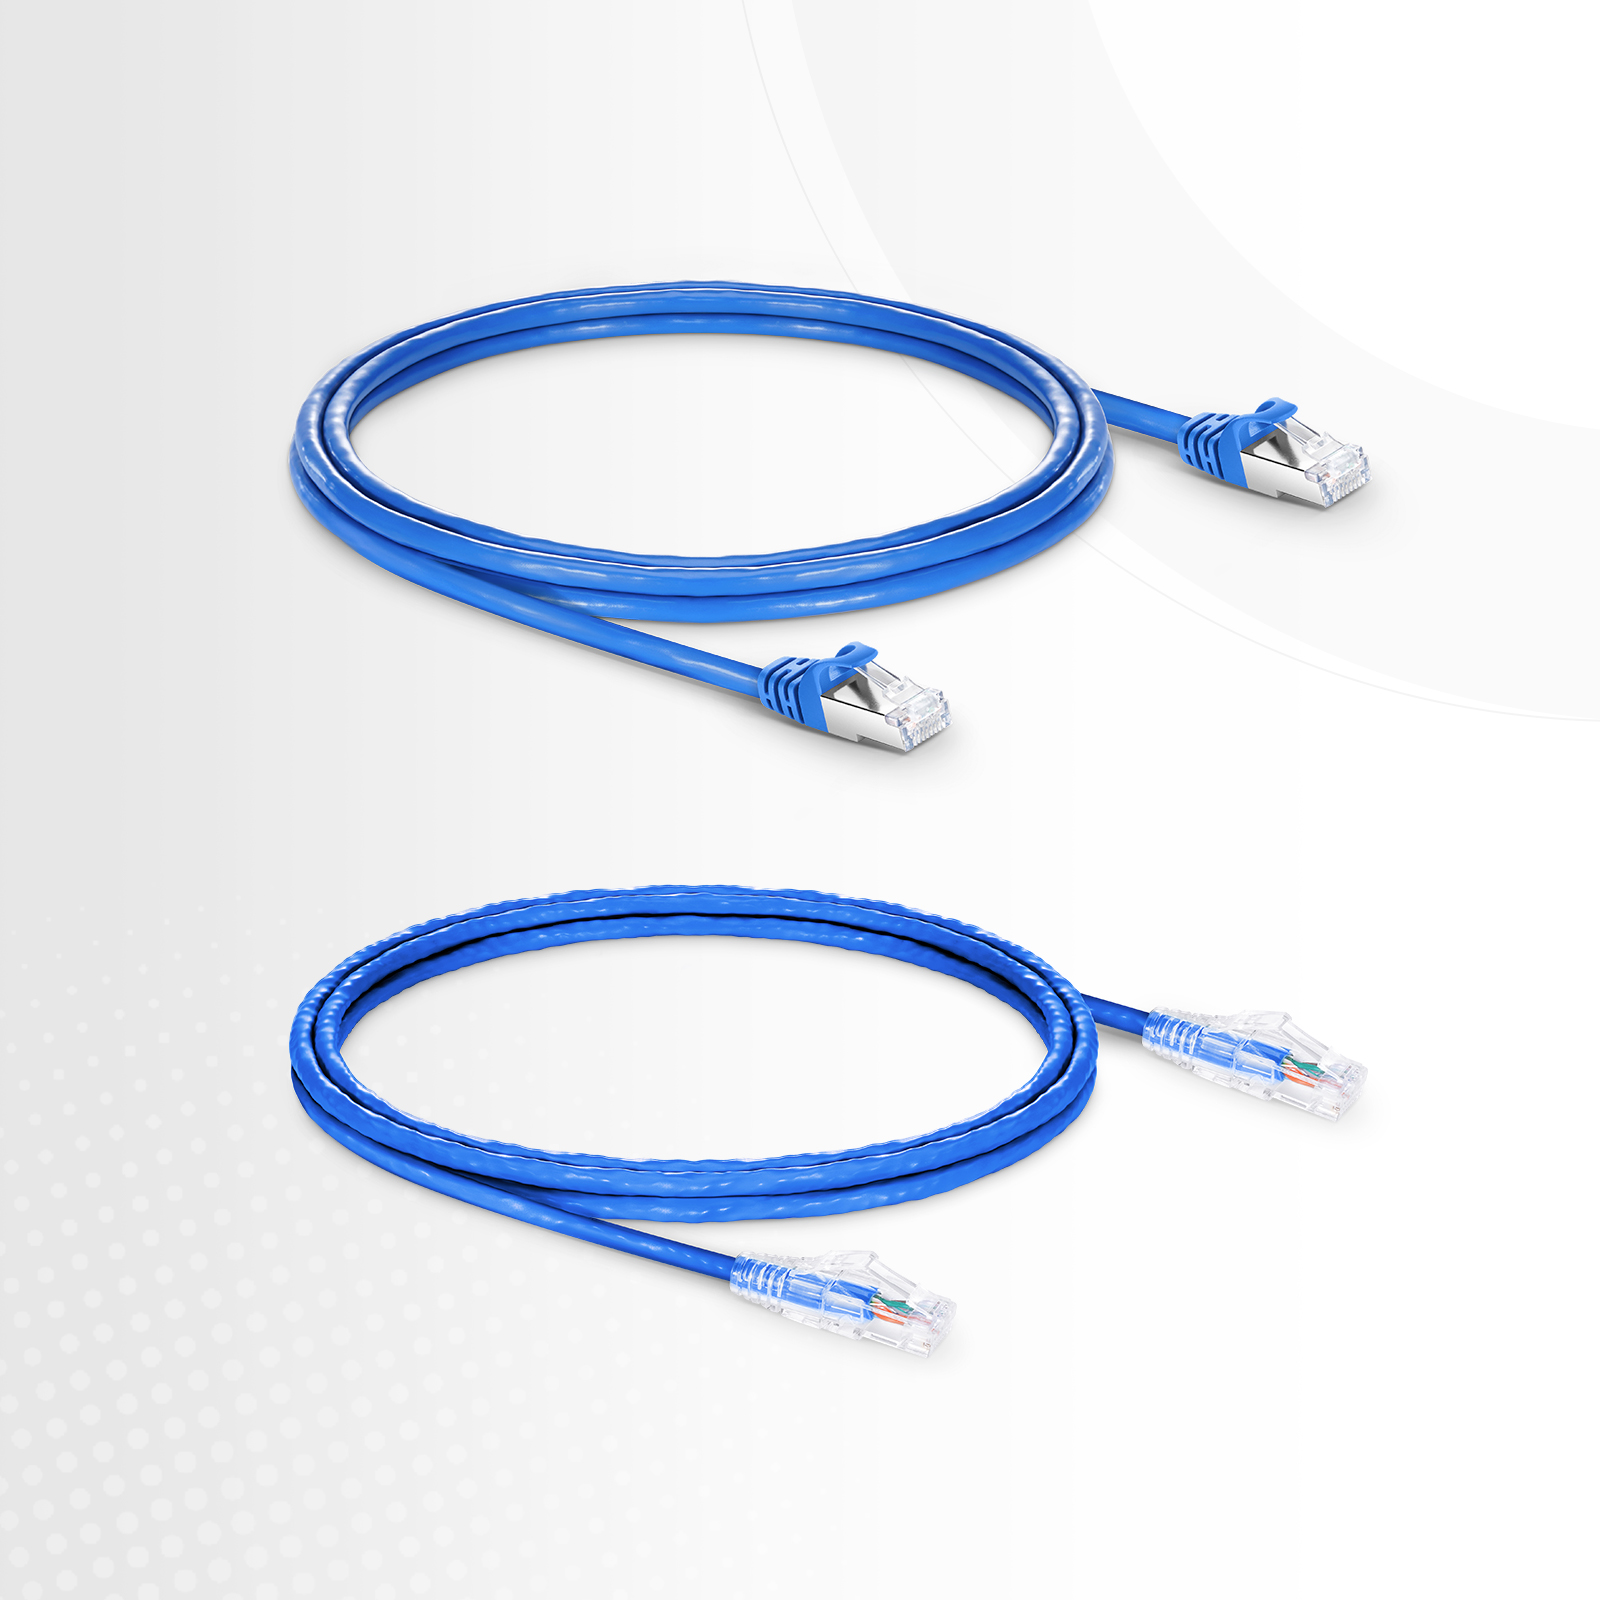
\includegraphics[width=4cm]{Componentes/04_patchcord_cat6a_2.1m.jpg} \\
\end{tabular}
\end{table}

\begin{table}[H]
\centering
\renewcommand{\arraystretch}{1.3}
\begin{tabular}{p{9cm} p{4.5cm}}
\textbf{Patch Cord F/UTP Cat 6A 1.0m} \newline
\textit{Marca: Panduit --- Modelo: CO6X3BU} \newline
Cable de parcheo blindado, conectores RJ-45 moldeados. Uso: lado de patch panel en gabinete. &
\centering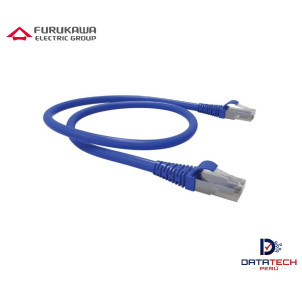
\includegraphics[width=4cm]{Componentes/05_patchcord_cat6a_1.0m.jpg} \\
\end{tabular}
\end{table}

\begin{table}[H]
\centering
\renewcommand{\arraystretch}{1.3}
\begin{tabular}{p{9cm} p{4.5cm}}
\textbf{Kit Fibra Óptica OM4} \newline
\textit{Marca: CommScope --- Serie: TeraSPEED} \newline
Fibra óptica multimodo de 4 hilos, chaqueta LSZH, optimizada para transmisión láser 10/40/100 Gbps. Backbone MDF--IDF. &
\centering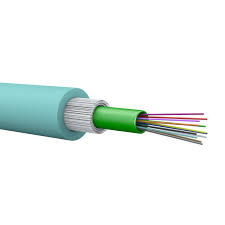
\includegraphics[width=4cm]{Componentes/06_kitfibraoptica_4hilos.jpg} \\
\end{tabular}
\end{table}

\begin{table}[H]
\centering
\renewcommand{\arraystretch}{1.3}
\begin{tabular}{p{9cm} p{4.5cm}}
\textbf{Faceplate 2 puertos} \newline
\textit{Marca: Panduit --- Modelo: CFPL2EIWH} \newline
Placa frontal color blanco con iconografía integrada para diferenciar datos, voz y CCTV. &
\centering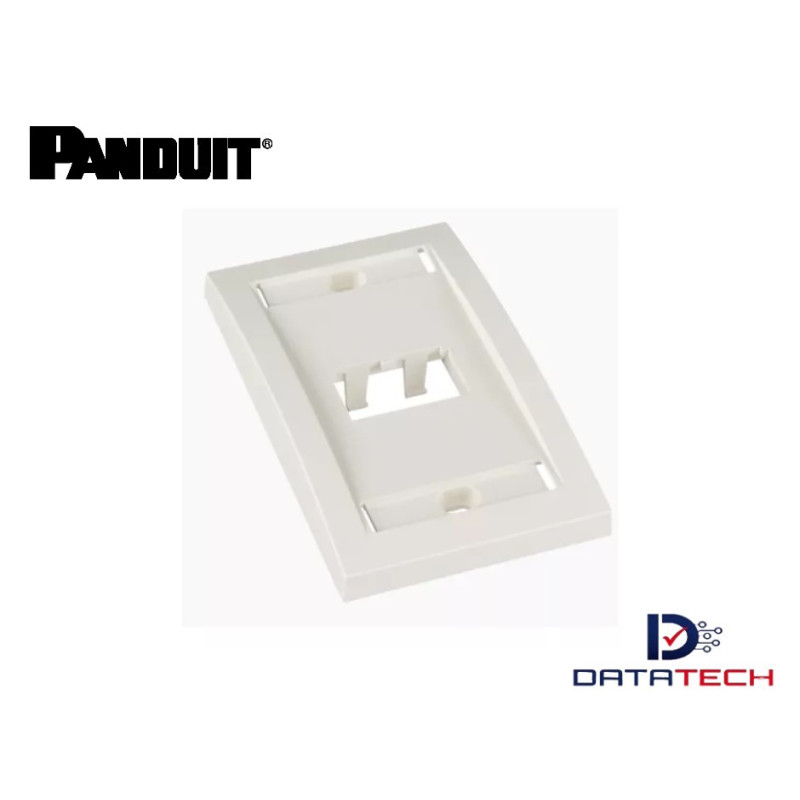
\includegraphics[width=4cm]{Componentes/07_faceplate_2puertos.jpg} \\
\end{tabular}
\end{table}

\begin{table}[H]
\centering
\renewcommand{\arraystretch}{1.3}
\begin{tabular}{p{9cm} p{4.5cm}}
\textbf{Caja Superficial PVC 1 Módulo} \newline
\textit{Marca: Panduit --- Modelo: CBX2EIWH} \newline
Caja de montaje superficial para faceplate, instalación sobre pared o canaleta. &
\centering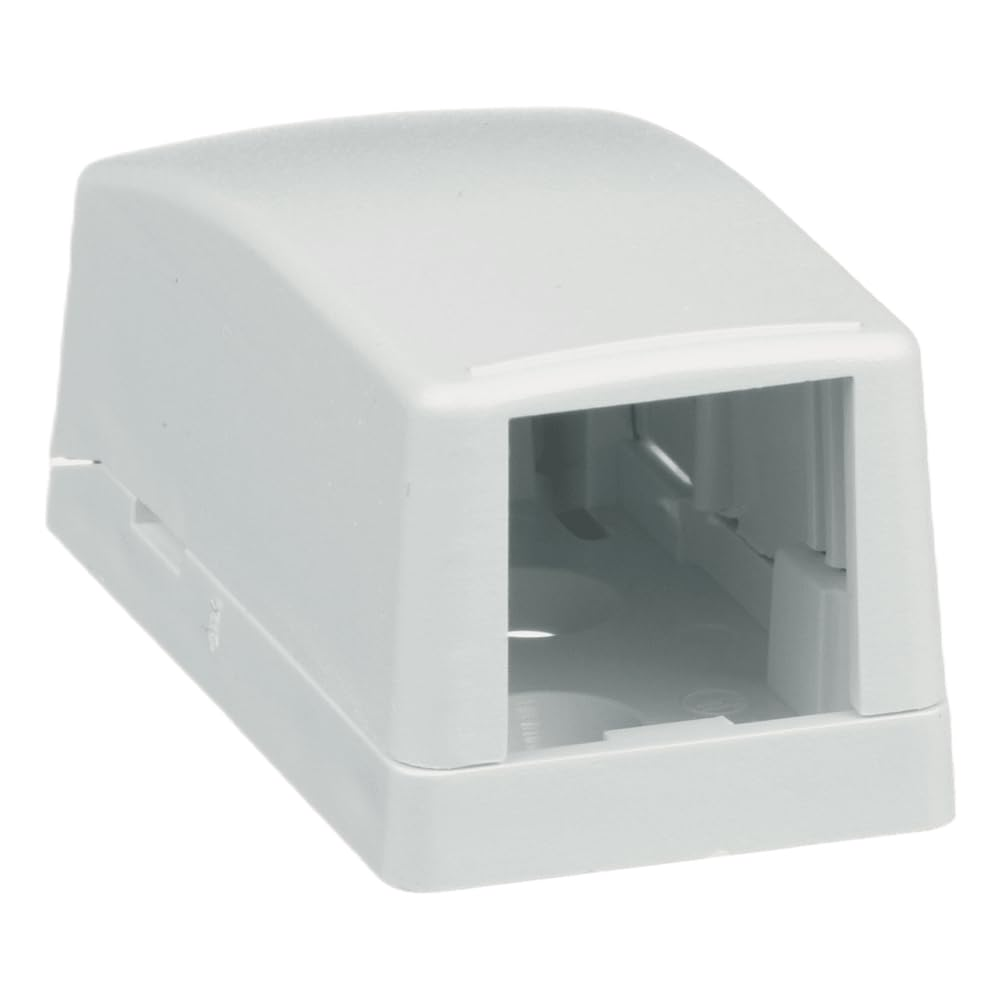
\includegraphics[width=4cm]{Componentes/08_cajasuperficial_1modulo.jpg} \\
\end{tabular}
\end{table}

\begin{table}[H]
\centering
\renewcommand{\arraystretch}{1.3}
\begin{tabular}{p{9cm} p{4.5cm}}
\textbf{Organizador Horizontal 1U} \newline
\textit{Marca: Tripp Lite --- Modelo: NR2600} \newline
Ducto ranurado frontal con tapa desmontable, instalado entre cada patch panel para guiado de cables. &
\centering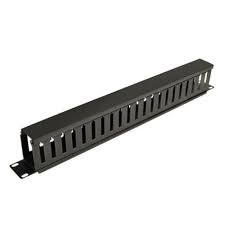
\includegraphics[width=4cm]{Componentes/09_organizadorhorizontal_1u.jpg} \\
\end{tabular}
\end{table}

\begin{table}[H]
\centering
\renewcommand{\arraystretch}{1.3}
\begin{tabular}{p{9cm} p{4.5cm}}
\textbf{Bandeja Porta-equipos 1U} \newline
\textit{Marca: Tripp Lite --- Modelo: RSD-1U} \newline
Bandeja estática para soporte de equipos no rackeables dentro del gabinete. &
\centering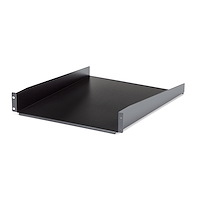
\includegraphics[width=4cm]{Componentes/10_bandejaportaequipos_1u.jpg} \\
\end{tabular}
\end{table}

\subsubsection*{Gabinetes de telecomunicaciones}

\begin{table}[H]
\centering
\renewcommand{\arraystretch}{1.3}
\begin{tabular}{p{9cm} p{4.5cm}}
\textbf{Gabinete de Piso 42U (MDF)} \newline
\textit{Marca: Tripp Lite --- Modelo: SR42UB} \newline
Gabinete cerrado de 19'' x 42U, puertas microperforadas, cerradura de seguridad. Ubicación: MDF-02, 2do piso. &
\centering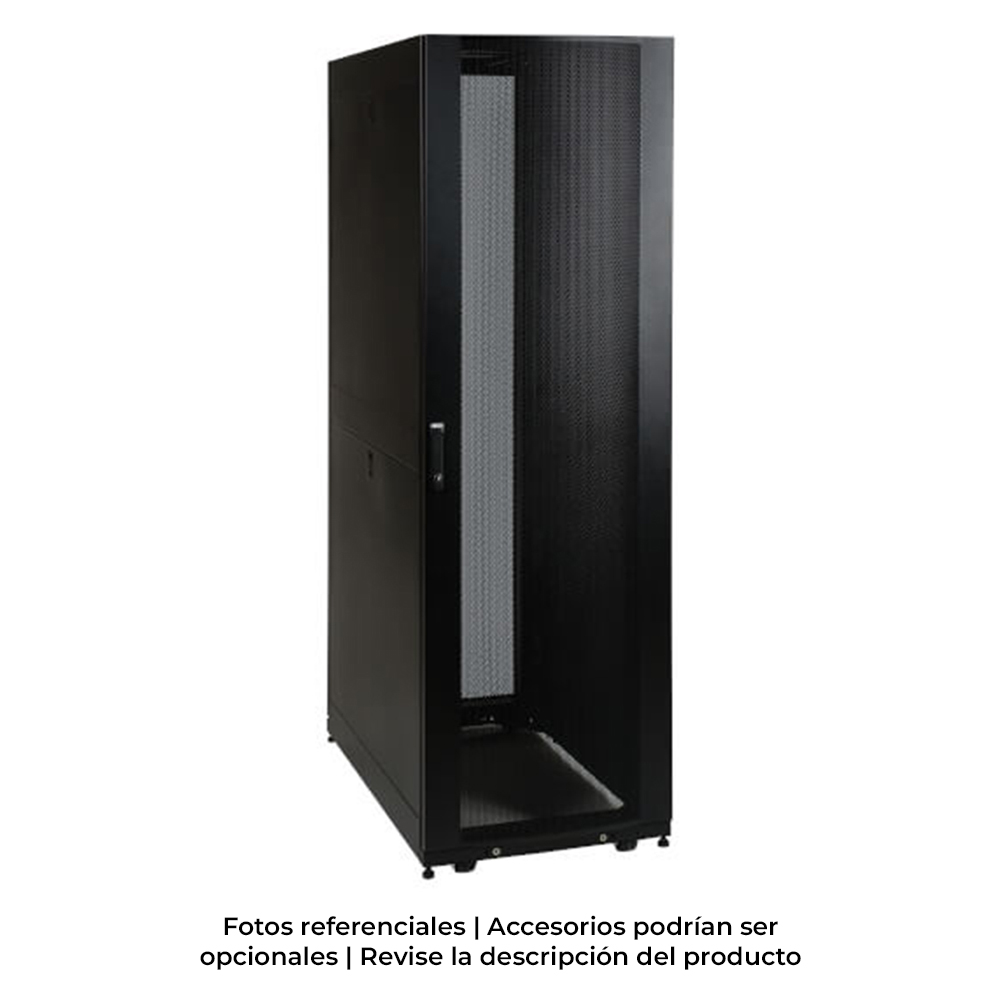
\includegraphics[width=4cm]{Componentes/11_gabinetepiso_42U.jpg} \\
\end{tabular}
\end{table}

\begin{table}[H]
\centering
\renewcommand{\arraystretch}{1.3}
\begin{tabular}{p{9cm} p{4.5cm}}
\textbf{Gabinete de Pared/Piso 24U (IDF)} \newline
\textit{Marca: Tripp Lite --- Modelo: SRW24US} \newline
Gabinete de 19'' x 24U. Se reutiliza este mismo modelo en los tres distribuidores de piso: IDF-01 (1er piso, nuevo), IDF-03 (3er piso) e IDF-04 (4to piso). &
\centering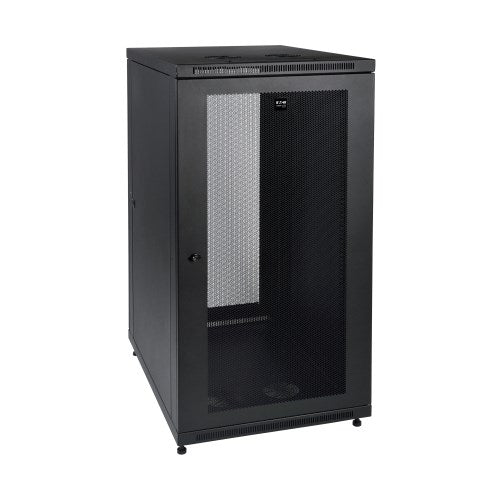
\includegraphics[width=4cm]{Componentes/12_gabinetepared_42U.jpg} \\
\end{tabular}
\end{table}

\subsubsection*{Puesta a tierra}

\begin{table}[H]
\centering
\renewcommand{\arraystretch}{1.3}
\begin{tabular}{p{9cm} p{4.5cm}}
\textbf{Barra de Tierra Principal (TMGB)} \newline
\textit{Marca: Panduit --- Modelo: TMGB-060} \newline
Barra de cobre perforada, punto de referencia de tierra para todo el sistema de telecomunicaciones. Ubicación: MDF, 2do piso. &
\centering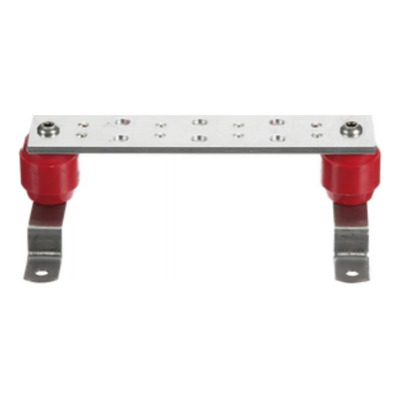
\includegraphics[width=4cm]{Componentes/13_barra_TMGB.jpg} \\
\end{tabular}
\end{table}

\begin{table}[H]
\centering
\renewcommand{\arraystretch}{1.3}
\begin{tabular}{p{9cm} p{4.5cm}}
\textbf{Barra de Tierra Secundaria (TGB)} \newline
\textit{Marca: Panduit --- Modelo: TGB-040} \newline
Barra secundaria instalada en cada IDF, interconectada a la TMGB. Se instalan 3 unidades (IDF-01, IDF-03, IDF-04). &
\centering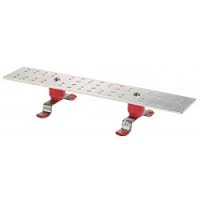
\includegraphics[width=4cm]{Componentes/14_barra_TGB.jpg} \\
\end{tabular}
\end{table}

\subsubsection*{Equipos activos}

\begin{table}[H]
\centering
\renewcommand{\arraystretch}{1.3}
\begin{tabular}{p{9cm} p{4.5cm}}
\textbf{Switch Catalyst 9200 48P PoE+} \newline
\textit{Marca: Cisco --- Modelo: C9200-48P-E} \newline
Switch de acceso Capa 2/3, 48 puertos PoE+, uplinks 10G SFP+ para backbone de fibra. &
\centering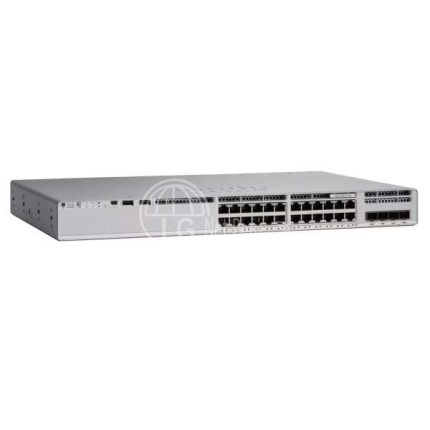
\includegraphics[width=4cm]{Componentes/15_switchcatalyst_ciscoc9200_24p.jpg} \\
\end{tabular}
\end{table}

\begin{table}[H]
\centering
\renewcommand{\arraystretch}{1.3}
\begin{tabular}{p{9cm} p{4.5cm}}
\textbf{Switch Catalyst 9200 24P PoE+} \newline
\textit{Marca: Cisco --- Modelo: C9200-24P-E} \newline
Switch de acceso 24 puertos PoE+, uplink 10G SFP+. Instalado en IDF-01 (1er piso, nuevo). &
\centering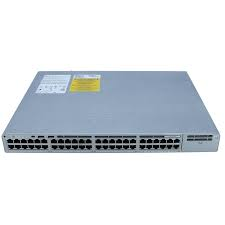
\includegraphics[width=4cm]{Componentes/16_switchcatalyst_ciscoc9200_48p.jpg} \\
\end{tabular}
\end{table}

\begin{table}[H]
\centering
\renewcommand{\arraystretch}{1.3}
\begin{tabular}{p{9cm} p{4.5cm}}
\textbf{Transceptor SFP+ 10G SR} \newline
\textit{Marca: Cisco --- Modelo: SFP-10G-SR} \newline
Módulo óptico multimodo para enlaces de backbone entre MDF y cada IDF. &
\centering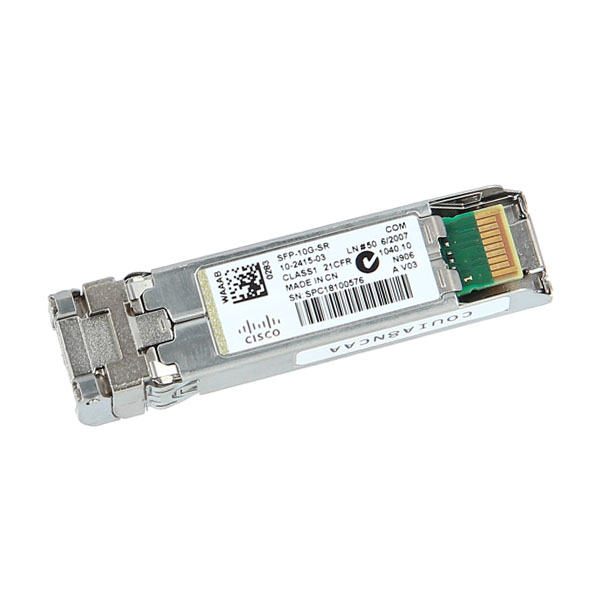
\includegraphics[width=4cm]{Componentes/17_transceptor_10gsr.jpg} \\
\end{tabular}
\end{table}

\begin{table}[H]
\centering
\renewcommand{\arraystretch}{1.3}
\begin{tabular}{p{9cm} p{4.5cm}}
\textbf{UPS Online 3kVA Rackeable} \newline
\textit{Marca: Tripp Lite --- Modelo: SU3000RTX} \newline
Sistema de alimentación ininterrumpida de doble conversión, autonomía mínima 15 min a plena carga. Uno por gabinete (4 unidades). &
\centering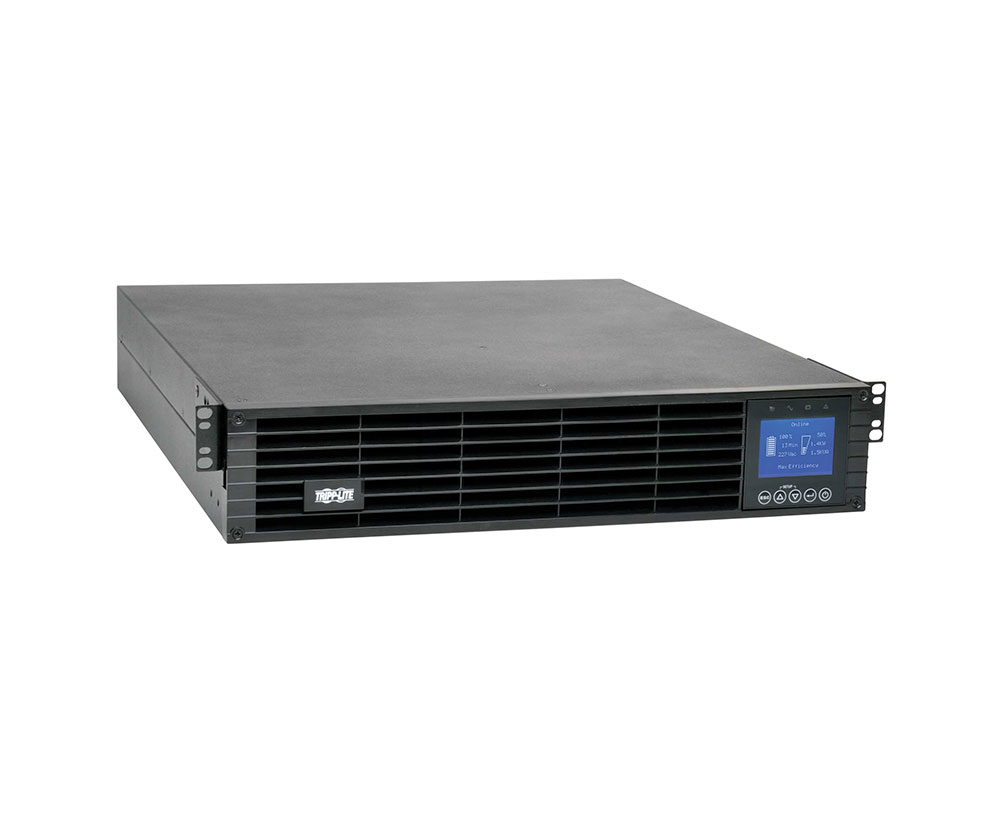
\includegraphics[width=4cm]{Componentes/18_upsonline_3kva.jpg} \\
\end{tabular}
\end{table}

\begin{table}[H]
\centering
\renewcommand{\arraystretch}{1.3}
\begin{tabular}{p{9cm} p{4.5cm}}
\textbf{Access Point WiFi 6 Interior} \newline
\textit{Marca: Cisco --- Modelo: C9120AXI} \newline
Punto de acceso doble banda, 802.11ax, alimentado por PoE+. &
\centering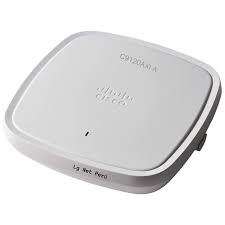
\includegraphics[width=4cm]{Componentes/19_accesspoint_wifi6.jpg} \\
\end{tabular}
\end{table}

\begin{table}[H]
\centering
\renewcommand{\arraystretch}{1.3}
\begin{tabular}{p{9cm} p{4.5cm}}
\textbf{Cámara IP Fija Interior 2MP} \newline
\textit{Marca: Dahua / Hikvision} \newline
Cámara IP con PoE+, resolución mínima 1920x1080, conectada a switches de acceso. &
\centering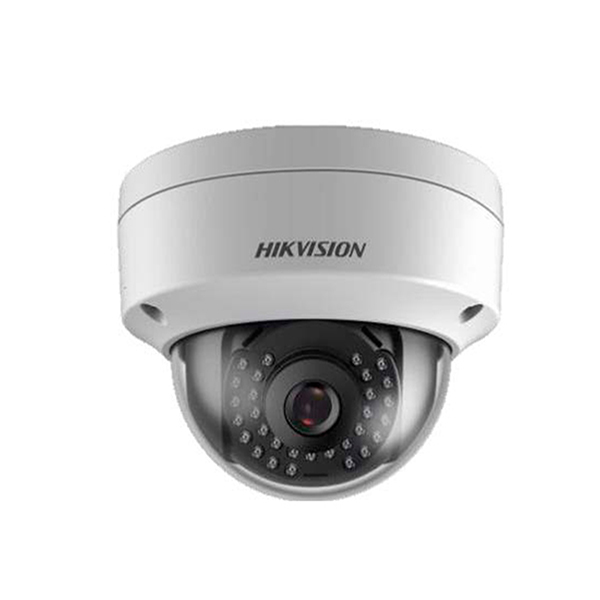
\includegraphics[width=4cm]{Componentes/20_camaraip_2mp.jpg} \\
\end{tabular}
\end{table}

\begin{table}[H]
\centering
\renewcommand{\arraystretch}{1.3}
\begin{tabular}{p{9cm} p{4.5cm}}
\textbf{NVR 16 Canales PoE+} \newline
\textit{Marca: Dahua / Hikvision} \newline
Grabador de video en red con HDD 4TB, ubicado en el gabinete MDF para gestión centralizada. &
\centering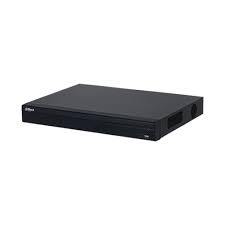
\includegraphics[width=4cm]{Componentes/21_nvr_16canales.jpg} \\
\end{tabular}
\end{table}

\subsubsection*{Canalizaciones}

\begin{table}[H]
\centering
\renewcommand{\arraystretch}{1.3}
\begin{tabular}{p{9cm} p{4.5cm}}
\textbf{Escalerilla Tipo Malla Electrozincada} \newline
\textit{Ancho: 300mm --- Norma: NEMA VE 1} \newline
Canalización principal (troncal) en pasillos, acero al carbono electrozincado. &
\centering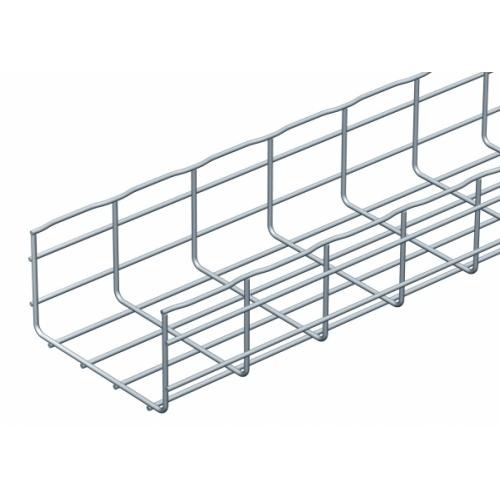
\includegraphics[width=4cm]{Componentes/22_escalerillaelectrozincada_300mm.jpg} \\
\end{tabular}
\end{table}

\begin{table}[H]
\centering
\renewcommand{\arraystretch}{1.3}
\begin{tabular}{p{9cm} p{4.5cm}}
\textbf{Canaleta PVC Doble Vía 40x20mm} \newline
\textit{Material: PVC rígido autoextinguible LSZH} \newline
Canalización secundaria con divisor físico para segregación datos/energía, adosada a pared. &
\centering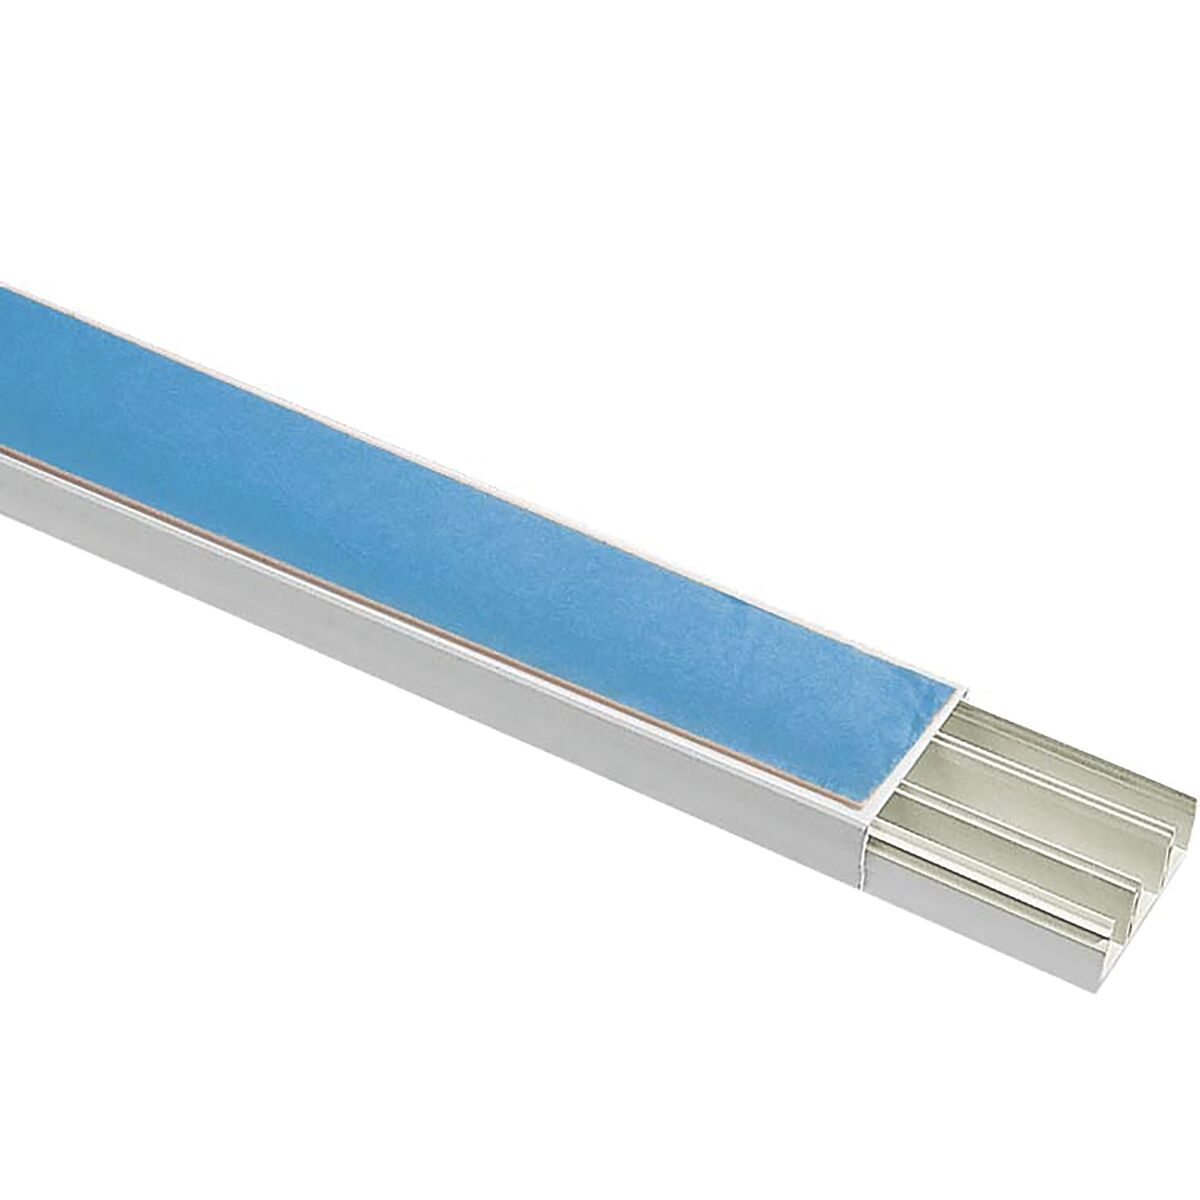
\includegraphics[width=4cm]{Componentes/23_canaletapvc_doblevia40x20mm_divisor.jpg} \\
\end{tabular}
\end{table}

\begin{table}[H]
\centering
\renewcommand{\arraystretch}{1.3}
\begin{tabular}{p{9cm} p{4.5cm}}
\textbf{Tubería Conduit EMT 1''} \newline
\textit{Material: Metálica} \newline
Protección del backbone de fibra óptica en pases verticales entre pisos. &
\centering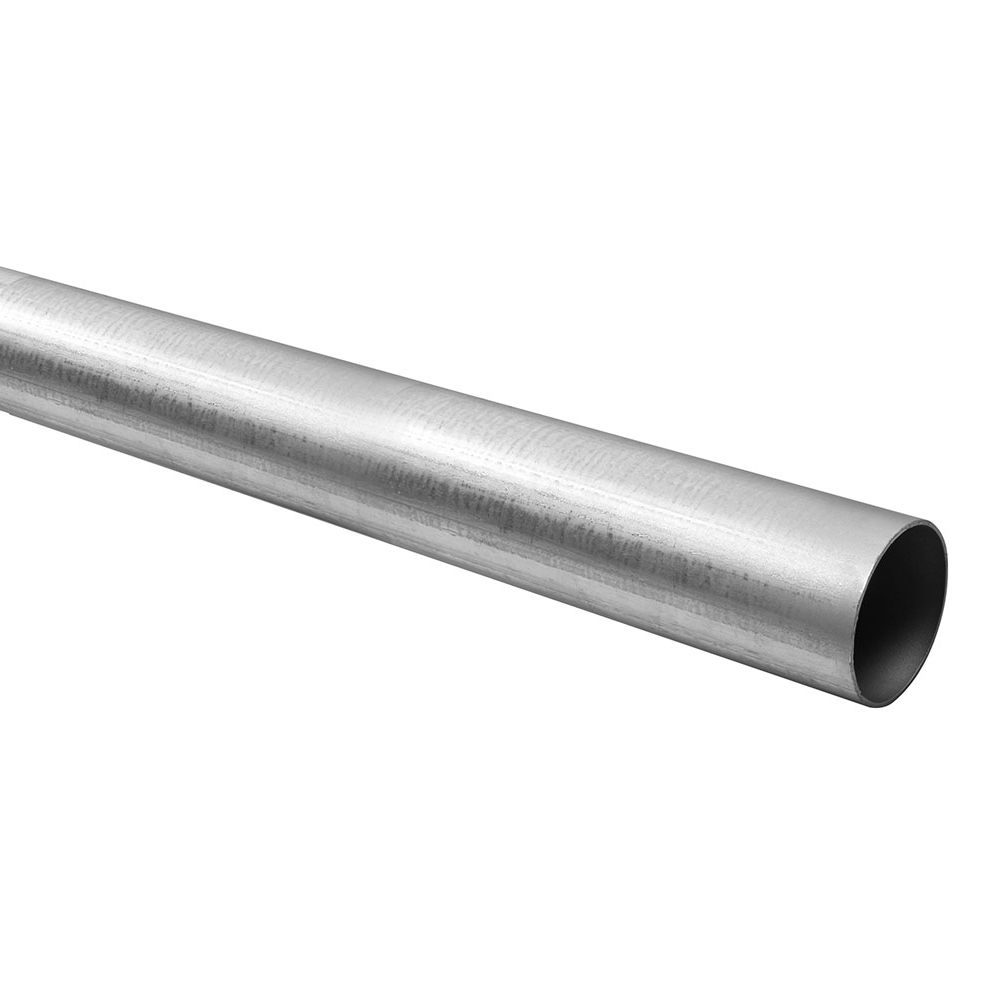
\includegraphics[width=4cm]{Componentes/24_tuberiaconduit_emt1''.jpg} \\
\end{tabular}
\end{table}

\begin{table}[H]
\centering
\renewcommand{\arraystretch}{1.3}
\begin{tabular}{p{9cm} p{4.5cm}}
\textbf{Caja de Registro Metálica} \newline
\textit{Uso: Paso y derivación de cableado} \newline
Instalada cada 15 m lineales de canalización y en cambios de dirección superiores a 30°. &
\centering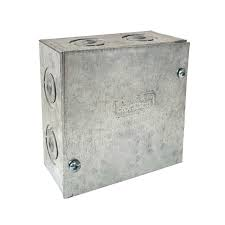
\includegraphics[width=4cm]{Componentes/25_cajaregistro_metalica.jpg} \\
\end{tabular}
\end{table}

\begin{table}[H]
\centering
\renewcommand{\arraystretch}{1.3}
\begin{tabular}{p{9cm} p{4.5cm}}
\textbf{Sello Cortafuego Intumescente} \newline
\textit{Uso: Pases de losa entre pisos} \newline
Mantiene la clasificación de resistencia al fuego de la estructura (mínimo RF-120). &
\centering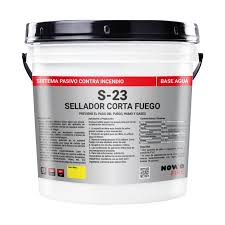
\includegraphics[width=4cm]{Componentes/26_selloconrtafuego_intumescente.jpg} \\
\end{tabular}
\end{table}

\subsubsection*{Certificación}

\begin{table}[H]
\centering
\renewcommand{\arraystretch}{1.3}
\begin{tabular}{p{9cm} p{4.5cm}}
\textbf{Certificador de Cableado Nivel IV} \newline
\textit{Marca: Fluke Networks --- Modelo: DSX-8000} \newline
Equipo de certificación de campo para validación de enlaces Cat 6A hasta 500 MHz. &
\centering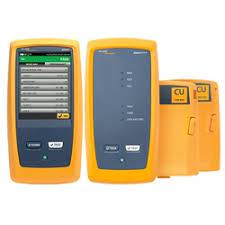
\includegraphics[width=4cm]{Componentes/27_certificadorfluke_dsx-8000.jpg} \\
\end{tabular}
\end{table}


\end{document}